% Options for packages loaded elsewhere
\PassOptionsToPackage{unicode}{hyperref}
\PassOptionsToPackage{hyphens}{url}
%
\documentclass[
]{article}
\usepackage{amsmath,amssymb}
\usepackage{lmodern}
\usepackage{iftex}
\ifPDFTeX
  \usepackage[T1]{fontenc}
  \usepackage[utf8]{inputenc}
  \usepackage{textcomp} % provide euro and other symbols
\else % if luatex or xetex
  \usepackage{unicode-math}
  \defaultfontfeatures{Scale=MatchLowercase}
  \defaultfontfeatures[\rmfamily]{Ligatures=TeX,Scale=1}
\fi
% Use upquote if available, for straight quotes in verbatim environments
\IfFileExists{upquote.sty}{\usepackage{upquote}}{}
\IfFileExists{microtype.sty}{% use microtype if available
  \usepackage[]{microtype}
  \UseMicrotypeSet[protrusion]{basicmath} % disable protrusion for tt fonts
}{}
\makeatletter
\@ifundefined{KOMAClassName}{% if non-KOMA class
  \IfFileExists{parskip.sty}{%
    \usepackage{parskip}
  }{% else
    \setlength{\parindent}{0pt}
    \setlength{\parskip}{6pt plus 2pt minus 1pt}}
}{% if KOMA class
  \KOMAoptions{parskip=half}}
\makeatother
\usepackage{xcolor}
\usepackage{graphicx}
\usepackage[margin=1in]{geometry}
\usepackage{wrapfig}
\usepackage{graphics}
\usepackage{titling}
\usepackage{fancyhdr}
\pagenumbering{gobble}
\addtocontents{toc}{\protect\thispagestyle{empty}}
\addtocontents{title}{\protect\thispagestyle{empty}}

\makeatletter
\def\maxwidth{\ifdim\Gin@nat@width>\linewidth\linewidth\else\Gin@nat@width\fi}
\def\maxheight{\ifdim\Gin@nat@height>\textheight\textheight\else\Gin@nat@height\fi}
\makeatother
% Scale images if necessary, so that they will not overflow the page
% margins by default, and it is still possible to overwrite the defaults
% using explicit options in \includegraphics[width, height, ...]{}
\setkeys{Gin}{width=\maxwidth,height=\maxheight,keepaspectratio}
% Set default figure placement to htbp
\makeatletter
\def\fps@figure{htbp}
\makeatother
\setlength{\emergencystretch}{3em} % prevent overfull lines
\providecommand{\tightlist}{%
  \setlength{\itemsep}{0pt}\setlength{\parskip}{0pt}}
\setcounter{secnumdepth}{-\maxdimen} % remove section numbering
\ifLuaTeX
  \usepackage{selnolig}  % disable illegal ligatures
\fi
\IfFileExists{bookmark.sty}{\usepackage{bookmark}}{\usepackage{hyperref}}
\IfFileExists{xurl.sty}{\usepackage{xurl}}{} % add URL line breaks if available
\urlstyle{same} % disable monospaced font for URLs
\hypersetup{
  pdftitle={Homework},
  pdfauthor={Joakim Bilyk},
  hidelinks,
  pdfcreator={LaTeX via pandoc}}

\title{Homework}
\usepackage{etoolbox}
\makeatletter
\providecommand{\subtitle}[1]{% add subtitle to \maketitle
  \apptocmd{\@title}{\par {\large #1 \par}}{}{}
}
\makeatother
\subtitle{Continuous time finance (FinKont)}
\author{Joakim Bilyk}
\date{January 26, 2023}

\begin{document}
%\maketitle

{
%title
\begin{titlepage}
\newcommand{\HRule}{\rule{\linewidth}{0.5mm}} % Defines a new command for the horizontal lines, change thickness here

\center % Center everything on the page
 
%----------------------------------------------------------------------------------------
%	HEADING SECTIONS
%----------------------------------------------------------------------------------------

\textsc{\LARGE University of Copenhagen}\\[4cm] % Name of your university/college
\textsc{\Large Continuous time finance
(FinKont)}\\[0.5cm] % Major heading such as course name
%\textsc{\large Assignment 1}\\[0.5cm] % Minor heading such as course title

%----------------------------------------------------------------------------------------
%	TITLE SECTION
%----------------------------------------------------------------------------------------

\HRule \\[0.4cm]
{ \huge \bfseries \thetitle}\\[0.4cm] % Title of your document
\HRule \\[1.5cm]
 
%----------------------------------------------------------------------------------------
%	AUTHOR SECTION
%----------------------------------------------------------------------------------------

\begin{minipage}{0.4\textwidth}
\begin{flushleft} \large
\emph{Author:}\\
\textsc{\theauthor} \\
\end{flushleft}
\end{minipage}
~
\begin{minipage}{0.4\textwidth}
\begin{flushright} \large
\emph{Date:} \\
\textsc{\thedate} \\
\end{flushright}
\end{minipage}\\[2cm]

% If you don't want a supervisor, uncomment the two lines below and remove the section above
%\Large \emph{Author:}\\
%John \textsc{Smith}\\[3cm] % Your name

%----------------------------------------------------------------------------------------
%	DATE SECTION
%----------------------------------------------------------------------------------------

%{\large \thedate}\\[2cm] % Date, change the \today to a set date if you want to be precise

%----------------------------------------------------------------------------------------
%	LOGO SECTION
%----------------------------------------------------------------------------------------


\includegraphics[height=200px, keepaspectratio]{logo_ku.png}\\[4cm] % Include a department/university logo - this will require the graphicx package
 
%----------------------------------------------------------------------------------------

\vfill % Fill the rest of the page with whitespace
\end{titlepage}
\setcounter{tocdepth}{5}
\tableofcontents
}
\thispagestyle{empty}
\newpage
\setcounter{page}{1}
\pagenumbering{arabic}
\pagestyle{fancy}
\hypertarget{introduction}{%
\section{Introduction}\label{introduction}}

\hypertarget{weeks}{%
\section{Weeks}\label{weeks}}

\hypertarget{week-1}{%
\subsection{Week 1}\label{week-1}}

\hypertarget{table-of-contents}{%
\subsubsection{Table of Contents}\label{table-of-contents}}

\begin{itemize}
\item
  \protect\hyperlink{the-brownian-motion}{Brownian motion (Chapter 4.1)}
\item
  \protect\hyperlink{conditional-expectation}{Conditional expectation
  (Appendix B.5)}
\item
  \protect\hyperlink{filtrations}{Filtration (Appendix B.3 and Chapter
  4.2)}
\item
  \protect\hyperlink{martingales}{Martingales (Appendix C.1 and Chapter
  4.4)}
\item
  \protect\hyperlink{discrete-time-models}{Introduction (Chapter 1)}
\item
  \protect\hyperlink{discrete-time-models}{Discrete time models (Chapter
  2 and 3)}
\item
  \protect\hyperlink{exercises-week-1}{Exercises}
\end{itemize}

\hypertarget{theory}{%
\subsubsection{Theory}\label{theory}}

This week revolves around the theory of the Brownian motion and
martingale processes. Other main topics are the binomial model and an
introduction to financial derivatives. Financial derivatives is
contingent on the outcome of a stochastic process at some future time
\(t=T\) and often is a function \(\Phi\) of some assets price \(S_t\).
As such the derivative will give a stochastic payout, at time \(t=T\) of
the size \(X_T=\Phi(S_T)\). Naturally we want to say something about the
\emph{fair} price of the derivative in the form of

\[\Pi_t(X_T)=\mathbb{E}\left[\Phi(S_T)\ \vert\ \mathcal{F}_t\right],\]

where \(\mathcal{F}_t\subset\mathcal{F}\) is the available information
at time \(t\). We will by defualt intepret the times \(t=0\) as
\emph{today} and \(t=T\) as \emph{tomorrow}. This indeed require some
fundamental understanding of the behaviour of the asset price \(S_t\).
This lead us over to discussing the process in center of the
\emph{Black-Scholes} model: the Brownian motion.

~

\hypertarget{the-brownian-motion}{%
\paragraph{The Brownian motion}\label{the-brownian-motion}}

\textbf{Definition 4.1.} \emph{(Brownian motion)} A stochastic process
\(W\) is called a \textbf{Brownian motion} or \textbf{Wiener process} if
the following conditions hold

\begin{enumerate}
\def\labelenumi{\arabic{enumi}.}
\tightlist
\item
  \(W_0=0\).
\item
  The process \(W\) has independent increments, i.e.~if \(r<s\le t< u\)
  then \(W_u-W_t\) and \(W_s-W_r\) are independent random variables.
\item
  For \(s<t\) the random variable \(W_t-W_s\) has the Gaussian
  distribution \(\mathcal{N}(0,t-s)\).
\item
  \(W\) has continuous trajectories i.e.~\(s\mapsto W(s;\omega)\) i
  continuous for all \(\omega \in\Omega\).
\end{enumerate}

\begin{wrapfigure}{R}{0.5\textwidth}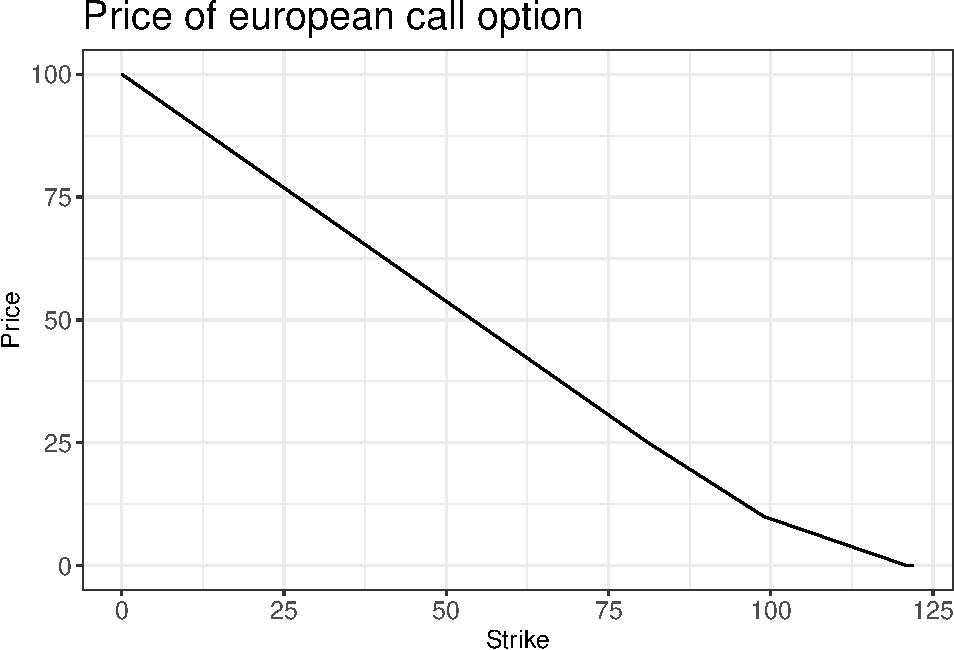
\includegraphics{/Users/joakimbilyk/Documents/GitHub/pdf/render/FinKont_homework_files/figure-latex/unnamed-chunk-4-1}\end{wrapfigure}

As one can see from the simulated sample path on the right, the Brownian
motion is rather irratic. In fact, the process varies infinitely on any
interval with length greater than 0. This gives some of the
characteristics of the process including that: \(W\) is continuous and
\(W\) is non-differential everywhere. This irratic behaviour is summed
up in the theorem.

\textbf{Theorem 4.2.} A Brownian motions trajectory \(t\mapsto W_t\) is
with probability one nowhere differential, and it has locally infinite
total variation.

This may seem not that horrifying since we can observe the process at
any time and conclude an increment \(W_{t+\Delta t}-W_t\) for any
\(\Delta t>0\) but any integral constructed with \(W_t\) as integrator
becomes nonsensible. We will be studying processes on the form

\[S_{t+\Delta t}-S_t=\mu(t,S_t)\Delta t+\sigma(t,S_t)\Delta W_t,\hspace{20pt}\Delta W_t=W_{t+\Delta t}-W_t.\]

where \(W_t\) is a standard Brownian motion and \(\mu(t,S_t)\) is
locally deterministic (velocity), that is \(\mu(t,S_t)\) is
deterministic on a small time interval. One could consider the dynamics
of the process \(S_t\) by studying the equation below as
\(\Delta t\to 0_+\)

\[\frac{S_{t+\Delta t}-S_t}{\Delta t}=\mu(t,S_t)+\sigma(t,S_t)\frac{W_{t+\Delta t}-W_t}{\Delta t}.\]

The limit however is impossible to determine as \(W_t\) is
non-differentiable and as such \(dS_t\) is not well-defined. From
LivStok we know that the dynamics of \(S_t\) is given by letting
\(\Delta t\) tend to 0 without dividing by it, that is

\[
dS_t=\mu(t,S_t)\ dt+\sigma(t,S_t)\ dW_t.
\]

Giving that \(S_0\) is observable we could intepret the dynamics on the
integral form

\[
S_t=S_0+\int_0^t\mu(s,S_s)\ ds+\int_0^t\sigma(s,S_s)\ dW_s,
\]

where the above integrals is Riemann-Stieltjes integral. This is however
still at dead-end, since from theorem 4.2 we know that \(W_t\) has
unbounded variation on any interval. So \textbf{we cannot define \(S_t\)
for each \(W\)-trajectory seperately} we will despite this define
another integral (the Ito integral) that in some other sense give a
global solution to this integral. To this we will be considering a
\(L^2\)-definition.

~

\hypertarget{conditional-expectation}{%
\paragraph{Conditional expectation}\label{conditional-expectation}}

The theory of conditional expectation is well-known from courses on the
bachelor. Because of this we will only summarise the most important
results.

We consider a background space \((\Omega,\mathcal{F},P)\) and a
sub-sigma algebra \(\mathcal{G}\subseteq \mathcal{F}\). We assume that
some stochastic variable is \(\mathcal{F}\)-measurable, that is the
mapping \(X : (\Omega,\mathcal{F},P) \to (\mathbb{R},\mathbb{B},m)\) is
\(\mathcal{F}-\mathbb{B}\)-measurable
i.e.~\(\forall B\in\mathbb{B} : \{X\in B\}\in\mathcal{F}\). For some
random variable \(Z\) defined on the subspace
\((\Omega,\mathcal{G},P)\), we say that \(Z\) is the conditional
expectation of \(X\) given \(\mathcal{G}\) if

\[
\forall G\in\mathcal{G} : \int_G Z(\omega)\ dP(\omega)=\int_G X(\omega)\ dP(\omega).
\]

This fact is summed up in the definition below.

\textbf{Definition B.27.} \emph{(Conditional expectation)} Let
\((\Omega,\mathcal{F},P)\) be a probability space and \(X\) a random
variable in \(L^1(\Omega,\mathcal{F},P)\) (\(\vert X\vert\) is
integrable). Let furthermore \(\mathcal{G}\) be a sigma-algebra such
that \(\mathcal{G}\subseteq \mathcal{F}\). If \(Z\) is a random variable
with the properties that:

\begin{enumerate}
\def\labelenumi{\roman{enumi}.}
\tightlist
\item
  \(Z\) is \(\mathcal{G}\)-measurable.
\item
  For every \(G\in\mathcal{G}\) it holds that
  \[\int_G Z(\omega)\ dP(\omega)=\int_G X(\omega)\ dP(\omega).\]
\end{enumerate}

Then we say that \(Z\) is the \emph{conditional expectation of \(X\)
given the sigma-algebra \(\mathcal{G}\)}. In that case we denote \(Z\)
by the symbol \(E[X\ \vert\ \mathcal{G}]\).

We see that from the above it always holds that \(X\) satisfies (ii). It
does not, however, always hold that \(X\) is \(\mathcal{G}\)-measurable.
Given this fact it is not trivial that a random variable
\(E[X\ \vert\ \mathcal{G}]\) even exists. This nontriviality is
fortunatly resolved by the Radon-Nikodym theorem.

\textbf{Theorem B.28.} \emph{(Existance and uniqueness of Conditional
expectation)} Let \((\Omega,\mathcal{F},P)\), \(X\) and \(\mathcal{G}\)
be given as in the definition above. Then the following holds:

\begin{itemize}
\tightlist
\item
  There will always exist a random variable \(Z\) satisfying conditions
  (i)-(ii) above.
\item
  The variable \(Z\) is unique, i.e.~if both \(Y\) and \(Z\) satisfy
  (i)-(ii) then \(Y=Z\) \(P\)-a.s.
\end{itemize}

This result ensures that we may condition on any sigma-algebra for
instance \(\mathcal{G}=\sigma(Y)\) in that case we (pure notation) write

\[
E[X\ \vert\ \sigma(Y)]=E[X\ \vert\ Y],\hspace{20pt}\sigma(Y)=\sigma\left(\left\{ Y\in A,\ A\in\mathbb{B}\right\}\right).
\]

In the above \(\sigma(Y)\) is simply the smallest sigma-algebra
containing all the pre-images of \(Y\), that is the smallest
sigma-algebra making \(Y\) measurable! Giving this foundation there are
a few properties conditional expectation have which is rather useful
(for instance the tower property).

Below we assume: Let \((\Omega,\mathcal{F},P)\) be a probability space
and \(X,Y\) be random variables in \(L^1(\Omega,\mathcal{F},P)\).

\textbf{Proposition B.29.} \emph{(Monotinicity/Linearity of Conditional
expectation)} The following holds:

\[X\le Y\ \Rightarrow\ E[X\ \vert\ \mathcal{G}]\le E[Y\ \vert\ \mathcal{G}],\hspace{20pt}P-\text{a.s.}\]
\[E[\alpha X + \beta Y\ \vert\ \mathcal{G}]=\alpha E[X\ \vert\ \mathcal{G}]+ \beta E[Y\ \vert\ \mathcal{G}],\hspace{20pt}\forall \alpha,\beta\in\mathbb{R}.\]

\textbf{Proposition B.30.} \emph{(Tower property)} Assume that it holds
that \(\mathcal{H}\subseteq\mathcal{G}\subseteq\mathcal{F}\). Then the
following hold:

\[E[E[X\vert \mathcal{G}]\vert\mathcal{H}]=E[X\vert \mathcal{H}],\]
\[E[X]=E[E[X\vert \mathcal{G}]].\]

\textbf{Proposition B.31.} Assume \(X\) is \(\mathcal{G}\) and that both
\(X,Y\) and \(XY\) are in \(L^1\) (only assuming \(Y\) is
\(\mathcal{F}\)-measurable), then

\[E[X\vert\mathcal{G}]=X,\hspace{20pt}P-\text{a.s.}\]
\[E[XY\vert\mathcal{G}]=XE[Y\vert\mathcal{G}],\hspace{20pt}P-\text{a.s.}\]

\textbf{Proposition B.32.} \emph{(Jensen inequality)} Let
\(f:\mathbb{R}\to\mathbb{R}\) be a convex (measurable) function and
assume \(f(X)\) is in \(L^1\). Then

\[f(E[X\vert\mathcal{G}])\le E[f(X)\vert\mathcal{G}],\hspace{20pt}P-\text{a.s.}\]

~

\hypertarget{filtrations}{%
\paragraph{Filtrations}\label{filtrations}}

Let \((\Omega,\mathcal{F},P)\) be a probability space. We define a
filtration as an increasing famility of sub-sigma-algebras in the
following definition.

\textbf{Definition B.16.} \emph{(Filtration)} Let
\(\mathbf{F}=(\mathcal{F}_t)_{t\ge 0}\) be an time indexed family of
sub-sigma-algebras such that \(F_s\subseteq F_t\) for \(s\le t\) and
\(\mathcal{F}_t\subseteq \mathcal{F}\) for all \(t\ge 0\). We may given
this filtration define \(\mathcal{F}_\infty\) as
\(\sigma\left(\bigcup_{t\ge 0}\mathcal{F}_t\right)\).

Filtrations is widely used in stochastic processes, as they allow for
the concept of knowledge/information. This is useful when considering
mean-values of future states but in an increasing information setting.
For this we introduce the term adapted processes.

\textbf{Definition B.17.} \emph{(Adapted process)} Let
\((\mathcal{F}_t)_{t\ge 0}\) be a filtration on the probability space
\((\mathcal{F}_t)_{t\ge 0}\). Furthermore, let \((X_t)_{t\ge 0}\) be a
stochastic process on the same space. We say that \(X_t\) is adapted to
the filtration \(\mathbf{F}\) if

\[X_t\ \text{ is }\ \mathcal{F}_t-\text{measurable},\hspace{20pt}\forall t\ge 0.\]

Obviously, we may introduce the \textbf{natural filtration}
\(\mathcal{F}^X_t\) given by the tragetory of the process \(X_t\):

\[\mathcal{F}^X_t=\sigma(\{X_s,\ s\le t\}).\]

Indeed, \(X_t\) is adapted to this filtration.

~

\hypertarget{martingales}{%
\paragraph{Martingales}\label{martingales}}

\textbf{Definition C.1.} Let \(M_t\) be a stochastic process defined on
a background space \((\Omega,\mathcal{F},P)\). Let
\((\mathcal{F}_t)_{t\ge 0}\) be a filtration. If \(M_t\) is adapted to
the filtration \(\mathcal{F}_t\), \(E\vert M_t\vert <\infty\) and

\[E[M_t\vert \mathcal{F}_s]=M_s,\hspace{20pt}P-\text{a.s.}\]

holds for any \(t>s\) we say that \(M_t\) is a martingale
(\(\mathbf{F}\)-martingale). If the above has \(\ge\) or \(\le\) we say
that \(M_t\) is either a \textbf{submartingale} or
\textbf{supermartingale} respectively.

Naturally, this defintions may easily be extended to discrete models and
we have the trivial equality:

\[E[M_t-M_s\ \vert\ \mathcal{F}_s]=0.\]

Martingales is useful, when proofing probalistic statements as the
posses tractable properties. A useful technique often include the
construction of the martingale

\[M_t=E[X\ \vert\ \mathcal{F}_t].\]

~

\hypertarget{discrete-time-models}{%
\paragraph{Discrete time models}\label{discrete-time-models}}

\hypertarget{one-period-time-models}{%
\paragraph{One-period time models}\label{one-period-time-models}}

The study of this course is the \textbf{European call} option (and
\emph{put} option). This financial derivative is an agreement between
two parties where the holder of the option has the right to
\emph{``exercise''} the derivative, at a future time \(t=T\). Exercising
means buying an asset at a certain agreed opon price-strike \(K\). In
the case of the put-option: the holder has the right (but not
obligation) to sell the asset at the strike price \(K\). As such the
derivative has the payoff

\[\text{Call}\ \text{option:}\hspace{10pt}\Phi(S_T)=(S_T-K)^+,\hspace{20pt}\text{Put}\ \text{option:}\hspace{10pt}\Phi(S_T)=(K-S_T)^+.\]

Our objective is to understand when an arbitrage exist and to find the
fair price of these derivative. The strategy in pricing is finding a
replicating portfolio with the same payoff as the option (with
probability one) and then price the derivative accordingly.

\hypertarget{model-description}{%
\subparagraph{Model description}\label{model-description}}

In the one-period model we consider the simplest possible market. We
have two distinct times \(t=0\) (today) and \(t=1\) (tomorrow) and we
may buy any portfolio as a mixture of bonds and one stock. We denote the
bonds price by \(B_t\) and the stocks price by \(S_t\) and we assume the
following:

\[
B_0=1,\ B_1=1+R,\hspace{20pt}S_0=s,\ S_1=\left\{\begin{matrix}s\cdot u, & with\ probability\ p_u.\\s\cdot d, & with\ probability\ p_d.\end{matrix}\right.
\]

We may introduce \(Z\) as the random variable

\[
Z=u\cdot (I)+d\cdot (1-I),
\]

for an bernoulli variable \(I\) with succes probability \(p_u\).
Naturally, we assume \(d\le (1+R)\le u\) (this is imperative to ensure
no arbitrage as we will see).

\hypertarget{portfolios-and-arbirtage}{%
\subparagraph{Portfolios and arbirtage}\label{portfolios-and-arbirtage}}

We study any portfolio on the \((B,S)\) market as a vector \(h=(x,y)\)
where \(x\) is the amount of bonds and \(y\) is the amount of stock held
in the portfolio. Notice that we allow for shorting, that is \(x<0\) or
\(y<0\). As such, we have that \(h\in \mathbb{R}^2\). In this we have
made some unrealistic, but attractable assumptions included in the
assumptions:

\begin{itemize}
\tightlist
\item
  We allow short positions and fractional holding,
  i.e.~\(h\in \mathbb{R}^2\),
\item
  We assume no spread between ask and bids,
\item
  No transaction costs and
\item
  A completely liquid market i.e.~we may borrow and buy as much stock
  and bonds as wanted.
\end{itemize}

Given that we have chosen a portfolio \(h\) we may introduce the value
process.

\textbf{Definition 2.1.} The \textbf{value process} of the porfolio
\(h\in\mathbb{R}^2\) is the stochastic process

\[V^h_t=xB_t+yS_t,\ t=0,1.\]

Given this notation we may define what an arbitrage is.

\textbf{Definition 2.2.} An \textbf{arbitrage} is a portfolio \(h\) with
the properties: 1) \(V^h_0=0\), 2) \(P(V^h_1\ge 0)=1\) and 3)
\(P(V^h_1>0)>0\).

That is \(h\) is an deterministic money-machine where we at least never
loose any money. Granted the bonds give a determinictic non-negative
return, but an arbitrage does not require any money out of pocket. With
the notion of an arbitrage we will show the first proposition regarding
the choice of \(R,u,d\) as defined above.

\textbf{Proposition 2.3.} The one-period binomial model is arbitrage
free if and only if the following inequality hold:

\[d\le (1+R)\le u.\tag{2.1}\]

\textbf{Proof.}

The statement is proofed by contradiction. Assume that \(d>1+R\) holds.
Then by definition \(u>d>1+R\). Notice that any portfolio satisfying
\(V_0^h=0\) must satisfy

\[0=xB_0+yS_0=x+ys\iff x=-ys\]

That is for some choice \(y\) the only arbitrage candidate is the
portfolio \(h=(-ys,y)\). Calculating the value at time \(t=1\) we have

\[V_1^h=-ys\cdot(1+R)+y\cdot s\cdot Z=ys(Z-1-R)\]

However since \(Z\ge d\) we have \(Z-(1+R)\ge 0\) and therefore an
arbitrage (for \(y>0\)). The other inequality \(1+R>u\) follows analog
steps. Simply choose some \(y<0\) and the result follows.
\(\blacksquare\)

From inequality (2.1) we see that since \(1+R\) is between \(u\) and
\(d\) we may find a pair \(q_d,q_u\ge 0\) with \(q_d+q_u=1\) such that

\[1+R=q_u\cdot u+q_d\cdot d.\]

This yields the important risk neutral valuation formula as summed op in
the following definition

\textbf{Definition 2.4.} A probability measure \(Q\) is called a
\textbf{martingale meausre} if the following condition holds:

\[S_0=\frac{1}{1+R}E^Q[S_1].\]

The above measure \(Q\) is the measure \(Q(Z=d)=q_d\) and \(Q(Z=u)=q_u\)
for the binomial model. This does in fact yield the risk neautral
valuation formula:

\begin{align*}
S_0&=\frac{1}{1+R}E^Q[S_1]=\frac{1}{1+R}(Q(Z=d)\cdot d\cdot s+Q(Z=u)\cdot u\cdot s)\\
&=s\frac{1}{1+R}(q_d\cdot d+q_u\cdot u)=s,
\end{align*}

where we simply use \(1+R=q_d\cdot d+q_u\cdot u\). We call this the risk
neautral valuation formula because it in some sense gives an expected
discounted value of the future stock price. We end this endavour with
reformulating the arbitrage proposition and determining the values of
the \(Q\)-measure.

\textbf{Proposition 2.5.} The one-period binomial model is arbitrage
free if and only if there exists a martingale measure \(Q\).

\textbf{Proposition 2.6.} The one-period binomial model has martingale
probabilities given by:

\[\left\{\begin{matrix}q_u=\frac{(1+R)-d}{u-d},\\ q_u=\frac{u-(1+R)}{u-d}.\end{matrix}\right.\]

\hypertarget{contingent-claims}{%
\subparagraph{Contingent Claims}\label{contingent-claims}}

This chapter revolves around the financial derivative and we start by
stating the definition of the financial derivative.

\textbf{Definition 2.7.} A \textbf{contingent claim} (financial
derivative) is \emph{any} stochastic variable \(X\) of the form
\(\Phi(Z)\), where \(Z\) is the stochastic varible driving the stock
price process.

We may also call the function \(\Phi\) the \textbf{contract function} as
it states how the contract is resolved once the stochastic variable
\(Z\) has been realised. Our objective is now to study, what a buyer of
said contract would have to pay at any given time \(t\). We call the
fair price of \(X\) at time \(t\): \(\Pi_t[X]\). As such it is easy to
see that the fair price at the time of maturity \(T\) is simply the
payout \(X\) i.e.~\(\Pi_T[X]=X\). Our strategy is to find a replicating
portfolio \(h\) and determine the price of said portfolio.

\textbf{Definition 2.8.} A contingent claim \(X\) can be
\textbf{replicated}, or said to be \textbf{reachable} if there exist a
portfolio \(h\) such that

\[
V_1^h=X,
\]

with probability one. In that case, we say that the portfolio \(h\) is a
\textbf{hedging} portfolio or a \textbf{replicationg} portfolio. If all
claims can be replicated we say that the market is \textbf{complete}.

Our pricing strategy is then to determine the value process of the
replicating portfolio and then by the first pricing principle below we
say that the price is imply the value of the replicating portfolio.

\textbf{Pricing principle 1.} If a clain \(X\) is reachable with
replicating portfolio \(h\), then the only reasonable price process for
\(X\) is given by

\[
\Pi_t[X]=V_t^h.
\]

Notice, that this assumes that a replicating portfolio exist and even so
we have a uniqueness statement to solve. We end this section by writing
two important results.

\textbf{Proposition 2.9.} Suppose that a claim \(X\) is reachable with
replicating portfolio \(h\). Then any price at time \(t\ge 0\) of the
claim \(X\) other than the value process of \(h\) will lead to an
arbitrage on the extended market \((B,S,X)\).

\textbf{Proposition 2.10.} If the one-period binomial model is free of
arbitrage, then it is also complete.

The hedging portfolio in the one-period binomial model is given by the
portfolio \((x,y)\) below

\[
x=\frac{1}{1+R}\cdot\frac{u\Phi(d)-d\Phi(u)}{u-d},\hspace{20pt}y=\frac{1}{s}\cdot\frac{\Phi(u)-\Phi(d)}{u-d}.
\]

\hypertarget{risk-neutral-valuation}{%
\subparagraph{Risk Neutral Valuation}\label{risk-neutral-valuation}}

We see that since the one-period model is complete we can price any
contingent claim and we see that

\begin{align*}
\Pi_0[X]&=\frac{1}{1+R}\cdot\frac{u\Phi(d)-d\Phi(u)}{u-d}+s\frac{1}{s}\cdot\frac{\Phi(u)-\Phi(d)}{u-d}\\
&=\frac{1}{1+R}\left\{\frac{u\Phi(d)-d\Phi(u)}{u-d}+(1+R)\frac{\Phi(u)-\Phi(d)}{u-d}\right\}\\
&=\frac{1}{1+R}\left\{\frac{(1+R)-d}{u-d}\Phi(u)+\frac{u-(1+R)}{u-d}\Phi(d)\right\}\\
&=\frac{1}{1+R}E^Q[X].
\end{align*}

i.e.~the price at time \(t=0\) should simply be the expected discounted
payout according to the martingale measure. This leads to the important
pricing proposition:

\textbf{Proposition 2.11.} If the one-period binomial model is free of
arbitrage, then the arbitrage free price of a contingent claim \(X\) is
given by

\[
\Pi_0[X]=\frac{1}{1+R}E^Q[X].\tag{2.4}
\]

Here the martingale measure \(Q\) is uniquely determined by the relation

\[
S_0=\frac{1}{1+R}E^Q[S_1],\tag{2.5}
\]

and the explicit expressions for \(q_u\) and \(q_d\) are given in
proposition 2.6. Furthermore the claim \(X\) can be replicated using the
portfolio

\begin{align*}
x&=\frac{1}{1+R}\cdot\frac{u\Phi(d)-d\Phi(u)}{u-d},\tag{2.6}\\
y&=\frac{1}{s}\cdot\frac{\Phi(u)-\Phi(d)}{u-d}.\tag{2.7}
\end{align*}

\hypertarget{multi-period-model}{%
\paragraph{Multi-period model}\label{multi-period-model}}

The one-period binomial model can easily be extended to a multi-period
model, by assuming that the bond and stock pricess evolve by the
processes:

\[
t\ge1:\ B_t=(1+R)B_{t-1}\hspace{20pt}\text{and}\hspace{20pt}B_0=1,
\]

\[
t\ge1:\ S_t=Z_{t-1}S_{t-1}\hspace{20pt}\text{and}\hspace{20pt}S_0=s,
\]

where we obviously have that \(B_t=(1+R)^t\) for \(t\ge 0\). In the
above \(Z_t\) is \(u\) with probability \(p_u\) and \(d\) with
probability \(p_d\). In this context, we need to define a portfolio in
terms of a strategy.

\textbf{Definition 2.13.} A \textbf{portfolio strategy} is a stochastic
process on \(\{1,...,T\}\)

\[
h=\left\{h_t=(x_t,y_t);\ t=1,...,T\right\}
\]

such that \(h_t\) is a function of \(S_0,S_1,...,S_{t-1}\). For a given
portfolio strategy \(h\) we set \(h_0=h_1\) by convention. The
associated \textbf{value process} corresponding to the portfolio \(h\)
is defined by

\[
V_t^h=x_t(1+R)+y_tS_t.
\]

Given this notation we may define what an arbitrage is, but first we
introduce the notion of a self-financing portfolio. A self-financing
portfolio in an intuative sense is a portfolio that is not withdrawn
from or deposited into.

\textbf{Definition 2.14.} A portfolio strategy \(h\) is said to be
\textbf{self-financing} if the following condition holds for all
\(t=0,...,T-1\):

\[
x_t(1+R)+y_tS_t=x_{t+1}+y_{t+1}S_t.
\]

The above equation says that the portfolio purchased at time \(t\) and
helt until \(t+1\) \((x_{t+1},y_{t+1})\) can only be financed by the
market value of the portfolio held from \([t-1,t)\)
i.e.~\((x_{t},y_{t})\). We now define an arbitrage.

\textbf{Definition 2.15.} An \textbf{arbitrage} is a self-financing
portfolio \(h\) with the properties: 1) \(V^h_0=0\), 2)
\(P(V^h_T\ge 0)=1\) and 3) \(P(V^h_T>0)>0\).

The multiperiod binomial model has an just like the oneperiod model a
result regarding when an arbitrage exists.

\textbf{Lemma 2.16.} If \(d\le (1+R)\le u\) then the multiperiod model
is arbitrage-free.

As one can see, the multiperiod model is rather similar to the one
period model. We wil in the following summarise equivalent statements
for the multiperiod model as the ones in the oneperiod model.

\textbf{Definition 2.17.} The martingale probabilities \(q_u\) and
\(q_d\) are defined as the probabilities for which the relation below
holds.

\[
s=\frac{1}{1+R}E^Q[S_{t+1}\ \vert\ S_t].
\]

\textbf{Proposition 2.18.} The martingale probabilities \(q_u\) and
\(q_d\) are given by

\[
\left\{\begin{matrix}q_u=\frac{(1+R)-d}{u-d},\\ q_u=\frac{u-(1+R)}{u-d}.\end{matrix}\right.
\]

\textbf{Definition 2.19.} A \textbf{contingent claim} is a stochastic
variable \(X\) of the form

\[
X=\Phi(S_T),
\]

where the \textbf{contract function} \(\mathbf{\Phi}\) is some given
real valued function.

\textbf{Definition 2.20.} A given contingent claim \(X\) is said to be
\textbf{reachable} if there exists a self-financing portfolio \(h\) such
that

\[
V_T^h=X,
\]

with probability one. In that case we say that the portfolio \(h\) is a
\textbf{hedging} portfolio or a \textbf{replicating} portfolio. If all
claims can be replicated we say that the market is \emph{(dynamically)}
\textbf{complete}.

\textbf{Pricing principle 2.} If a claim \(X\) is reachable with
replicating portfolio \(h\), then the only reasonable price process for
\(X\) os given by

\[
\Pi_t[X]=V_t^h,\ t=0,1,...,T.
\]

\textbf{Proposition 2.21.} Assume \(X\) is reachable by \(h\), then any
price other than \(V_t^h\) for some \(t\ge 0\) leads to an arbitrage
opportunity.

\textbf{Proposition 2.22.} The multiperiod model is complete, i.e.~every
claim can be replicated by a self-financing portfolio.

\textbf{Proposition 2.24.} \textbf{(Binomial algorithm)} Consider a
\(T\)-claim \(X=\Phi(S_T)\). Then this claim can be replicated using af
self-financing portfolio. If \(V_t(k)\) denotes the value of the
portfolio at the node \((t,k)\) (\(k\) referring to \(k\) amount of
up-moves for the stock), then \(V_t(k)\) can be computed recursively by
the scheme

\[
\left\{\begin{matrix}V_t(k)=\frac{1}{1+R}\left\{q_uV_{t+1}(k+1)+q_dV_{t+1}(k)\right\},\\ V_T(k)=\Phi(su^kd^{T-k}).\end{matrix}\right.
\]

where the martingale probabilities \(q_u\) and \(q_d\) are given by

\[
\left\{\begin{matrix}q_u=\frac{(1+R)-d}{u-d},\\ q_u=\frac{u-(1+R)}{u-d}.\end{matrix}\right.
\]

With the notation as above, the hedging portfolio is given by

\[
\left\{\begin{matrix}x_t(k)=\frac{1}{1+R}\cdot\frac{uV_t(k)-dV_t(k+1)}{u-d},\\ y_t(k)=\frac{1}{S_{t-1}}\cdot\frac{V_t(k+1)-V_t(k)}{u-d}.\end{matrix}\right.
\]

In particular, the arbitrage free price of the claim at \(t=0\) is given
by \(V_0(0)\).

\textbf{Example.}

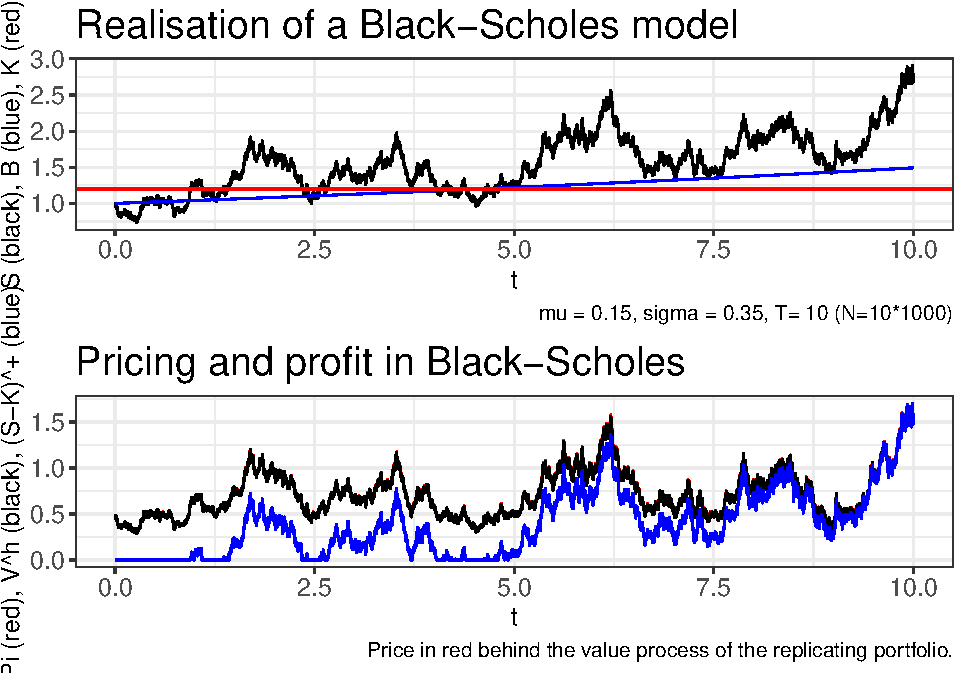
\includegraphics{/Users/joakimbilyk/Documents/GitHub/pdf/render/FinKont_homework_files/figure-latex/unnamed-chunk-5-1.pdf}

Consider \(R=0.04\), \(s=100\), \(u=1.1\), \(d=0.9\), \(p_u=0.6\) and
\(p_d=0.4\). We consider a model of length \(T=2\) and we want to
evaluate the price of the european call option with srike \(K=90\) that
is the contingent claim

\[
X=(S_T-K)^+,\hspace{20pt}\Phi(s)=(s-K)^+.
\]

For each time \(t\) we know the replicating portfolio, if we know the
payoff the following period. Therefore we start from the leaves of the
tree and work towards the root. Since the strike price is \(K=90\) the
end result will be the following payoffs:

\begin{align*}
u^2:\hspace{20pt}&(121-90)^+=31\\
ud:\hspace{20pt}&(99-90)^+=9\\
du:\hspace{20pt}&(99-90)^+=9\\
d^2:\hspace{20pt}&(81-90)^+=0
\end{align*}

Therefore by the risk neautral valuation formula with
\(q_u=\frac{(1+R)-d}{u-d}=0.7\) and \(q_d=\frac{u-(1+R)}{u-d}=0.3\) we
have that the cost of the replicating portfolio at time \(t=1\) is
respectively

\begin{align*}
u:\hspace{20pt}&\frac{1}{1+R}\left\{31\cdot q_u + 9 \cdot q_d\right\}\approx 23.46\\
d:\hspace{20pt}&\frac{1}{1+R}\left\{9\cdot q_u + 0 \cdot q_d\right\}\approx 6.06
\end{align*}

To replicate this payoff at time \(t=1\) we can use the risk neutral
valuation formula once more to find the base cost of the replicating
portfolio i.e.~the price of \(X\) at time \(t=0\)

\[
\frac{1}{1+R}\left\{23.46\cdot q_u + 6.06 \cdot q_d\right\}\approx 17.54.
\]

Working from the root to the leaves we can now calculate the hedging
portfolio at time \(t=0,1\) for each path. For time \(t=0\) we calculate

\begin{align*}
x=&\frac{1}{1+R}\cdot \frac{u\cdot 6.06-d\cdot 23.46}{u-d}\approx -69.46,\\
y=&\frac{1}{s}\cdot\frac{23.46-6.06}{u-d}\approx0.87
\end{align*}

We see by calculations that this does indeed replicate the payoff at
time \(t=1\):

\begin{align*}
u:\hspace{20pt}&V_1^h=(1+R)\cdot x + 110\cdot y\approx 23.46,\\
d:\hspace{20pt}&V_1^h=(1+R)\cdot x + 90\cdot y\approx 6.06.
\end{align*}

We also see by calculation that the initial portfolio does cost the
expected 17.54 as

\[
x\cdot 1+y\cdot100=87-69.46=17.54.
\]

Following these steps at time \(t=1\) the portfolios \((-86.54,1)\) (for
the up-scenario) and \((-38.94,0.5)\) (for the down-scenario) would
arise. Notice when calculating \(y\) one has to use the current price
\(S_1=S_0\cdot Z\) not \(S_0\). One should also check by similar
calculations as above, that these portfolios does indeed replicate the
payoff of the contingent claim \(X\). \(\square\)

\textbf{Proposition 2.25.} The arbitrage free price at \(t=0\) of a
\(T\)-claim \(X\) is given by

\[
\Pi_0[X]=\frac{1}{(1+R)^T}E^Q[X]
\]

where \(Q\) denotes the martingale measure, or more explicitly

\[
\Pi_0[X]=\frac{1}{(1+R)^T}\sum_{k=0}^T\binom{T}{k}q_u^kq_d^{T-k}\Phi(su^kd^{T-k}).
\]

\textbf{Example.}

\begin{wrapfigure}{R}{0.5\textwidth}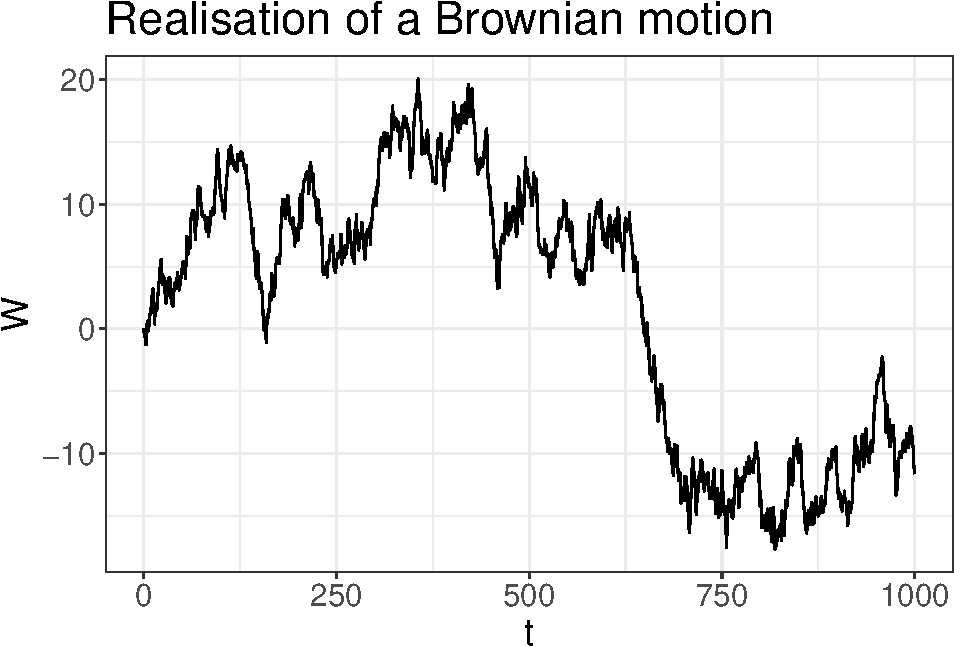
\includegraphics{/Users/joakimbilyk/Documents/GitHub/pdf/render/FinKont_homework_files/figure-latex/unnamed-chunk-7-1}\end{wrapfigure}

We follow an analog example as the one after proposition 2.24. Let
\(K=90\) and we see that

\begin{align*}
&\Pi_0[X]\\
&=\frac{1}{(1+0.04)^2}\sum_{k=0}^2\binom{2}{k}\cdot0.7^k\cdot0.3^{2-k}\cdot\Phi(100\cdot 1.1^k\cdot0.9^{2-k})\\
&=0.9245562\cdot\left(\underbrace{1\cdot 1\cdot0.09\cdot0}_{k=0}+\underbrace{2\cdot 0.7\cdot0.
3\cdot 9}_{k=1}+\underbrace{1\cdot 0.49\cdot1\cdot31}_{k=2}\right)\\
&=0.9245562\cdot\left(0+3.78+15.19\right)\\
&=17.53883
\end{align*}

Since we know that \(K\) must meaningfully range in \([0,121]\) we could
try to calculate the price of the contingent claim at time \(t=0\) for
all integers in this interval. We see that the price range between
\(S_0\) and 0 as expected. One can also see that the price changes slope
at the prices 99 and 121 as the function is linear in \(\Phi\) and som
realisations loose any effect on the price when the strike is higher
than the outcome. \(\square\)

\textbf{Proposition 2.26.} The condition \(d<(1+R)<u\) is necessary and
sufficient condition for absence of arbitrage.

\hypertarget{generelised-one-period-model}{%
\paragraph{Generelised one-period
model}\label{generelised-one-period-model}}

In the previous we had the simpel model where we only had one stochastic
asset \(S\) and only one stochastic variable \(Z\) determining the
future stock price. Now we will generelise this model by introducing
\(N\) assets and introducing som stochastic behaviour to the system.

\hypertarget{model-specification}{%
\subparagraph{Model specification}\label{model-specification}}

We consider the market consisting of a collection of stochastic prices
assets \(i=1,...,N\) with \(N\)-dimensional price process.

\[
S_t=\begin{bmatrix} S_t^1\\
\vdots\\
S_t^N\end{bmatrix}
\]

We now assume that \(S_t\) is defined on a background space with finite
sample space \(\Omega = \{\omega_1,...,\omega_M\}\) with associated
probabilities \(p_j=P(\omega_j)\), \(j=1,...,M\). We can then for eact
time \(t=1,...,T\) define the \(N\times M\) matrix \(D_t\) as such

\[
D_t=\begin{bmatrix} S_t^1(\omega_1)&\cdots &S_t^1(\omega_M)\\
\vdots &\ddots & \vdots\\
S_t^N(\omega_1) &\cdots&S_t^M(\omega_M)\end{bmatrix}.
\]

We will assume that \(S_0^1>0\) and \(S_1^1(\omega_j)>0\),
\(j=1,...,M\).

\hypertarget{absence-of-arbitrage}{%
\subparagraph{Absence of Arbitrage}\label{absence-of-arbitrage}}

We now define a \textbf{portfolio} as an \(N\)-dimensional row vector

\[
h=\begin{bmatrix} h^1, \dots,h^N\end{bmatrix}
\]

representing the amount of assets held at time \(t=0\) and held until
\(t=1\). The \textbf{value process} is then

\[
V^h_t=h\cdot S_t=\sum_{i=1}^N h^iS_t^i,\ t=0,1.
\]

For a given \(\omega_j\in\Omega\) we have the realisation

\[
V_t^h=hS_t(\omega_j)=hd_j=(hD)_j.
\]

\textbf{Definition 3.1.} The portfolio \(h\) is an \textbf{arbitrage
portfolio} fil it satisfies the conditions: \(V_0^h=0\),
\(P(V_1^h\ge 0)=1\) and \(P(V_1^h>0)>0\).

\textbf{Lemma 3.2.} \textbf{(Farkas' Lemma)} Suppose that
\(d_0,d_1,...,d_M\) are column vectors in \(\mathbb{R}^N\). Then exactly
one of the following problems possesses a solution.

\begin{itemize}
\tightlist
\item
  \textbf{Problem 1}: There exist \(\lambda_1,...,\lambda_M\ge0\) such
  that \(d_0=\sum_{j=1}^M\lambda_jd_j\).
\item
  \textbf{Problem 2}: There exist \(h\in\mathbb{R}^N\) such that
  \(h^\top d_0<0\) and \(h^\top d_j\ge 0\) for \(j=1,...,M\).
\end{itemize}

We now investegate this system for any possible arbitrage portfolios.
However first we acknowledge that there exist a nominal price system
\(S_t\) and a normalised price system \(Z_t\). The latter we define as
the nominel pricess under the numeraire \(S_t^1\) that is

\[
Z_t=\begin{bmatrix} S_t^1/S_t^1\\
S_t^2/S_t^1\\
\vdots\\
S_t^N/S_t^1\end{bmatrix}=\begin{bmatrix} 1\\
S_t^2/S_t^1\\
\vdots\\
S_t^N/S_t^1\end{bmatrix}.
\]

The reason for introducing the normalized price system is that we can
without much effort translate results in this system to the nominal
system and the normalised system is easier to analize. For this,
however, we need af few results.

\textbf{Lemma 3.3.} With notation as above, the following hold.

\begin{enumerate}
\def\labelenumi{\arabic{enumi}.}
\tightlist
\item
  The \(Z_t\) value process i related to the \(S_t\) value process by \[
    V_t^{h,Z}=hZ_t=\frac{1}{S_t^1}V_t^h.
    \]
\item
  A portfolio is an arbitrage in the \(S_t\) system if and only if there
  is an arbitrage in the \(Z_t\) system.
\item
  In the \(Z_t\) price system, the numeraie asset \(Z^1\) has unit
  constant prices i.e.~\(Z_t^1=1\) for all \(t\ge 0\).
\end{enumerate}

One of the reason that the normalised system is attractable is that the
numeraire asset is constant i.e.~risk free in the normalised system. Let
us formulate our first main result.

\textbf{Proposition 3.4.} The market is arbitrage free if and only iff
there exists strictly positive real numbers \(q_1,...,q_M\ge 0\) with
\(q_1+\cdots + q_M=1\) (probability vector) such that the following
vector equality holds

\[
\begin{bmatrix} Z_0^1\\
\vdots\\
Z_N^1\end{bmatrix}=\begin{bmatrix} Z_1^1(\omega_1)\\
\vdots\\
Z_1^N(\omega_1)\end{bmatrix}q_1+\cdots +\begin{bmatrix} Z_1^1(\omega_M)\\
\vdots\\
Z_1^N(\omega_M)\end{bmatrix}q_M.\tag{3.3}
\]

\textbf{Proof.}

\hypertarget{martingale-measures}{%
\subparagraph{Martingale Measures}\label{martingale-measures}}

\textbf{Definition 3.5.} Given the objective probability measure \(P\)
on \((\Omega,\mathcal{F},P)\), we say that another probability measure
\(Q\) defined on \(\Omega\) is \textbf{equivalent} to \(P\) if

\[
\forall A\in\mathcal{F}:P(A)=0\iff Q(A)=0,
\]

or equivalently

\[
\forall A\in\mathcal{F}:P(A)=1\iff Q(A)=1.
\]

\textbf{Definition 3.7.} Consider the market model above and set \(S^1\)
as the numeraire asset. We say that a probability measure \(Q\) defined
on \(\Omega\) is a \textbf{martingale measure} if it satisfies the
following conditions:

\begin{enumerate}
\def\labelenumi{\arabic{enumi}.}
\tightlist
\item
  \(Q\) is equivalent to \(P\), i.e.~\(Q\sim P\).
\item
  For every \(i=1,...,N\), the normalized asset price process \[
    Z_t^i=\frac{S_t^i}{S_t^1},
    \] is martingale under the measure \(Q\).
\end{enumerate}

\textbf{Theorem 3.8.} \textbf{(First Fundamental Theorem)} Given a fixed
numeraire, ther market is free of arbitrage possibilities if and only if
there exists a martingale measure \(Q\).

By assuming that the numeraire asset is risk free (i.e.~does not depend
on \(\omega\)) then by scaling we can derive the short interest rate as

\[
1+R=\frac{S_1^1}{S_0^1}.
\]

With this in mind we can formulate theorem 3.8 in its more widely used
form.

\textbf{Theorem 3.9.} \textbf{(First Fundamental Theorem)} Assume that
there exist a risk free asset, and denote the corresponding risk free
interest rate by \(R\). Then the market is arbitrage free if and only if
there exist a measure \(Q\sim P\) such that

\[
S_0^i=\frac{1}{1+R}E^Q[S_1^i],\hspace{20pt}\text{for all}\ i=1,...,N.\tag{3.9}
\]

\hypertarget{martingale-pricing}{%
\subparagraph{Martingale Pricing}\label{martingale-pricing}}

Moving forward we will assume that there exist a risk free asset and we
will denote it by \(B_t\) (\(B_t=S^1_t/S^1_0\)).

\textbf{Definition 3.10.} A \textbf{contingent claim} is any random
variable \(X\), defined on the sample space \(\Omega\).

To ensure no arbitrage in the extended market containing the \(N\)
assets and the contingent claim we can apply the first fundamental
pricing theorem on the extended market.

\textbf{Proposition 3.11.} Consider a given claim \(X\). In order to
avoid arbitrage, \(X\) must then be priced according to the formula

\[
\Pi_0[X]=\frac{1}{1+R}E^Q[X],\tag{3.10}
\]

where \(Q\) is a martingale measure for the underlying market
\((\Pi,S^1,...,S^N)\).

\hypertarget{completeness}{%
\subparagraph{Completeness}\label{completeness}}

Given that a market is arbitrage-free we may run into a uniqueness issue
when determining the price of a contingent claim. If a martingale
measure exist we will very much like it to be unique as this will ensure
that the price from the risk neutral valuation formula is unique. To
this we need the market to be complete.

\textbf{Definition 3.12.} Consider a contingent claim \(X\). If there
exists a portfolio \(h\), based on the underlying assets, such that

\[
V_1^h=X,\ \text{with probability 1}\tag{3.11}
\]

i.e.

\[
V_1^h(\omega_j)=X(\omega_j),\ j=1,...,M,\tag{3.12}
\]

then we say that \(X\) is \textbf{replicated}, or \textbf{hedged} by
\(h\). Such a portfolio \(h\) is called a replicating, or hedging
portfolio. If every contingent claim can be replicated, we say that the
market is \textbf{complete}.

We can now formulate a proposition on when the market is complete in
terms of the matrix \(D\).

\textbf{Proposition 3.13.} The market is complete if and only if the
rows of the matrix \(D\) span \(\mathbb{R}^M\), i.e.~if and only if
\(D\) has rank \(M\).

Now we formulate the second fundamental pricing theorem in terms of the
martingale measure \(Q\).

\textbf{Proposition 3.14.} \textbf{(Second Fundamental Theorem)} Assume
that the model is arbitrage free i.e.~\(Q\) exist. Then the market is
unique if and only if the martingale measure is unique.

\hypertarget{stochastic-discount-factors}{%
\subparagraph{Stochastic Discount
Factors}\label{stochastic-discount-factors}}

\textbf{Definition 3.16.} The random variable \(L\) on \(\Omega\) is
defined by

\[
L(\omega_i)=\frac{q_i}{p_i},\hspace{20pt} i=1,...,M.
\]

\textbf{Definition 3.17.} Assume the absence of arbitrage, and fix a
martingale measure \(Q\). With notation as above, the \textbf{stochastic
discount factor} (or ``state price deflator'') is the random variable
\(\Lambda\) on \(\Omega\) by

\[
\mathbf{M}(\omega)=\frac{1}{1+R}\cdot L(\omega).\tag{3.19}
\]

\textbf{Proposition 3.18.} The arbitrage free price of any claim \(X\)
is given by the formula

\[
\Pi_0[X]=E^P[\mathbf{M}\cdot X]
\]

where \(\mathbf{M}\) is a stochastic discount factor.

~

\hypertarget{exercises-week-1}{%
\subsubsection{Exercises Week 1}\label{exercises-week-1}}

\textbf{Probability exercises}

Let \((W(t))_{t\ge}\) be a Brownian motion (Bjork, Definition 4.1).

\textbf{Exercise 1.} Show that the following processes also are Brownian
motions.

\begin{enumerate}
\def\labelenumi{\roman{enumi}.}
\tightlist
\item
  \((-W(t))_{t\ge 0}\) (symmetry)
\item
  For any \(s\ge 0\), \((W(t+s)-W(s))_{t\ge 0}\) (time-homogeneity).
\item
  For every \(c>0\), \((cW(t/c^2))_{t\ge 0}\) (scaling).
\end{enumerate}

\textbf{Solution (i).}

By assumption \(W\) is a Brownian motion and so it follows that

\[-W_0=-1\cdot0=0\]

Furthermore, for \(r<s\le t< u\) it holds that \(W_u-W_t\) and
\(W_s-W_r\) is independent. By seperate transformations the independence
property is preserved and \(-(W_u-W_t)\) and \(-(W_s-W_r)\) is
independent. Next, for a normal distributed random variable
\(N\sim\mathcal{N}(\mu,\sigma^2)\) it holds, that for a scaler
\(c\in\mathbb{R}\) we have \(c N\sim\mathcal{N}(c\mu,c^2\sigma ^2)\).
Then obviously;

\[-(W_t)=(-1)W_t\stackrel{d}{=}\mathcal{N}((-1)\cdot0,(-1)^2(t-s))\stackrel{d}{=}\mathcal{N}( 0,t-s).\]

Lastly, let \(\omega \in \Omega\) and consider the sample path
\(s\mapsto (-W_s)(\omega)\). Clearly for two continuous functions \(f\)
and \(g\) it holds that \((g\circ f)\) is continuous. Then with
\(g(f)=-f\) and \(f(t)=W_t(\omega)"/>\) it follows that
\((-W_t)=(g\circ W)(t)\) is also continuous.

\textbf{Solution (ii).}

Much like the previous exercise we define a new process and show the
properties hold. Let \(s\ge 0\) be chosen arbitrary. Now define
\(X_t=W(t+s)-W(s)\).

First, we let \(t=0\) and see

\[X_0=W(0+s)-W(s)=W(s)-W(s)=0.\]

Secondly, we have that for \(r<u\):

\[X_u-X_r=W(u+s)-W(s)-(W(r+s)-W(s))=W(u+s)-W(r+s)\sim \mathcal{N}(0,u+s-(r+s))=\mathcal{N}(0,u-r).\]

and since for \(r<u\le k<l\) the translation \(r+s<u+s\le k+s<l+s\)
still holds and \(X_l-X_k=W(l+s)-W(k+s)\) and \(X_u-X_r=W(u+s)-W(k+s)\)
are independent. Finally since \(W_t(\omega)\) is continuous in \(t\)
hence the translation \(W_{t+s}\) is continouos. Adding a constant
yields a function that is also continuous, hence \(X_t\) is continuous.

\textbf{Solution (iii).}

Let \(c>0\) be given. We show that

\[X_t=cW\left(\frac{t}{c^2}\right)\]

is a Brownian motion. We simply show the four properties. Let \(t=0\)
and notice

\[X_0=cW\left(\frac{0}{c^2}\right)=cW(0)=0.\]

The second property follows from seperate transformation and that for
\(r<u\le s<t\) we consider

\[X_u-X_r=c\left(W\left(\frac{u}{c^2}\right)-W\left(\frac{r}{c^2}\right)\right)\hspace{20pt}\text{and}\hspace{20pt}X_t-X_s=c\left(W\left(\frac{t}{c^2}\right)-W\left(\frac{s}{c^2}\right)\right)\]

and since \(c,r,u,t,s>0\) we have the same order for the scaled version
of \(r,u,t,s\) and hence we have two independent RV scaled by \(c\).
Then by seperate transformations the variables is still independent.
Next for the third property:

\[X_t-X_s=c\left(W\left(\frac{t}{c^2}\right)-W\left(\frac{s}{c^2}\right)\right)\sim\mathcal{N}\left(c\cdot 0,c^2\left(\frac{t}{c^2}-\frac{s}{c^2}\right)\right)=\mathcal{N}(0,t-s).\]

Where we use the properties of scaling a normal distributed random
variable i.e.~for \(c>0\) and \(N\sim\mathcal{N}(\mu,\sigma ^2)\) it
follows that \(c N\sim\mathcal{N}(c\mu,c^2\sigma ^2)\). Finally, the
forth property follows since \(g(f)=cf\) is continuous and
\(h(t)=t/c^2\) is continuous, then for any continuous function \(f(s)\)
it follows that \((g \circ f\circ h)=g(f(h(t)))\) is continuous.

~

\textbf{Proposition B.37.} Let \((\Omega,\mathcal{F},P)\) be a given
probability space, let \(\mathcal{G}\) be a sub-sigma-algebra of
\(\mathcal{F}\), and let \(X\) be a square integrable random variable.
Consider the problem of minimizing \[E\left[(X-Z)^2\right]\] where \(Z\)
is allowed to vary over the class of all square integrable
\(\mathcal{G}\) measurable random variables. The optimal solution
\(\hat{Z}\) is then given by. \[\hat{Z}=E[X\vert\mathcal{G}].\]

\textbf{Exercise 2.} \emph{(Bjork, exercise B.11.)} Prove proposition
B.37 by going along the following lines.

\begin{enumerate}
\def\labelenumi{\alph{enumi}.}
\tightlist
\item
  Prove that the ``estimation error'' \(X-E[X\vert\mathcal{G}]\) is
  orthogonal to \(L^2(\Omega,\mathcal{G},P)\) in the sence that for any
  \(Z\in L^2(\Omega,\mathcal{G},P)\) we have
  \[E[Z\cdot(X-E[X\vert\mathcal{G}])]=0\]
\item
  Now prove the proposition by writing
  \[X-Z=(X-E[X\vert\mathcal{G}])+(E[X\vert\mathcal{G}]-Z)\] and use the
  result just proved.
\end{enumerate}

\textbf{Solution (a).}

Let \(X\in L^2(\Omega,\mathcal{F},P)\) be a random variable. Now
consider an arbitrary \(Z\in L^2(\Omega,\mathcal{G},P)\). Recall that
\(\mathcal{G}\subset \mathcal{F}\) and so \(X\) is also in
\(Z\in L^2(\Omega,\mathcal{G},P)\), as it is bothe square integrable and
\(\mathcal{G}\)-measurable. Then

\[E\left[Z\cdot(X-E[X\vert\mathcal{G}])\right]=E\left[Z\cdot X\right]-E\left[Z\cdot E[X\vert\mathcal{G}]\right].\]

Then by using the law of total expectation and secondly that \(Z\) is
\(\mathcal{G}\)-measurable we have that

\[E\left[Z\cdot X\right]=E\left[E[Z\cdot X\vert\mathcal{G}]\right]=E\left[Z\cdot E[ X\vert\mathcal{G}]\right].\]

Combining the two equations gives the desired result.

\textbf{Solution (b).}

Obviously, we have that

\[X-Z=X-Z+E[X\vert\mathcal{G}]-E[X\vert\mathcal{G}]=(X-E[X\vert\mathcal{G}])+(E[X\vert\mathcal{G}]-Z).\]

Then squaring the terms gives

\[(X-Z)^2=(X-E[X\vert\mathcal{G}])^2+(E[X\vert\mathcal{G}]-Z)^2+2(X-E[X\vert\mathcal{G}])(E[X\vert\mathcal{G}]-Z)\]

Taking expectation on each side and using linearity of the expectation
we have that

\[E[(X-Z)^2]=E\left[(X-E[X\vert\mathcal{G}])^2\right]+E\left[(E[X\vert\mathcal{G}]-Z)^2\right]+2E\left[(X-E[X\vert\mathcal{G}])(E[X\vert\mathcal{G}]-Z)\right].\]

We can now use that \(E[X\vert\mathcal{G}]-Z\) is
\(\mathcal{G}\)-measurable with the above result on the last term.

\[E[(X-Z)^2]=E\left[(X-E[X\vert\mathcal{G}])^2\right]+E\left[(E[X\vert\mathcal{G}]-Z)^2\right].\]

Now since \(X\) is given the term
\(E\left[(X-E[X\vert\mathcal{G}])^2\right]\) is simply a constant not
depending on the choice og \(Z\). The optimal choice of \(Z\) is then
\(E[X\vert\mathcal{G}]\) since this minimizes the second term. The
statement is then proved.

~

\textbf{Exercise 3.} Discuss the following theory/results of Moment
generating functions (Laplace transform).

Let \(X\) be a random variable with distribution function
\(F(x)=P(X\le x)\) and \(Y\) be a random variable with distribution
function \(G(y)=P(Y\le y)\).

\textbf{Definition.} The moment generating function or Laplace transform
of \(X\) is

\[\psi_X(\lambda)=E\left[e^{\lambda X}\right]=\int_{-\infty}^\infty e^{\lambda x}dF(x)\]

provided the expectation is finite for \(\vert\lambda\vert<h\) for some
\(h>0\).

The MGF uniquely determine the distribution of a random variable, due to
the following result.

\textbf{Theorem 1.} \emph{(Uniqueness)} If
\(\psi_X(\lambda)=\psi_Y(\lambda)\) when \(\vert\lambda\vert<h\) for
some \(h>0\), then \(X\) and \(Y\) has the same distribution, that is,
\(F=G\).

There is also the following result of independence for Moment generating
functions.

\textbf{Theorem 1.} \emph{(Independence)} If

\[E\left[e^{\lambda_1X+\lambda_2Y}\right]=\psi_X(\lambda_1)\psi_Y(\lambda_2)\]

for \(\vert\lambda_i\vert<h\) for \(i=1,2\) for some \(h>0\), then \(X\)
and \(Y\) are independent random variables.

\textbf{Example.} Recall that the Moment generating function of a normal
(Gaussian) distribution is given by

\[\psi_X(\lambda)=E\left[e^{\lambda X}\right]=\exp\left(\lambda \mu + \frac{\lambda^2}{2}\sigma^2\right)\]

where \(X\) is normally distributed with mean \(\mu\) and variance
\(\sigma^2\) and \(\lambda\in\mathbb{R}\) is a constant. Since a
Brownian motion \(W(t)\) is normally distributed with zero mean and
variance \(t\), we have that

\[E[\exp(\lambda W(t))]=\exp\left(\frac{\lambda^2}{2}t\right).\]

\textbf{Discussion.}

~

\textbf{Exercise 4.} \emph{(Bjork, exercise C.8.(a-c))} Let \(W\) be a
Brownian motion. Notice that for the natural filtration
\(\mathcal{F}_s=\sigma(W_t\vert t\le s)\) \(W_t-W_s\) is independent of
\(\mathcal{F}_s\)

\begin{enumerate}
\def\labelenumi{\alph{enumi}.}
\tightlist
\item
  Show that \(W_t\) is a martingale.
\item
  Show that \(W^2_t-t\) is a martingale.
\item
  Show that \(\exp(\lambda W_t-\frac{\lambda^2}{2}t)\) is a martingale.
\end{enumerate}

\textbf{Solution (a).}

We show that for the natural filtration that \(W_t\) is a martingale.
This include showing integrability and the martingale property. For the
first we note that for a normal distributed random variable with mean 0
we have

\[E[\vert N\vert]=\int_{-\infty}^\infty \vert x\vert dF_N(x)=2\int_{0}^\infty xdF_N(x)\]

since the distribution is symmetric. Substituting the distribution
function \(\Phi(x)=P(N\le x)\) in we see that

\[E[\vert N\vert]=2\int_{0}^\infty xd\Phi(x)=2\int_{0}^\infty x\frac{1}{\sqrt{2\pi\sigma^2}}e^{-x^2/(2\sigma^2)}dx=(*)\]

by substituting \(u=x^2/(2\sigma^2)\) (\(x=\sqrt{2\sigma^2u}\)) we have
that

\[\frac{dx}{du}=\frac{1}{2}\sqrt{2\sigma^2u}2\sigma^2=(\sigma^2)^{3/2}\sqrt{2}u\iff dx=(\sigma^2)^{3/2}\sqrt{2}u\ du\]

hence

\[(*)=\frac{2}{\sqrt{2\pi\sigma^2}}\int_0^{\infty}\sqrt{2\sigma^2u}e^{-u}(\sigma^2)^{3/2}\sqrt{2}u\ du=\frac{2\sqrt{2\sigma^2}(\sigma^2)^{3/2}\sqrt{2}}{\sqrt{2\pi\sigma^2}}\int_0^{\infty}\sqrt{u}e^{-u}u\ du.\]

This then simplify to

\[(*)=\frac{(2\sigma^2)^{3/2}}{\sqrt{\pi}}\int_0^{\infty}u^{3/2}e^{-u}\ du=(2\sigma^2)^{1/2}\sqrt{\frac{2\sigma^2}{\pi}}\int_0^{\infty}u^{3/2}e^{-u}\ du=\sqrt{\frac{2\sigma^2}{\pi}}<\infty.\]

(Obviously the above is not derived correctly, but the end expression is
valid, source: \href{https://arxiv.org/pdf/1402.3559.pdf}{link}) However
since

\[W_t=W_t-0=W_t-W_0\sim\mathcal{N}(0,t)\]

we have that \(E\vert W_t\vert<\infty\) as desired.

Next, we have that

\[E[W_t\vert \mathcal{F}_s]=E[W_t-W_s\vert\mathcal{F}_s]+W_s=0+W_s=W_s.\]

In the above we used that \(W_t-W_s\) is \(\mathcal{F}_s\)-measurable
with mean 0. Then it follows that \(W_t\) is a martingale.

\textbf{Solution (b).}

Let \(M_t=W_t^2-t\). First, we observe that two measurable functions
composed is still a measurable function. Hence we know that \(M_t\) is
measurable wrt. the filtration since \(W_t\) is measurable and
\(w\mapsto w^2+t\) is measurable. Secondly, we have that

\[E[\vert W_t^2-t\vert]\le E\vert W_t^2\vert +E\vert t\vert=t+t=2t<\infty\]

where we use the triangle inequality. Thirdly, for the martingale
property we have that for \(t>s\):

\[E[M_t\vert \mathcal{F}_s]=E[W_t^2-t\vert \mathcal{F}_s]=E[W_t^2+W_s^2-2W_tW_s-W_s^2+2W_tW_s-t\vert \mathcal{F}_s]\]

which by linearity and independence of increments to the filtration
gives

\[E[M_t\vert \mathcal{F}_s]=E[(W_t-W_s)^2-W_s^2+2W_tW_s-t\vert \mathcal{F}_s]=t-s-t+E[2W_tW_s-W_s^2\vert \mathcal{F}_s]\]

However since \(W_s\) is measurable wrt. the filtration at time \(s\)
the above is

\[E[M_t\vert \mathcal{F}_s]=2W_sE[W_t\vert \mathcal{F}_s]-W_s^2-s=2W_s^2-W_s^2-s=W_s^2-s=M_s.\]

Since from (a) we know that \(W_t\) is a martingale. Then we arrive at
the desired result.

\textbf{Solution (c).}

Let \(M_t=\exp\left(\lambda W_t-\frac{\lambda^2}{2}t\right)\). First, by
composition of measurable functions \(M_t\) is
\(\mathcal{F}_t\)-measurable. Secondly, we have using the MGF for a
normal distributed random variable:

\[E\vert M_t=E\left(\exp\left(\lambda W_t-\frac{\lambda^2}{2}t\right)\right)\le E\left(\exp\left(\lambda W_t\right)\right)=\exp\left(\frac{\lambda^2}{2}t\right)<\infty.\]

Thirdly, we consider

\[E[M_t\vert\mathcal{F}_s]=E\left.\left[\left(\exp\left(\lambda W_t-\frac{\lambda^2}{2}t\right)\right)\right\vert\mathcal{F}_s\right]=\exp\left(-\frac{\lambda^2}{2}t\right)E\left.\left[\left(\exp\left(\lambda W_t\right)\right)\right\vert\mathcal{F}_s\right].\]

By adding and subtracting \(W_s\) in the exponent we get

\begin{align*}
E[M_t\vert\mathcal{F}_s]&=\exp\left(-\frac{\lambda^2}{2}t\right)E\left.\left[\left(\exp\left(\lambda (W_t-W_s)+\lambda W_s\right)\right)\right\vert\mathcal{F}_s\right]\\
&=\exp\left(-\frac{\lambda^2}{2}t\right)\exp\left(\frac{\lambda^2}{2}(t-s)\right)E\left.\left[\left(\exp\left(\lambda W_s\right)\right)\right\vert\mathcal{F}_s\right].
\end{align*}

Using that
\(E\left.\left[\left(\exp\left(\lambda W_s\right)\right)\right\vert\mathcal{F}_s\right]=\exp\left(\lambda W_s\right)\)
and combining the exponents gives the desired:

\[E[M_t\vert\mathcal{F}_s]=\exp\left(\lambda W_s-\frac{\lambda^2}{2}s\right)=M_s.\]

\hypertarget{week-2}{%
\subsection{Week 2}\label{week-2}}

\hypertarget{table-of-contents-1}{%
\subsubsection{Table of Contents}\label{table-of-contents-1}}

\begin{itemize}
\item
  \protect\hyperlink{stochastic-integrals}{Stochastic integrals and Ito
  formula (Chapter 4 and Appendix C.2)}
\item
  \protect\hyperlink{stochastic-differential-equations}{Stochastic
  differential equations (Chapter 5.1-4)}
\item
  \protect\hyperlink{exercises-week-2}{Exercises}
\end{itemize}

\hypertarget{theory-1}{%
\subsubsection{Theory}\label{theory-1}}

\hypertarget{stochastic-integrals}{%
\paragraph{Stochastic Integrals}\label{stochastic-integrals}}

We want to formulate financial markets in continuous time and the most
elegant theory is obtained from processes that can be defined in terms
of \textbf{stochastic differential equations} or in other words by their
dynamics. We may call them \textbf{diffusion processes}, as they may be
approximated by a stochastic difference equation:

\[
X_{t+\Delta t}-X_t=\mu(t,X_t)\Delta t+\sigma(t,X_t)Z_t.\tag{4.1}
\]

Above \(Z_t\) is a normally distributed random variable (a disturbance).
In this formulation we say that \(S_t\) is driven by two forces: on one
hand a locally deterministic velocity or drift \(\mu(t,X_t)\) and on the
other hand a Gaussian term amplified by the deterministic factor
\(\sigma(t,X_t)\).

\hypertarget{information}{%
\subparagraph{Information}\label{information}}

We consider a primary process \(X_t\) and we introduce the notion of
information generated by \(X_t\) in terms of the natural filtration. The
idea can be summed up in the following definition.

\textbf{Definition 4.3.} The symbol
\(\mathcal{F}^X_t\subseteq\mathcal{F}\) denotes ``the information
generated by \(X_t\) on the interval \([0,t]\)'', or alternatively
``what has happened to \(X_t\) over ther interval \([0,t]\)''.

\begin{enumerate}
\def\labelenumi{\arabic{enumi}.}
\tightlist
\item
  If, based upon observations of the trajectory
  \(\{X_s;\ 0\le s\le t\}\), it is possible to decide whether a given
  event \(A\) has occurred or not, then we write this as \[
    A\in\mathcal{F}^X_t
    \] or say that ``\(A\) is \(\mathcal{F}^X_t\)-measurable''.
\item
  If the value of a given random variable \(Z\) can be completely
  determined given observations of the tragectory
  \(\{X_s;\ 0\le s\le t\}\), then we also write \[
    Z\in\mathcal{F}^X_t.\ \text{(}Z\text{ is }\mathcal{F}^X_t\text{-measurable)}
    \]
\item
  If \(Y\) is a stochastic process such that we have \[
    Y_t\in\mathcal{F}^X_t
    \] for all \(t\ge0\) then we say that \(Y_t\) is \textbf{adapted} to
  the \textbf{filtration} \(\{\mathcal{F}^X_t\}_{t\ge 0}\). For brevity
  of notation, we will sometimes write the filtration as
  \(\{\mathcal{F}^X_t\}_{t\ge 0}=\mathbf{F}\).
\end{enumerate}

\hypertarget{stochastic-integrals-1}{%
\subparagraph{Stochastic Integrals}\label{stochastic-integrals-1}}

We will now formulate the theory of stochastic integrals, that is,
processes written in terms of stochastic processes with stochastic
integrator and/or stochastic integrant. We will consider some given
standard Brownian motion \(W_t\) and another stochastic process \(X_t\).
We need som integrability condition on \(X_t\) in order to do the
calculations. We therefore determine a selection of suitable stochastic
processes \(X\) must be contained in.

\textbf{Definition 4.4.} Let \(X_t\) be a stochastic process, then

\begin{enumerate}
\def\labelenumi{\roman{enumi}.}
\tightlist
\item
  We say that \(X_t\) belongs to the class \(\mathcal{L}^2[a,b]\) if
  \(X_t\) is adapted to the filtration \(\mathcal{F}^X_t\) and the
  following holds \[\int_a^bE[X_s^2]\ ds<\infty\]
\item
  We say that \(X_t\) belongs to the class \(\mathcal{L}^2\) if
  \(X_t\in\mathcal{L}^2[0,t]\) for all \(t>0\).
\end{enumerate}

We now want to define what we mean by

\[
\int_a^bX_t\ dW_s
\]

for some process \(X_t\in\mathcal{L}^2\). We see that a way to go about
this problem is to start by defining the concept for a simple stochastic
process \(X_t\). By \emph{simple} we mean a process \(X_t\) that is
constant on between some deterministic points in time
\(a=t_0<t_1<\cdots<t_n=b\). In that case we may define the integral as

\[
\int_a^bX_s\ dW_s = \sum_{k=0}^{n-1}X_{t_k}[W_{t_{k+1}}-W_{t_k}].
\]

In the more general setting we may follow the following approach:

\begin{enumerate}
\def\labelenumi{\arabic{enumi}.}
\tightlist
\item
  Approximate \(X\) with a sequence \(\{X^n\}_{n\in\mathbb{N}}\) of
  simple processes such that the following convergence criteria hold
\end{enumerate}

\[
  \int_a^bE[(X_s^n-X_s)^2]\ ds\to 0,\ n\to\infty
  \]

\begin{enumerate}
\def\labelenumi{\arabic{enumi}.}
\setcounter{enumi}{1}
\tightlist
\item
  For each \(n\) the integral \(\int_a^b X_s^n\ dW_s:=Z^n\) is well
  defined and it is possible to prove, using DCT, that a variable \(Z\)
  exists such that \(Z^n\to Z\) that is in \(L^2\).
\item
  We now define the stochastic integral by the limit
\end{enumerate}

\[
  \int_a^b X_s\ dW_s=\lim_{n\to \infty}\int_a^b X_s^n\ dW_s.
  \]

Obviously the hardest step is finding the processes \(X^n\). This
stochastic har some properties we will use.

\textbf{Proposition 4.5.} Let \(X_t\in\mathcal{L}^2\), then

\begin{align*}
&E\left[\int_a^b X_s\ dW_s\right]=0.\tag{4.11}\\
&E\left[\left(\int_a^b X_s\ dW_s\right)^2\right]=\int_a^b E[ X_s^2]\ dW_s.\tag{4.13}\\
&\int_a^b X_s\ dW_s\ \text{ is }\mathcal{F}_b^W\text{-measurable.}\tag{4.14}
\end{align*}

\hypertarget{martingales-1}{%
\subparagraph{Martingales}\label{martingales-1}}

\textbf{Definition 4.7.} Let \(M_t\) be a stochastic process defined on
a background space \((\Omega,\mathcal{F},P)\). Let
\((\mathcal{F}_t)_{t\ge 0}\) be a filtration. If \(M_t\) is adapted to
the filtration \(\mathcal{F}_t\), \(E\vert M_t\vert <\infty\) and

\[E[M_t\vert \mathcal{F}_s]=M_s,\hspace{20pt}P-\text{a.s.}\]

holds for any \(t>s\) we say that \(M_t\) is a martingale
(\(\mathbf{F}\)-martingale). If the above has \(\ge\) or \(\le\) we say
that \(M_t\) is either a \textbf{submartingale} or
\textbf{supermartingale} respectively.

\textbf{Proposition 4.8.} For any process \(X_t\in\mathcal{L}^2[s,t]\)
the following hold:

\[
E\left[\left.\int_s^t X_s\ dW_s\right\vert\mathcal{F}_s^W\right]=0
\]

\textbf{Corollary 4.9.} For any process \(X_t\in\mathcal{L}^2\) the
process

\[
M_t=\int_s^t X_s\ dW_s,
\]

is an \((\mathcal{F}_t^W)\)-martingale. In other words, modulo an
integrability condition, \emph{every stochastic integral is a
martingale}.

\textbf{Lemma 4.10.} Let \(M_t\) be a stochastic process with stochastic
differential, then \(M_t\) is a martingale if and only if the stochastic
differential has the form \(dM_t=X_t\ dW_t\) i.e.~\(M_t\) as no
\(dt\)-term.

\hypertarget{stochastic-calculus-and-the-ito-formula}{%
\subparagraph{Stochastic Calculus and the Ito
Formula}\label{stochastic-calculus-and-the-ito-formula}}

Given this breif introduction to stochastic integrals we may formulate
som simple calculus revolving around Ito's formula. We consider the
stochastic process \(X_t\) and we suppose that there exist a real number
\(X_0\) and adapted processes \(\mu\) and \(\sigma\) wrt.
\(\mathcal{F}_t^W\) such that for all \(t\ge0\) we have

\[
X_t=X_0+\int_0^t\mu_s\ ds+\int_0^t\sigma_s\ dW_s,\tag{4.16}
\]

where \(W_t\) is a standard Brownian motion. We know from earlier
courses that the above may be written in terms of the dynamics (pure
notation):

\[
\left\{\begin{matrix}dX_t=\mu_t\ dt+\sigma_t\ dW_t,\\ X_0=X_0.\end{matrix}\right.
\]

Here we intepret the above as \(X_t\) has boundary condition \(X_0\) and
evolves with a drift \(\mu_t\ dt\) amplified and distorted by the drift
\(\sigma_t\ dW_t\). We say that \(X_t\) has \textbf{stochastic
differential} \(dX_t\) and initial condition \(X_0\).

We want to understand how transformation of such an integral behaves and
therefore we introduce some calculus which will tell how for instance
\(f(t,X_t)\) (for some \(C^{1,2}\)-function) behaves. This insight is
given by the important Ito's formula.

\textbf{Thoerem 4.11.} \textbf{(Ito's formula, one-dimensional)} Assume
that the process \(X\) has a stochastic differential form given by

\[
dX_t=\mu_t\ dt + \sigma_t\ dW_t,\tag{4.28}
\]

where \(\mu\) and \(\sigma\) are adapted processes, and let
\(f:\mathbb{R}_+\times\mathbb{R}\to\mathbb{R}\) be a
\(C^{1,2}\)-function. Define the process \(Z\) by \(Z_t=f(t,X_t)\). Then
\(Z\) has stochastic differential given by

\[
df(t,X_t)=\left(\frac{\partial f}{\partial t}(t,X_t) + \mu_t\frac{\partial f}{\partial x}(t,X_t) + \frac{1}{2}\sigma^2_t\frac{\partial^2 f}{\partial x^2}(t,X_t)\right)\ dt+\sigma_t\frac{\partial f}{\partial x}(t,X_t)\ dW_t.\tag{4.29}
\]

\textbf{Proposition 4.12.} \textbf{(Ito's formula, one-dimensional)}
With assumptions as in theorem 4.11, \(df\) is given by

\[
df=\frac{\partial f}{\partial t}\ dt + \frac{\partial f}{\partial x}\ dX_t + \frac{1}{2}\frac{\partial^2 f}{\partial x^2}\ (dX_t)^2,\tag{4.31}
\]

where we use the following table

\[
\left\{\begin{matrix}(dt)^2=0,\\ dt\cdot dW_t=0,\\ (dW_t)^2=dt.\end{matrix}\right.
\]

\textbf{Lemma 4.18.} Let \(\sigma(t)\) be deterministic function of time
and define the process \(X\) by

\[
X_t=\int_0^t \sigma(s)\ dW_s.\tag{4.37}
\]

Then

\[
X_t\sim\mathcal{N}\left(0,\int_0^t\sigma^2(s)\ ds\right).
\]

\hypertarget{the-multidimensional-ito-formula}{%
\subparagraph{The multidimensional Ito
Formula}\label{the-multidimensional-ito-formula}}

Consider a vector process \(X=(X^1,...,X^n)^\top\) where each component
\(X^i\) has stochastic differential

\[
d X_t^i=\mu_t^i\ dt+\sum_{j=1}^d\sigma^{ij}_t\ dW_t^j
\]

where \(W^1,...,W^d\) is independent Brownian motions. Then we have
respectively the drift vector process \(\mu_t\) in \(n\) dimensions, the
vector Brownian motion in \(d\) dimensions and a
\(n\times d\)-dimensional \textbf{diffusion matrix} \(\sigma_t\) given
as below

\[
\mu_t=\begin{bmatrix}\mu^1_t\\ \vdots\\ \mu^n_t\end{bmatrix},\hspace{10pt}W_t=\begin{bmatrix}W^1_t\\ \vdots\\ W^d_t\end{bmatrix},\hspace{10pt}\sigma_t=\begin{bmatrix}\sigma^{11}_t & \cdots & \sigma^{1d}_t \\ \vdots & \ddots & \vdots\\ \sigma^{n1}_t &\cdots& \sigma^{nd}_t\end{bmatrix}.
\]

Given this we may write the dynamics of \(X\) as

\[
d X_t=\mu_t\ dt+\sigma_t\ dW_t\in\mathbb{R}^n.
\]

Consider now a function
\(f:\mathbb{R}_+\times \mathbb{R}^n\to\mathbb{R}\) which is a
\(C^{1,2}\)-mapping. We want to study the dynamics of the process

\[
Z_t=f(t,X_t).
\]

The dynamics is given in the multidimensional version of Ito's formula.

\textbf{Thoerem 4.19.} \textbf{(Ito's formula, multi-dimensional)} Let
\(X\) be given as above. Then the following holds:

\begin{itemize}
\tightlist
\item
  The process \(f(t,X_t)\) has the stochastisc differential given by \[
    df(t,X_t)=\left(\frac{\partial f}{\partial t}(t,X_t) + \sum_{i=1}^n\mu^i_t\frac{\partial f}{\partial x^i}(t,X_t) + \frac{1}{2}\sum_{i,j=1}^nC_t^{ij}\frac{\partial^2 f}{\partial x^i\partial x^j}(t,X_t)\right)\ dt+\sum_{i=1}^n\sigma^i_t\frac{\partial f}{\partial x^i}(t,X_t)\ dW_t.
    \] Here the row vector \(\sigma^i_t\) is the \(i\)'th row of the
  matrix \(\sigma_t\) and the matrix \(C\) is defined by
  \(C=\sigma\sigma^\top\).
\item
  Alternatively, the differential is given by the formula \[
    df(t,X_t)=\frac{\partial f}{\partial t}(t,X_t)\ dt + \sum_{i=1}^n\frac{\partial f}{\partial x^i}(t,X_t)\ dX^i_t + \frac{1}{2}\sum_{i,j=1}^n\frac{\partial^2 f}{\partial x^i\partial x^j}(t,X_t)\ dX^i_tdX^j_t,
    \] with the formal multiplication table \[
    \left\{\begin{matrix}(dt)^2=0,\\  dt\cdot dW_t^i=0, & i = 1,...,d,\\ (dW_t^i)^2=dt, & i=1,...,d, \\ dW_t^i\cdot dW_t^i =0, & i\ne j.\end{matrix}\right.
    \]
\end{itemize}

Obviously, one can write the differential in Ito's formula in many other
ways including a matrix-wise version using the Hessian matrix
\(H_{ij}=\frac{\partial^2 f}{\partial x^i\partial x^j}\).

\hypertarget{correlated-brownian-motions}{%
\subparagraph{Correlated Brownian
motions}\label{correlated-brownian-motions}}

In the previous section the \(d\)-dimensional Brownian was assumed to
have independent Brownian motions. However we may instead consider a
variation where we have some dependence between the Brownian motions.

This section has not been finished.

\hypertarget{discrete-stochastic-integrals}{%
\paragraph{Discrete Stochastic
Integrals}\label{discrete-stochastic-integrals}}

This section has not been finished.

\hypertarget{stochastic-differential-equations}{%
\paragraph{Stochastic Differential
Equations}\label{stochastic-differential-equations}}

We start the chapter by formalising some used objects. We consider the
following objects.

\begin{itemize}
\tightlist
\item
  \(M(n,d)\) denotes the class of \(n\times d\)-matrices.
\item
  \(W\) is a \(d\)-dimensional Brownian motion
\item
  \(\mu\) is a \(\mathbb{R}^n\)-valued function with arguments
  \((t,X_t)\) with \(X_t\) being a \(n\)-dimensional stochastic process.
\item
  \(\sigma\) a \(M(n,d)\)-valued function with arguments as in \(\mu\).
\item
  \(x_0\) a \(\mathbb{R}^n\)-valued vector.
\end{itemize}

We want then to understand when the following has a solution

\[
dX_t=\mu(t,X_t)\ dt + \sigma(t,X_t)\ dW_t,\ \ X_0=x_0.
\]

We call such an equation the \textbf{stochastic differential equation}
or simply SDE. We know that the above is loosely notation for the
integral form as

\[
X_t=x_0+\int_0^t\mu(s,X_s)\ ds +\int_0^t\sigma(s,X_s)\ dW_s,
\]

for all \(t\ge 0\). The following proposition tells us when an solution
exist to the problem above. In the below \(\Vert \cdot \Vert\) is usual
euclidian norm

\[
\Vert x\Vert=\sqrt{\sum_{i=1}^nx_i^2}.
\]

\textbf{Proposition 5.1.} Suppose that there existis a constant \(K\)
such that the following conditions are satisfied for all \(x,y\) and
\(t\).

\begin{align*}
\Vert \mu(t,x) - \mu(t,y) \Vert &\le K\Vert x-y\Vert,\\
\Vert \sigma(t,x) - \sigma(t,y) \Vert &\le K\Vert x-y\Vert,\\
\Vert \mu(t,x) \Vert +\Vert \sigma(t,x) \Vert&\le K(1+\Vert x\Vert).
\end{align*}

Then there exists a unique solution to the SDE above. Furthermore, the
solution has the properties

\begin{enumerate}
\def\labelenumi{\arabic{enumi}.}
\tightlist
\item
  \(X\) is \(\mathcal{F}_t^W\)-adapted.
\item
  \(X\) has continuous trajectories.
\item
  \(X\) is a Markov process.
\item
  There exists a constant \(C\) such that \[
    E[\Vert X_t\Vert^2]\le Ce^{Ct}(1+\Vert x_0\Vert^2).
    \]
\end{enumerate}

In genereal the solution to an SDE is so complicated, that it in
practical terms is unsolvable and may only be approximated on a finely
subdividet grid as jumps. There does however exist som nontrivial cases
where we may infer a analytical solution. One is the rather important
\textbf{Geometric Brownian motion}.

\textbf{Proposition 5.2.} Consider the SDE

\[
dX_t=\alpha X_t\ dt+\sigma X_t\ dW_t,
\]

with \(X_0=x_0\). Then the solution is given as

\[
X_t=x_0\cdot \exp\left\{\left(\alpha- \frac{\sigma^2}{2}\right)t+\sigma W_t\right\}.
\]

The expected value of \(X\) is given as \(E[X_t]=x_0e^{\alpha t}\).

One other generalisation that is analytically solvable is the Linear
SDE.

\textbf{Proposition 5.3.} Consider the SDE

\[
dX_t=(A X_t + b_t)\ dt+ \sigma_t\ dW_t,
\]

with \(X_0=x_0\) and \(A\in M(n,n)\) and \(b_t\) being a real-valued
function. Then the solution is given as

\[
X_t=e^{At}x_0+\int_0^te^{A(t-s)}b_s\ ds+\int_0^te^{A(t-s)}\sigma_s\ dW_s.
\]

Where we define the exponential of a matrix as below

\[
e^{At}=\sum_{k=0}^\infty A^k\frac{1}{k!}t^k.
\]

In general with the SDE we have a partial differential operator
\(\mathcal{A}\) called the \textbf{infinitesimal operator} of \(X\)
which has some interesting analytical properties regarding \(X\).

\textbf{Definition 5.4.} Consider the SDE

\[
dX_t=\mu(t,X_t)\ dt+\sigma(t,X_t)\ dW_t.
\]

The partial differential operator \(\mathcal{A}\) is defined, for any
function \(h\in C^2(\mathbb{R}^n)\), by

\[
\mathcal{A}h(t,x)=\sum_{i=1}^n\mu_i(t,x)\frac{\partial h}{\partial x_i}(x) + \frac{1}{2}\sum_{i,j=1}^n (\sigma(t,x)\sigma(t,x)^\top)_{ij}\frac{\partial^2h}{\partial x_i\partial x_j}(x).
\]

We see that in terms of Ito's formula the operator is included as such

\[
df(t,X_t)=\left\{\frac{\partial f}{\partial t}(t,X_t)+\mathcal{A}f(t,x)\right\}\ dt+[\nabla_xf](t,X_t)\sigma(t,X_t)\ dW_t,
\]

where \(\nabla_x\) is the gradient for function
\(h\in C^1(\mathbb{R}^n)\) as

\[
\nabla_xh(x)=\left[\frac{\partial h}{\partial x_1}(x),...,\frac{\partial h}{\partial x_n}(x)\right].
\]

\hypertarget{exercises-week-2}{%
\subsubsection{Exercises Week 2}\label{exercises-week-2}}

\textbf{Exercise 1} \emph{(Bjork 4.1)} Compute the stochastic
differential \(dZ_t\) when

\begin{enumerate}
\def\labelenumi{\alph{enumi}.}
\tightlist
\item
  \(Z_t=e^{\alpha t}\).
\item
  \(Z_t=\int_0^t g_s\ dW_s\), where \(g\) is an adapted stochastic
  process.
\item
  \(Z_t=e^{\alpha W_t}\).
\item
  \(Z_t=e^{\alpha X_t}\), where \(X\) has stochastic differential
  \(dX_t=\mu\ dt + \sigma\ dW_t\) and \(\mu,\sigma\) is constants.
\item
  \(Z_t=X_t^2\), where \(X\) has stochastic differential
  \(dX_t=\alpha X_t\ dt+\sigma X_t\ dW_t\).
\end{enumerate}

\textbf{Solution (a).}

Let \(Z_t=e^{\alpha t}\), then we see that \(f(t,x)=e^{\alpha t}\) and
the the following relevant derivatives is

\[
\frac{\partial f}{\partial t}(t,x)=\alpha e^{\alpha t},\hspace{10pt}\frac{\partial f}{\partial x}(t,x) =0,\hspace{10pt}\frac{\partial f}{\partial x^2}(t,x) =0.
\]

Since \(Z\) does not depend on any stochastic process, we will content
with \(X_t=0\), that is \(\mu_t=\sigma_t=0\). Then by theorem 4.11
(Ito's formula) we have

\[
dZ_t=\left(\alpha e^{\alpha t} +0+0\right)\ dt + 0=\alpha e^{\alpha t}\ dt,
\]

as expected. \(\square\)

\textbf{Solution (b).}

Let \(Z_t=\int_0^t g_s\ dW_s\), where \(g\) is an adapted stochastic
process. We see that if we set \(X_t=\int_0^t g_s\ dW_s\) then

\[
dX_t=0\ dt+g_t\ dW_t.
\]

Then we have the function \(f(t,x)=x\) and the relevant derivatives are:

\[
\frac{\partial f}{\partial t}(t,x)=0,\hspace{10pt}\frac{\partial f}{\partial x}(t,x) =1,\hspace{10pt}\frac{\partial f}{\partial x^2}(t,x) =0.
\]

This then gives

\[
dZ_t=\left(0+0+\frac{1}{2}g_t\cdot 0\right)\ dt + g_t\cdot 1\ dW_t=g_t\ dW_t,
\]

as expected. \(\square\)

\textbf{Solution (c).}

Let \(Z_t=e^{\alpha W_t}\). Then we may set \(X_t=W_t\) and we then have
\(\mu_t=0\) and \(\sigma_t=1\). The function \(f(t,x)=e^{\alpha x}\) and
the relevant derivatives are:

\[
\frac{\partial f}{\partial t}(t,x)=0,\hspace{10pt}\frac{\partial f}{\partial x}(t,x) =\alpha e^{\alpha x},\hspace{10pt}\frac{\partial f}{\partial x^2}(t,x) =\alpha^2 e^{\alpha x}.
\]

Then the dynamics of \(Z_t\) is as follows

\begin{align*}
dZ_t&=\left(0+0+\frac{1}{2}1^2\alpha^2e^{\alpha X_t}\right)\ dt + 1\alpha e^{\alpha X_t}\ dW_t\\
&=\frac{\alpha^2}{2}e^{\alpha X_t}\ dt +\alpha e^{\alpha X_t}\ dW_t\\
&=\frac{\alpha^2}{2}Z_t\ dt +\alpha Z_t\ dW_t.
\end{align*}

As desired. \(\square\).

\textbf{Solution (d).}

Let \(Z_t=e^{\alpha X_t}\), where \(X\) has stochastic differential
\(dX_t=\mu\ dt + \sigma\ dW_t\) and \(\mu,\sigma\) is constants. Then we
have been given the definition of \(X_t\) and we set
\(f(t,x)=e^{\alpha x}\). The relevant derivatives are then:

\[
\frac{\partial f}{\partial t}(t,x)=0,\hspace{10pt}\frac{\partial f}{\partial x}(t,x) =\alpha e^{\alpha x},\hspace{10pt}\frac{\partial f}{\partial x^2}(t,x) =\alpha^2 e^{\alpha x}.
\]

We may now derive the dynamics of \(Z_t\):

\begin{align*}
dZ_t&=\left(0+\mu \alpha e^{\alpha X_t}+\frac{1}{2} \sigma^2\alpha^2 e^{\alpha X_t}\right)\ dt+\sigma \alpha e^{\alpha X_t}\ dW_t\\
&=\left(\mu+\frac{1}{2}\sigma^2\alpha\right)\alpha e^{\alpha X_t}\ dt+\sigma \alpha e^{\alpha X_t}\ dW_t\\
&=\left(\mu+\frac{1}{2}\sigma^2\alpha\right)\alpha Z_t\ dt+\sigma \alpha Z_t\ dW_t.
\end{align*}

As desired. \(\square\).

\textbf{Solution (e).}

Let \(Z_t=X_t^2\), where \(X\) has stochastic differential
\(dX_t=\alpha X_t\ dt+\sigma X_t\ dW_t\). Then we set \(f(t,x)=x^2\) and
the relevant derivatives are:

\[
\frac{\partial f}{\partial t}(t,x)=0,\hspace{10pt}\frac{\partial f}{\partial x}(t,x) =2x,\hspace{10pt}\frac{\partial f}{\partial x^2}(t,x) =2.
\]

Given this we have the dynamics of \(Z_t\) as follows

\begin{align*}
dZ_t&=\left(0 + \alpha X_t2X_t+\frac{1}{2}(\sigma X_t)^22\right)\ dt+\sigma X_t 2 X_t\ dW_t\\
&=\left(2\alpha +\sigma^2\right) X_t^2\ dt + 2\sigma X_t^2\ dW_t\\
&=\left(2\alpha +\sigma^2\right) Z_t\ dt + 2\sigma Z_t\ dW_t.
\end{align*}

As desired. \(\square\).

\textbf{Exercise 2} \emph{(Bjork 4.2)} Compute the stochastic
differential for \(Z\) when \(Z_t=(X_t)^{-1}\) and \(X\) has the
stochastic differential

\[
dX_t=\alpha X_t\ dt + \sigma X_t\ dW_t.
\]

Furthermore, by using the definition \(Z=X^{-1}\) you can in fact
express the right-hand side of \(dZ\) entirely in terms of \(Z\) itself
(rather then in terms of \(X\)). Thus \(Z\) satisfies a stochastic
differential equation. Which one?

\textbf{Solution.}

We see that \(f(t,x)=1/x\) and so the relevant derivatives is

\[
\frac{\partial f}{\partial t}(t,x)=0,\hspace{10pt}\frac{\partial f}{\partial x}(t,x) =-\frac{1}{x^2},\hspace{10pt}\frac{\partial f}{\partial x^2}(t,x) =\frac{2}{x^3}.
\]

Then we by Ito's formula we have

\begin{align*}
dZ_t&=\left(0-\alpha X_t\frac{1}{X_t^2}+\frac{1}{2} \sigma^2 X_t^2\frac{2}{X_t^3}\right)\ dt-\sigma X_t\frac{1}{X_t^2}\ dW_t\\
&=\left(-\alpha \frac{1}{X_t}+ \sigma^2 \frac{1}{X_t}\right)\ dt-\sigma \frac{1}{X_t}\ dW_t\\
&=(\sigma^2-\alpha)Z_t\ dt-\sigma Z_t\ dW_t.
\end{align*}

We also notice that

\[
Z_t=\frac{1}{X_t}\Rightarrow dZ_t=d\left(\frac{1}{X_t}\right)=-\left(\frac{1}{X_t}\right)^2\ dX_t=-Z_t^2(\alpha X_t\ dt+\sigma X_t\ dW_t)
\]

Hence we may insert \(X_t=Z_t^{-1}\) and optain

\[
dZ_t=-Z_t^2\left(\alpha\frac{1}{Z_t}\ dt + \sigma \frac{1}{Z_t}\ dW_t\right)=-\alpha Z_t\ dt-\sigma Z_t\ dW_t.
\]

Which clearly is faulty.. \(\square\)

\textbf{Exercise 3.} \emph{(Bjork 4.3)} Let \(\sigma(t)\) be a given
deterministic function of time and define the process \(X\) by

\[
X_t=\int_0^t\sigma(s)\ dW_s.
\]

Use the technique discribed in example 4.17 in order to show that the
characteristic function of \(X_t\) (for a fixed \(t\)) is given by

\[
E[e^{iuX_t}]=\exp\left\{-\frac{u^2}{2}\int_0^t\sigma^2(s)\ ds\right\},\ \ u\in\mathbb{R},
\]

thus showing that \(X_t\) is normally distributed with zero mean and a
variance given by

\[
Var[X_t]=\int_0^t\sigma^2(s)\ ds.
\]

\textbf{Solution.}

We follow along the lines of

\begin{enumerate}
\def\labelenumi{\arabic{enumi}.}
\tightlist
\item
  Determine the dynamics of \(Z_t=e^{iuX_t}\) (for fixed \(u\)).
\item
  Write the integral form of \(Z_t\).
\item
  Take expectation.
\item
  Solve ODE.
\end{enumerate}

``1)'' Set \(f(t,x)=e^{iuX_t}\) then the relevant derivatives are

\[
\frac{\partial f}{\partial t}(t,x)=0,\hspace{10pt}\frac{\partial f}{\partial x}(t,x) =iue^{iuX_t}=iuZ_t,\hspace{10pt}\frac{\partial f}{\partial x^2}(t,x) =i^2u^2e^{iuX_t}=-u^2Z_t.
\]

Recall that \(dX_t=\sigma(t)\ dW_t\), then by Ito's formula we have

\[
dZ_t=\left(-\sigma(t)^2\frac{1}{2}u^2Z_t\right)\ dt+\sigma(t)iuZ_t\ dW_t.\tag{*}
\]

``2)'' We can now write (*) on integral form as below

\[
Z_t=Z_0-\frac{u^2}{2}\int_0^t\sigma^2(s)Z_s\ ds+iu\int_0^t\sigma (s)Z_s\ dW_s,
\]

where \(Z_0=e^{iuX_0}=1\).

``3)'' Taking expectation now yields

\[
E[Z_t]=1-\frac{u^2}{2}\int_0^t\sigma^2(s)E[Z_s]\ ds+iuE\left[\int_0^t \sigma(s)Z_s\ dW_s\right]=1-\frac{u^2}{2}\int_0^t\sigma^2(s)E[Z_s]\ ds,
\]

since any expectaion of an integral wrt. a Brownian motion is 0
(proposition 4.5).

``4)'' Now we see that the \(t\)-derivative gives

\[
dE[Z_t]=-\frac{u^2}{2}\sigma^2(t)E[Z_t]\ dt,\ \ E[Z_0]=1.
\]

This is a ordinary differential equation with solution
\(y(t)=\exp\{-u^2/2\int_0^t\sigma^2(s)\ ds\}\) (check by
differentiating) hence

\[
E[e^{iuX_t}]=E[Z_t]=\exp\left\{-\frac{u^2}{2}\int_0^t\sigma^2(s)\ ds\right\}.
\]

We recognize this as the characteristic function of a normally
distributed random variable with variance \(\int_0^t\sigma^2(s)\ ds\) as
desired. (\(X_t\) follows this distributions since characteristic
functions determine the distribution) \(\square\)

\textbf{Exercise 4} \emph{(Bjork 4.4)} Suppose that \(X\) has the
stochastic differential

\[
dX_t=\alpha X_t\ dt+\sigma_t\ dW_t,
\]

where \(\alpha\) is a real number and \(\sigma_t\) is a integrable
adapted stochastic process. Use the technique in example 4.17 in order
to determine the function \(m(t)=E[X_t]\).

\textbf{Solution.}

We follow the same steps as the previous exercise. We have been given
the dynamics of \(X\) hence we may write it on integral form.

\[
X_t=X_0+\alpha\int_0^tX_s\ ds+\int_0^t\sigma(s)\ dW_s.
\]

Then taking expectation now gives

\[
E[X_t]=X_0+\alpha\int_0^tE[X_s]\ ds.
\]

Hence \(E[X_t]\) follows from the solution to the ODE below

\[
dE[X_t]=\alpha E[X_t]\Rightarrow E[X_t]=C\cdot\exp\{\alpha t\}.
\]

Then obviously \(C=X_0\) and we arrive at the solution
\(E[X_t]=X_0e^{\alpha t}\), where \(X_0\) is some deterministic value.
\(\square\)

\textbf{Exercise 5} \emph{(Bjork 4.5)} Suppose that the process \(X\)
has a stochastic differential

\[
dX_t=\mu_t\ dt+\sigma_t\ dW_t,
\]

and that \(\mu_t\ge 0\) with probability one for all \(t\ge 0\). Show
that this implies that \(X\) is a sub-martingale.

\textbf{Solution.}

Note that we are (strictly speaking) supposed to show adaptation and
integrability, we will however only fokus on the submartingale property.

``\(E[X_t\vert \mathcal{F}_s]\ge X_s\)'' Intuitively speaking, the
statement is obvious since we have with probability one a positive
upwards drift with Brownian distortion (i.e.~martingale). Formally, we
will show the statement by first writing \(X_t\) on integral form

\[
X_t=x_0+\int_0^t\mu_s\ ds+\int_0^t\sigma_s\ dW_s.
\]

And so

\[
X_t-X_s=\int_s^t\mu_u\ du+\int_s^t\sigma_u\ dW_u.
\]

We then have

\begin{align*}
E[X_t\ \vert\ \mathcal{F}_s]-X_s&=E[X_t-X_s\ \vert\ \mathcal{F}_s]\\
&=E\left[\left.\int_s^t\mu_u\ du+\int_s^t\sigma_u\ dW_u\ \right\vert\ \mathcal{F}_s\right]\\
&=E\left[\left.\int_s^t\mu_u\ du\ \right\vert\ \mathcal{F}_s\right]+E\left[\left.\int_s^t\sigma_u\ dW_u\ \right\vert\ \mathcal{F}_s\right]\\
&=E\left[\left.\int_s^t\mu_u\ du\ \right\vert\ \mathcal{F}_s\right]\ge 0.
\end{align*}

Then adding \(X_s\) to the above inequality yields the result.
\(\square\)

\textbf{Exercise 6} \emph{(Bjork 4.7)} The objective of this exercise is
to give an argument for the formal identity

\[
dW_1(t)\cdot dW_2(t)=0,
\]

when \(W_1\) and \(W_2\) are independent Brownian motions. Let us
therefore fix a time \(t\), and divide the inerval \([0,t]\) into
equidistant points \(0=t_0<t_1<\cdots < t_n=t\), where
\(t_i=\frac{i}{n}\cdot t\). We use the notation

\[
\Delta W_i(t_k)=W_i(t_k)-W_i(t_{k-1}),\ i=1,2.
\]

Now define \(Q_n\) by

\[
Q_n=\sum_{k=1}^n \Delta W_1(t_k)\cdot \Delta W_2(t_k).
\]

Show that \(Q_n\to 0\) in \(L^2\), i.e.~show that

\[
E[Q_n]=0,\\
Var[Q_n]\to 0.
\]

\textbf{Solution.}

We wish to show the statement

\[
E[(Q_n-0)^2]=E[Q_n^2]\to 0,
\]

as \(n\to \infty\). Recall that

\[
Var[Q_n]=E[Q_n^2]-E[Q_n]^2,
\]

hence if \(Q_n\) has mean 0, then showing convergence in \(L^2\) is
equivalent to showing variance going to 0. Let us start by showing the
mean is 0.

We have that

\begin{align*}
Q_n&=\sum_{k=1}^n \Delta W_1(t_k)\cdot \Delta W_2(t_k)\\
&=\sum_{k=1}^n(W_1(t_k)-W_1(t_{k-1}))\cdot (W_2(t_k)-W_2(t_{k-1}))\\
&\stackrel{\mathcal{D}}{=}\sum_{k=1}^nXY,
\end{align*}

where \(X,Y\sim\mathcal{N}(0,t_k-t_{k-1})=\mathcal{N}(0,1/n)\) and
independent random variable. This is justified since the increments of
the Brownian motion has mean 0 and variance equal to the increment size.
Now this implies, that we need to show that \(E[XY]=0\) and that
\(Var[XY]\) is sufficiently small in terms of \(n\) such that it is
summable. We see that

\[
E[XY]=E[X]E[Y]=0^2=0.
\]

Here we use independence. We now know that the mean is

\[
E[Q_n]=\sum_{k=1}^nE[XY]=0.
\]

We know from basic properties of variance that

\begin{align*}
Var(Q_n)&=\sum_{k=1}^n Var(XY)=\sum_{k=1}^n E[(XY)^2]\\
&=\sum_{k=1}^n\frac{1}{n^2}=\frac{1}{n^2}n\\
&=\frac{1}{n}\to0,\ n\to\infty.
\end{align*}

And so the result follows. \(\square\)

\textbf{Exercise 7} \emph{(Bjork 4.8)} Let \(X\) and \(Y\) be given as
the solutions to the following system of stochastic differential
equations.

\begin{align*}
&dX_t=\alpha X_t\ dt-Y_t\ dW_t,\ &X_0=x_0,\\
&dY_t=\alpha Y_t\ dt + X_t\ dW_t,\ &Y_0=y_0.
\end{align*}

Note that the initial values \(x_0\) and \(y_0\) are deterministic
constants.

\begin{enumerate}
\def\labelenumi{\alph{enumi}.}
\tightlist
\item
  Prove that the process \(R\) defined by \(R_t=X_t^2+Y_t^2\) is
  deterministic.
\item
  Compute \(E[X_t]\).
\end{enumerate}

\textbf{Solution (a).}

We see that

\[
dR_t=d(X_t^2+Y_t^2)=d(X_t^2)+d(Y_t^2)
\]

Hence we may start by considering de dynamics of the processes \(X_t^2\)
and \(Y_t^2\). We see that for the process \(Z_t=X_t^2\) we may set
\(f(t,x)=x^2\) and the relevant derivatives are

\[
\frac{\partial f}{\partial t}(t,x)=0,\ \frac{\partial f}{\partial x}(t,x)=2x,\ \frac{\partial^2 f}{\partial x^2}(t,x)=2.
\]

By Ito's formula we have

\[
d(X_t^2)=\left(\alpha X_t2X_t+Y_t^22\right)\ dt-Y_t2X_t\ dW_t=2(\alpha X_t^2+Y_t^2)\ dt-2X_tY_t\ dW_t.
\]

By the same concept we have

\[
d(Y_t^2)=\left(\alpha Y_t2Y_t+X_t^22\right)\ dt+X_t2Y_t\ dW_t=2(\alpha Y_t^2+X_t^2)\ dt+2X_tY_t\ dW_t.
\]

Combining we get the dynamics

\begin{align*}
dR_t&=2(\alpha X_t^2+Y_t^2)\ dt-2X_tY_t\ dW_t\\
&+2(\alpha Y_t^2+X_t^2)\ dt+2X_tY_t\ dW_t\\
&=(2\alpha +1)(X_t^2 + Y_t^2)\ dt\\
&=(2\alpha +1)R_t\ dt
\end{align*}

Hence \(R_t\) has deterministic derivative and therefore a deterministic
process. In fact, the solution to above is

\[
R_t=R_0\exp\left\{(2\alpha + 1)t\right\}=(x_0^2+y_0^2)e^{(2\alpha + 1)t},
\]

which is clearly deterministic. \(\square\)

\textbf{Solution (b).}

We start by acknowledging that the differential form of \(X\) may be
written on integral form:

\[
X_t=x_0+\alpha\int_0^tX_s\ ds-\int_0^tY_s\ dW_s.
\]

Taking expectation we see that

\[
E[X_t]=x_0+\int_0^tE[X_s]\ ds
\]

as the last term has mean 0 according to proposition 4.5. Then the above
may be written on the differential form

\[
dE[X_t]=E[X_t]\ dt
\]

Hence we have that

\[
E[X_t]=x_0e^{t}.
\]

Hence \(X_t\) has mean not depending on the tragetory of the
sister-process \(Y_t\). \(\square\)

\hypertarget{week-3}{%
\subsection{Week 3}\label{week-3}}

\hypertarget{table-of-contents-2}{%
\subsubsection{Table of Contents}\label{table-of-contents-2}}

\begin{itemize}
\item
  \protect\hyperlink{partial-differential-equations}{Partial
  differential equations (Chapter 5.5)}
\item
  \protect\hyperlink{self-financing-portfolios}{Self-financing
  portfolios (Chapter 6)}
\item
  \protect\hyperlink{black-scholes-pde}{Black-Scholes PDE (classic
  approach) and risk neutral valuation (Chapter 7.1-5)}
\item
  \protect\hyperlink{exercises-week-3}{Exercises}
\end{itemize}

\hypertarget{theory-2}{%
\subsubsection{Theory}\label{theory-2}}

\hypertarget{partial-differential-equations}{%
\paragraph{Partial differential
equations}\label{partial-differential-equations}}

\textbf{Proposition 5.5.} \textbf{(Feynmann-Kac)} Assume that \(F\) is a
solution to the boundary value problem

\[
\frac{\partial F}{\partial t}(t,x)+\mu(t,x)\frac{\partial F}{\partial x}(x,t)+\frac{1}{2}\sigma^2(t,x)\frac{\partial^2 F}{\partial x^2}(t,x)=0,
\]

with boundary condition \(F(T,x)=\Phi(x)\). Assume furthermore that the
process

\[
\sigma(s,X_s)\frac{\partial F}{\partial x}(s,X_s) \in \mathcal{L}^2
\]

as per definition 4.4, where \(X\) is defined below. Then \(F\) has the
representation

\[
F(t,x)=E_{t,x}[\Phi(X_T)]=E[\Phi(X_T)\ \vert\ X_t=x],
\]

where \(X\) satisfies the SDE

\[
dX_s=\mu(s,X_s)\ ds+\sigma(s,X_s)\ dW_s,
\]

with boundary condition \(X_t=x\).

\textbf{Proposition 5.6.} \textbf{(Feynmann-Kac)} Assume that \(F\) is a
solution to the boundary value problem

\[
\frac{\partial F}{\partial t}(t,x)+\mu(t,x)\frac{\partial F}{\partial x}(x,t)+\frac{1}{2}\sigma^2(t,x)\frac{\partial^2 F}{\partial x^2}(t,x)-rF(t,x)=0,
\]

with boundary condition \(F(T,x)=\Phi(x)\). Assume furthermore that the
process

\[
e^{-rs}\sigma(s,X_s)\frac{\partial F}{\partial x}(s,X_s) \in \mathcal{L}^2
\]

as per definition 4.4, where \(X\) is defined below. Then \(F\) has the
representation

\[
F(t,x)=e^{-r(T-t)}E_{t,x}[\Phi(X_T)]=e^{-r(T-t)}E[\Phi(X_T)\ \vert\ X_t=x],
\]

where \(X\) satisfies the SDE

\[
dX_s=\mu(s,X_s)\ ds+\sigma(s,X_s)\ dW_s,
\]

with boundary condition \(X_t=x\).

\textbf{Proposition 5.8.} \textbf{(Feynmann-Kac)} Assume that \(F\) is a
solution to the boundary value problem

\[
\frac{\partial F}{\partial t}(t,x)+\sum_{i=1}^n\mu_i(t,x)\frac{\partial F}{\partial x}(x,t)+\frac{1}{2}\sum_{i,j=1}^n C_{ij}(t,x)\frac{\partial^2 F}{\partial x^2}(t,x)-rF(t,x)=0,
\]

with boundary condition \(F(T,x)=\Phi(x)\) and
\(C_{ij}=\sigma \sigma^\top\). Assume furthermore that the process

\[
e^{-rs}\sum_{i=1}^n\sigma_i(s,X_s)\frac{\partial F}{\partial x}(s,X_s) \in \mathcal{L}^2
\]

as per definition 4.4, where \(X\) is defined below. Then \(F\) has the
representation

\[
F(t,x)=e^{-r(T-t)}E_{t,x}[\Phi(X_T)],
\]

where \(X\) satisfies the SDE

\[
dX_s=\mu(s,X_s)\ ds+\sigma(s,X_s)\ dW_s,
\]

with boundary condition \(X_t=x\).

\textbf{Proposition 5.9.} Consider as given a vector process \(X\) with
generator \(\mathcal{A}\), and a function \(F(t,x)\). Then, modulo some
integrability condition, the following hold:

\begin{itemize}
\tightlist
\item
  The process \(F(t,X_t)\) is a martingale relative to the filtration
  \(\mathcal{F}^X\) if and only if \(F\) satisfies the PDE \[
    \frac{\partial F}{\partial t}+\mathcal{A}F=0.
    \]
\item
  The process \(F(t,X_t)\) is a martingale relative to the filtration
  \(\mathcal{F}^X\) if and only if, for every \((t,x)\) and \(T\ge t\),
  we have \[
    F(t,x)=E_{t,x}[F(T,X_T)].
    \]
\end{itemize}

\hypertarget{self-financing-portfolios}{%
\paragraph{Self-financing portfolios}\label{self-financing-portfolios}}

We move forward in this chapter by first defining a self-financing
portfolio in discrete time and then by letting the step length tend to
zero obtain the continuous time analogue.

\hypertarget{discrete-time-sf-portfolio}{%
\subparagraph{Discrete time SF
portfolio}\label{discrete-time-sf-portfolio}}

We consider \(N\) different adapted price processes \(S^1,...,S^N\). We
use the following definition.

\textbf{Definition 6.1.} We use the following definitions.

\begin{itemize}
\tightlist
\item
  \(S_n^i\) is th price of asset \(i\) at time \(n\),
\item
  \(h_n^i\) is the number of units of asset \(i\) held during
  \([n,n+1)\), that is bought at time \(n\),
\item
  \(d_n^i\) is the dividends from asset \(i\) in the time-interval
  \([n-1,n)\), that is recieved at time \(n\),
\item
  \(h_n\) is the portfolio \((h_n^1,...,h_n^N)\) held during
  \([n,n+1)\),
\item
  \(c_n\) is the consumption i.e.~withdrawel at time \(n\) (negative
  being deposits/saving),
\item
  \(V_n\) is the value of the portfolio just before time \(n\) i.e.~of
  the portfolio \(h_{n-1}\) at time \(n\).
\end{itemize}

We are now ready to define the self-financing portfolio

\textbf{Definition 6.2.} A \textbf{self-financing portfolio supporting
the consumption stream} \(\mathbf{c}\) is a portfolio adhering to the
\textbf{budget constraint} given as

\[
h_{n+1}S_{n+1}+c_{n+1}=h_nS_{n+1}+h_nd_{n+1.}
\]

The interpretation being, that we may only use funds obtained from
selling the old portfolio \(h_n\) and recieved in dividends to buy the
new portfolio \(h_{n+1}\) and consume the amount \(c_{n+1}\).

Before studying the self-financing portfolio we define the operator
\(\Delta\) (in definition 6.3) as the increment
\(\Delta x_n=x_{n+1}-x_n\) of a countable sequence
\((x_n)_{n\in\mathbb{N}_0}\). Notice that we define the increment
forward so the increment \(n\) is the increment over the time period
\([n,n+1)\) with the first increment being \([0,1)\). Using this
notation we can derive the lemma below.

\textbf{Lemma 6.4.} For any pair of sequences of real numbers
\((x_n)_{n\in\mathbb{N}_0}\) and \((y_n)_{n\in\mathbb{N}_0}\) we have
the relations

\begin{align*}
\Delta(xy)_n&=x_n\Delta y_n+y_{n+1}\Delta x_n,\\
\Delta(xy)_n&=y_n\Delta x_n+x_{n+1}\Delta y_n,\\
\Delta(xy)_n&=x_n\Delta y_n+y_n\Delta x_n+\Delta x_n\Delta y_n.
\end{align*}

This is also valid if the sequances are \(N\)-dimensional, where we
interpret the products above as scalar products (\(xy^\top\)).

Using these definitions and the lemma above we see that the dynamics of
the self-financing portfolio is given below.

\textbf{Proposition 6.6.} The dynamics of any self-financing portfolio
supporting the consumption stream \(c\) are given by

\[
\Delta V_n=h_n \Delta S_n+h_nd_{n+1}-c_{n+1},
\]

or, in more detail

\[
\Delta V_n=\sum_{i=1}^Nh_n^i(\Delta S_n^i+d^i_{n+1})-c_{n+1}.
\]

We may rewrite the dividends as accumulating dividends
\(D^i_n=\sum_{k=1}^nd^i_k\) and see that \(d_{n+1}^i=\Delta D^i_n\) and
so the above condition is equivalent with.

\textbf{Proposition 6.8.} The dynamics of any self-financing portfolio
supporting the consumption stream \(c\) are given by

\[
\Delta V_n=h_n \Delta S_n+h_n\Delta D_n-c_{n+1},
\]

or, in more detail

\[
\Delta V_n=\sum_{i=1}^Nh_n^i(\Delta S_n^i+\Delta D^i_n)-c_{n+1}.
\]

\hypertarget{continuous-time-sf-portfolio}{%
\subparagraph{Continuous time SF
portfolio}\label{continuous-time-sf-portfolio}}

Formulating the dynamics of the self-financing portfolio in continuous
time is easy work given the discrete setup above. However since we now
are in continuous time we will change the \(n\) with a \(t\) and cosider
the behavour \(V_{t+dt}-V_t\) as we let \(dt\to 0\). First we formulate
some basic notation.

\textbf{Definition 6.9.} We use the following definitions.

\begin{itemize}
\tightlist
\item
  \(S_t^i\) is th price of asset \(i\) at time \(t\),
\item
  \(h_t^i\) is the number of units of asset \(i\) held at time \(t\),
\item
  \(D_t^i\) is the cumulative dividend processs for asset \(i\),
\item
  \(h_t\) is the portfolio \((h_t^1,...,h_t^N)\) held at time \(t\),
\item
  \(c_t\) is the consumption rate at time \(n\) (negative being
  deposits/saving),
\item
  \(V_t\) is the value of the portfolio at time \(t\) i.e.~of the
  portfolio \(h_t\) at time \(t\).
\end{itemize}

Given these definitions we may define a portfolio strategy that is
self-financing.

\textbf{Definition 6.10.} Let \(S\) be and adapted \(N\)-dimensional
price process. We define the following

\begin{enumerate}
\def\labelenumi{\arabic{enumi}.}
\tightlist
\item
  A \textbf{portfolio strategy} is any adapted \(N\)-dimensional process
  \(h\).
\item
  The \textbf{value process} \(V^h\) corresponding to the portfolio
  \(h\) is given by \[
    V_t^h=\sum_{i=1}^N h_t^iS_t^i.
    \]
\item
  A \textbf{consumption process} is any adapted one-dimensional process
  \(c\).
\item
  A portfolio-consumption pair \((h,c)\) is called
  \textbf{self-financing} if the value process \(V^h\) satisfies the
  condition \[
    dV_t^h=\sum_{i=1}^N h_t^i(dS_t^i+d D^i_t)-c_t\ dt,
    \] i.e.~if \[
    dV_t^h=h_t\ dS_t + h_t\ dD_t -c_t\ dt.
    \]
\item
  The \textbf{gain process} \(G\) is defined by \[
    G_t=S_t+D_t
    \] so we can write the self-financing condition as \[
    dV_t=h_t\ dG_t-c_t\ dt.
    \]
\item
  The portfolio \(h\) is said to be \textbf{Markovian} if it is of the
  form \[
    h_t=h(t,S_t),
    \] for some function
  \(h : \mathbb{R}_+\times \mathbb{R}^N\to\mathbb{R}^N\).
\end{enumerate}

\hypertarget{portfolio-weights}{%
\subparagraph{Portfolio weights}\label{portfolio-weights}}

\textbf{Definition 6.11.} For a given portfolio \(h\) the corresponding
\textbf{relative portfolio} or \textbf{portfolio weights} \(w\) are
defined by

\[
w_t^i=\frac{h_t^iS_t^i}{V_t^h},\ i=1,...,N,
\]

so, in particular, we have \(\sum_{i=1}^N w_i=1\).

\textbf{Lemma 6.12.} A portfolio-consumption par \((h,c)\) is
self-financing if and only if

\[
dV_t^h=V_t^h\sum_{i=1}^N w_t^i\frac{dS_t^i+dD_t^i}{S_t^i}-c_t\ dt
\]

or equivalently with the absolute weights

\[
dV_t^h=\sum_{i=1}^N h_t^i(dS_t^i+dD_t^i)-c_t\ dt.
\]

\textbf{Lemma 6.13.} Consider the case with no dividends. Let \(c\) be a
consumption process, and assume that there exist a scalar process \(Z\)
and a vector process \(q=(q^1,...,q^N)\) such that

\[
dZ_t=Z_t\sum_{i=1}^N q_t^i\frac{dS_t^i}{S_t^i}-c_t\ dt,
\]

and \(\sum_{i=1}^Nqq^i=1\). Now define a portfolio \(h\) by

\[
h_t^i=\frac{q_t^iZ_t}{S_t^i}.
\]

Then the value process \(V^h\) is given by \(V^h=Z\), the pair \((h,c)\)
is self-financing, and the corresponding relative portfolio \(w\) is
given by \(w=q\).

\hypertarget{black-scholes-pde}{%
\paragraph{Black-Scholes PDE}\label{black-scholes-pde}}

The Black-Scholes model revolves arround SDE's as seen above. In this
model we have two assets a risk free asset \(B\) and a stochastic priced
asset \(S\). We therefore start by defining what we mean by a
quote-on-qoute \emph{risk free} asset.

\textbf{Definition 7.1.} The price process \(B\) is the price of a
\textbf{risk free} asset if it has the dynamics

\[
dB_t=r_t B_t\ dt,
\]

where \(r\) is any \(\mathcal{F}_t\) adapted process.

We see from this definition that the meaning of ``risk free'' is the
property, that \(B\) is priced locally deterministic in the sence that
\(r\) is adapted and therefore known at time \(t\) and we therefore know
the yield on a short term basis. This is also why we may call \(r\) the
\textbf{short interest rate}. Given the dynamics above, we know that
\(B\) in fact is represented by the process

\[
B_t=B_0e^{\int_0^tr_s\ ds},
\]

for some \(B_0\) initial value. We will moving forward assume that
\(B_0=1\). The stochastic asset \(S\) has dynamics.

\[
dS_t=\mu(t,S_t)\ dt + \sigma(t,S_t)\ dW_t,
\]

where as usual \(\mu\) and \(\sigma\) are deterministic functions and
\(W_t\) is a standard Brownian motion. Note that the risk free asset has
a similarly process with \(\sigma = 0\). We may now include this in the
definition of the Black-Scholes model.

\textbf{Definition 7.2.} The \textbf{Black-Scholes model} consists of
two assets with dynamics given by

\begin{align*}
dB_t&=rB_t\ dt,\\
dS_t&=\mu S_t\ dt+\sigma S_t\ dW_t,
\end{align*}

where \(r,\mu,\sigma\) are deterministic constants.

\textbf{Definition 7.3.} A \textbf{zero coupon bond} with maturity \(T\)
(henceforth ``\(T\)-bond'') is an asset which pays the holder the face
value 1 dollar at time \(T\). The price at time \(n\) of a \(T\)-bond is
denoted by \(p(n,T)\).

\textbf{Definition 7.4.} The (possible stochastic) discrete
\textbf{short rate} \(r_n\), for the period \([n,n+1]\), is defined as

\[
p(n,n+1)=\frac{1}{1+ r_n}.
\]

From this short rate we may derive the dynamics of the bank account
recieving zero-coupon rates for each distinct time interval.

\textbf{Definition 7.5.} The dynamics of the bank account are given by

\[
\Delta B_n=r_n B_n.
\]

\hypertarget{contingent-claims-and-arbitrage}{%
\subparagraph{Contingent Claims and
Arbitrage}\label{contingent-claims-and-arbitrage}}

\textbf{Definition 7.6.} A \textbf{European call option} with
\textbf{exercise price} (or strike price) \(K\) and \textbf{time of
maturity} (exercise date) \(T\) on the \textbf{underlying asset} \(S\)
is a contract defined by the following clauses:

\begin{itemize}
\tightlist
\item
  The holder of the option has, at time \(T\), the right to buy one
  share of the underlying stock at the price \(K\) dollars from the
  underwriter of the option.
\item
  The holder of the option is in no way obliged to buy the underlying
  stock.
\item
  The right to buy the underlying stock at the price \(K\) can only be
  exercised at the precise time \(T\).
\end{itemize}

Obviously, we also have the \textbf{european put} option which gives the
owner the right to sell an asset at price \(K\) at time \(T\). Let os
formally define a contingent claim.

\textbf{Definition 7.7.} Consider a financial market with vector price
process \(S\). A \textbf{contingent claim} with \textbf{date of
maturity} \(T\), also called a \(T\)-claim, is any random variable
\(\mathcal{X}\in\mathcal{F}_T^S\). A contingent claim \(\mathcal{X}\) is
called a \textbf{simple} claim if it is of the form
\(\mathcal{X} = \Phi(S_t)\). The function \(\Phi\) is called the
\textbf{contract function}.

\textbf{Definition 7.8.} An \textbf{arbitrage} possibility on a
financial market is a self-financed portfolio \(h\) such that

\begin{align*}
V^h(0)&=0,\\
P(V_T^h\ge0)&=1,\\
P(V_T^h>0)&>0.
\end{align*}

We say that the market is \textbf{arbitrage free} if there are no
arbitrage possibilities.

\textbf{Definition 7.9.} Suppose that there exists a self-financing
portfolio \(h\), such that the value process \(V^h\) has the dynamics

\[
d V_t^h=k_tV_t^h\ dt,
\]

where \(k\) is an adapted process. Then it must hold that \(k_t=r_t\)
for all \(t\), ore there exists an arbitrage possibility.

\textbf{Theorem 7.10.} \textbf{(Black-Scholes equation)} Assume that the
market is specified by the equations

\begin{align*}
dB_t&=rB_t\ dt,\\
dS_t&=\mu(t,S_t) S_t\ dt+\sigma(t,S_t)S_t\ dW_t,
\end{align*}

and that we want to price a contingent claim of the form
\(\mathcal{X}=\Phi(S_t)\). Then the only pricing function of the form
\(\Pi_t[\Phi(S_t)]=F(t,S_t)\) which is consistent with the absence of
arbitrage in the market \([B_t,S_t,\Pi_t]\) is when \(F\) is the
solution of the following boundary value problem in the domain
\([0,T]\times\mathbb{R}_+\):

\begin{align*}
F_t(t,s)+rsF_s(t,s)+\frac{1}{2}s^2\sigma^2(t,s)F_{ss}(t,s)-rF(t,s)&=0,\\
F(T,s)&=\Phi(s).
\end{align*}

\hypertarget{risk-neutral-valuation-1}{%
\subparagraph{Risk Neutral Valuation}\label{risk-neutral-valuation-1}}

\textbf{Theorem 7.11.} \textbf{(Risk Neutral Valuation)} The arbitrage
free price of the claim \(\Phi(S_t)\) is given by
\(\Pi_t[\Phi]=F(t,S_t)\), where \(F\) is given by the formula

\[
F(t,s)=e^{-r(T-t)}E^Q_{t,s}[\Phi(S_T)],
\]

where the \(Q\)-dynamics of \(S\) are those of

\[
dS_t=rS_t\ dt+S_t\sigma(t,S_t)\ dW_t^Q.
\]

\textbf{Property 7.12.} \textbf{(The Martingale Property)} In the
Black-Scholes model, the price process \(\Pi_t\) for every traded asset,
be it the underlying or derivate asset, has the property the the
normalized price process

\[
Z_t=\frac{\Pi_t}{B_t},
\]

(including \(S_t/B_t\)) is a martingale under the measure \(Q\).

\hypertarget{exercises-week-3}{%
\subsubsection{Exercises Week 3}\label{exercises-week-3}}

\textbf{Exercise 1.} \emph{(Bjork 5.1)} Show that the scalar SDE

\[
\left\{
\begin{matrix}
dX_t=\alpha X_t\ dt + \sigma\ dW_t,\\
X_0 = x_0,
\end{matrix}\right.
\]

has the solution

\[
X(t)=e^{\alpha t}x_0+ \sigma\int_0^te^{\alpha(t-s)}\ dW_s,
\]

by differentiating \(X\) as defined by the equation above and showing
that \(X\) so defined satisfies the SDE.

\textbf{Solution.}

We move forward by rewriting the solution in terms of three processes
\(Z\), \(Y\) and \(R\) as

\[
X_t=\underbrace{x_0e^{\alpha t}}_{:=Y_t}+\underbrace{\sigma e^{\alpha t}}_{:=Z_t} \underbrace{\int_0^t e^{-\alpha s}\ dW_s}_{R_t}=Y_t+Z_t\cdot R_t.
\]

We furthermore see easily that the dynamics of the processes
individually has dynamics

\begin{align*}
d Y_t&=\alpha x_0e^{\alpha t}\ dt=\alpha Y_t\ dt,\ &Y_0=x_0,\\
d Z_t&=\alpha \sigma^{\alpha t}\ dt=\alpha Z_t\ dt,\ &Z_0=\sigma,\\
d R_t&=e^{-\alpha t}\ dW_s,\ &R_0=0.
\end{align*}

We then have the following function

\[
f\left(t,y,z,r\right)=y+zr.
\]

With the following multi-dimensional process

\[
dM_t=\begin{bmatrix}\alpha Y_t\\ \alpha Z_t\\ 0\end{bmatrix}dt+\begin{bmatrix}0 &0  &0 \\ 0 & 0 &0 \\ 0 & 0 & e^{-\alpha t}\end{bmatrix}\begin{bmatrix}dW_t\\ dW_t\\ dW_t\end{bmatrix},
\]

with

\[
C=\sigma \sigma^\top =\begin{bmatrix}0 &0  &0 \\ 0 & 0 &0 \\ 0 & 0 & e^{-\alpha t}\end{bmatrix}^2=\begin{bmatrix}0 &0  &0 \\ 0 & 0 &0 \\ 0 & 0 & e^{-2\alpha t}\end{bmatrix}.
\]

That is \(X_t=f(t,M_t)\). We can then use the multidimensional version
of Ito's formula.

\begin{align*}
dX_t&=df(t,M_t)\\
&=\left(\frac{\partial f}{\partial t}(t,M_t)+\sum_{i=1}^3\mu_i \frac{\partial f}{\partial x^i}(t,M_t)+\frac{1}{2}\sum_{i,j=1}^3 C^{ij}_t\frac{\partial^2 f}{\partial x^i\partial x^j}(t,M_t)\right)\ dt + \sum_{i=1}^3 \frac{\partial f}{\partial x^i}(t,M_t) \sigma^i_t\ dW_t\\
&=\left(0+\alpha Y_t+\alpha Z_t R_t\right)\ dt + Z_te^{-\alpha t}\ dW_t\\
&=\left(\alpha x_0e^{\alpha t}+\alpha \sigma e^{\alpha t} \int_0^t e^{-\alpha \sigma}\ dW_s\right)\ dt + \sigma e^{\alpha t}e^{-\alpha t}\ dW_t\\
&=\left(\alpha x_0e^{\alpha t}+\alpha \sigma  \int_0^t e^{(t-s)\alpha }\ dW_s\right)\ dt + \sigma \ dW_t\\
&=\alpha X_t\ dt + \sigma \ dW_t.
\end{align*}

Then this solution does in fact satisfies the differential form. We
furthermore have that \(X_0=x_0\) and the desired result follows.
\(\square\)

\textbf{Exercise 2.} \emph{(Bjork 5.5)} Suppose that \(X\) satisfies the
SDE

\[
dX_t = \alpha X_t\ dt + \sigma X_t\ dW_t.
\]

Now define \(Y\) by \(Y_t = X^\beta_t\), where \(\beta\) is a real
number. Then \(Y\) is also a GBM process. Compute \(dY_t\) and find out
which SDE \(Y\) satisfies.

\textbf{Solution.}

If we set \(f(t,x)=x^\beta\), we have the relevant derivatives as
follows

\[
\frac{\partial f}{\partial t}(t,x)=0,\ \frac{\partial f}{\partial x}(t,x)=\beta x^{\beta -1},\ \frac{\partial^2 f}{\partial x^2}(t,x)=\beta (\beta -1) x^{\beta -2}.
\]

Then by applying Ito's formula we have

\begin{align*}
dY_t&=df(t,X_t)\\
&=\left(0 + \beta X_t^{\beta -1}\alpha X_t+\frac{1}{2}\sigma ^2X_t^2\beta (\beta -1) X_t^{\beta -2}\right)\ dt+\sigma X_t\beta X_t^{\beta -1} \ dW_t\\
&=\left(\alpha \beta+\frac{1}{2}\sigma ^2\beta (\beta -1)\right) X_t^{\beta}\ dt+\sigma \beta X_t^{\beta } \ dW_t\\
&=\left(\alpha \beta+\frac{1}{2}\sigma ^2\beta (\beta -1)\right) Y_t\ dt+\sigma \beta Y_t \ dW_t\\
&= \alpha^Y Y_t\ dt + \sigma^Y Y_t\ dW_t,
\end{align*}

where
\(\alpha^Y=\left(\alpha \beta+\frac{1}{2}\sigma ^2\beta (\beta -1)\right)\)
and \(\sigma^Y =\sigma \beta\). Futhermore \(Y_0=y_0=x_0^\beta\). Then
by definition of GBM we have that \(Y_t\) is a GBM as desired.
\(\square\)

\textbf{Exercise 3.} \emph{(Bjork 5.6)} Suppose that \(X\) satisfies the
SDE

\[
dX_t = \alpha X_t\ dt + \sigma X_t\ dW_t,
\]

and \(Y\) satisfies

\[
dY_t = \gamma Y_t\ dt+\delta Y_t\ dV_t,
\]

where \(V\) is a Brownian motion which is independent of \(W\). Define
\(Z=X/Y\) and derive an SDE for \(Z\) by computing \(dZ\). If \(X\) is
nominal income and \(Y\) describe inflation then \(Z\) describes real
income.

\textbf{Solution.}

We have that for the function \(f(t,x,y)=x/y\) and wish to determine the
derivative of the stochastic process \(Z_t=f(t,X_t,Y_t)\). We do this by
applying Ito's formula in the multidimensional case. That is

\begin{align*}
df(t,X_t,Y_t)&=\frac{\partial f}{\partial t}(t,X_t,Y_t)\ dt + \frac{\partial f}{\partial x}(t,X_t,Y_t)\ dX_t + \frac{\partial f}{\partial y}(t,X_t,Y_t)\ dY_t\\
&+\frac{1}{2}\frac{\partial^2 f}{\partial x^2}(t,X_t,Y_t)(dX_t)^2 + \frac{1}{2}\frac{\partial^2 f}{\partial y^2}(t,X_t,Y_t)(dY_t)^2\\
&+\frac{1}{2}\frac{\partial^2 f}{\partial x\partial y}(t,X_t,Y_t)(dX_t)(dY_t)\\
&=\frac{1}{Y_t}(\alpha X_t\ dt + \sigma X_t\ dW_t)-\frac{X_t}{Y_t^2}(\gamma Y_t\ dt+\delta Y_t\ dV_t)+\frac{1}{2}2\frac{X_t}{Y_t^3}(\gamma Y_t\ dt+\delta Y_t\ dV_t)^2\\
&-\frac{1}{2}\frac{1}{Y_t^2}(\gamma Y_t\ dt+\delta Y_t\ dV_t)(\alpha X_t\ dt + \sigma X_t\ dW_t)
\end{align*}

Calculating further gives

\begin{align*}
(dY_t)^2&=\gamma^2 Y_t^2 (dt)^2+\delta^2Y_t^2 (dV_t)^2+2\gamma Y_t\delta Y_t\ dt\cdot dV_t\\
&=0 +\delta^2Y_t^2 dt + 0=\delta^2Y_t^2 dt\\
(dX_t)(dY_t)&=(\gamma Y_t\ dt+\delta Y_t\ dV_t)(\alpha X_t\ dt + \sigma X_t\ dW_t)\\
&=\gamma Y_t \alpha X_t\ (dt)^2 +\gamma Y_t\sigma X_t\ dt\cdot dW_t\\
&+\delta Y_t \alpha X_t\ dt\cdot dV_t+\gamma Y_t\sigma X_t\ (dW_t)(dV_t)\\
&=0+0+0+0=0
\end{align*}

Hence we conclude that

\begin{align*}
df(t,X_t,Y_t)&=\alpha\frac{X_t}{Y_t}\ dt + \sigma \frac{X_t}{Y_t}\ dW_t-\gamma \frac{X_tY_t}{Y_t^2}\ dt+\delta \frac{X_tY_t}{Y_t^2}\ dV_t\\
&+\frac{1}{2}2\frac{X_t}{Y_t^3}\delta^2Y_t^2 dt\\
&=\left(\alpha Z_t-\gamma Z_t+Z_t\delta^2\right)\ dt+ \sigma Z_t\ dW_t+\delta Z_t\ dV_t\\
&=\left(\alpha -\gamma +\delta^2\right)Z_t\ dt+ \sigma Z_t\ dW_t+\delta Z_t\ dV_t.
\end{align*}

As desired the above is the SDE for the process \(Z_t\). \(\square\)

\textbf{Exercise 4.} \emph{(Bjork 5.9)} Use a stochastic representation
result in order to solve the following boundary value problem in the
domain \([0,T]\times\mathbb{R}\).

\[
\frac{\partial F}{\partial t}+\mu x\frac{\partial F}{\partial x}+\frac{1}{2}\sigma^2x^2\frac{\partial^2F}{\partial x^2}=0,
\]

with \(F(T,x)=\log(x^2)\). Here \(\mu\) and \(\sigma\) are assumed to be
know constants.

\textbf{Solution.}

We use proposition 5.5 Feymann-Kac with \(\mu(t,x)=\mu x\) and
\(\sigma(t,x)=\sigma x\). We know that, given that the process

\[
\sigma X_t \frac{\partial F}{\partial x}(x,X_t)\in \mathcal{L}^2,
\]

Then \(F\) has stochastic representation

\[
F(t,x)=E[\log(X_T^2)\ \vert\ X_t=x],
\]

with stochastic process \(X_t\) satisfying the SDE

\[
dX_t=\mu X_t\ dt+\sigma X_t\ dW_t,\hspace{20pt} X_t=x.
\]

Now, since \(X_t\) satisfies the above SDE, we see that \(X_t\) is a
GBM. Then by proposition 5.2 we have

\[
X_T=x\exp\left\{\left(\mu - \frac{1}{2}\sigma^2\right)(T-t)+\sigma(W_T-W_t)\right\}.
\]

Inserting this we find that

\begin{align*}
F(t,x)&=E\left.\left[\log(x^2\exp\left\{\left(2\mu - \sigma^2\right)(T-t)+2\sigma(W_T-W_t)\right\})\ \right\vert\ X_t=x\right]\\
&=E\left.\left[\log(x^2)+\left(2\mu - \sigma^2\right)(T-t)+2\sigma(W_T-W_t)\ \right\vert\ X_t=x\right]\\
&=2\log(x)+\left(2\mu - \sigma^2\right)(T-t)+2\sigma E\left.\left[W_T-W_t\ \right\vert\ X_t=x\right]\\
&=2\log(x)+\left(2\mu - \sigma^2\right)(T-t).
\end{align*}

Using that the Brownian motion has increments with mean 0. \(\square\)

\textbf{Exercise 5.} \emph{(Bjork 5.13)} Solve the boundary value
problem

\[
\frac{\partial F}{\partial t}(t,x,y)+\frac{1}{2}\sigma^2 \frac{\partial^2F}{\partial x^2}(t,x,y)+\frac{1}{2}\delta^2\frac{\partial^2F}{\partial y^2}(t,x,y)=0,
\]

with \(F(T,x,y)=xy\).

\textbf{Solution.}

We see if this problem fit into the context of Feymann-Kac's
multi-dimensional proposition 5.8. Comparing the above PDE with the
propositions we see that

\[
\mu_i(t,X_t,Y_t)=0
\]

for \(i=1,2\) representing the assets \(X_t\) and \(Y_t\). We
furthermore have the matrix \(C\)

\begin{align*}
C&=\sigma(t,X_t,Y_t)\sigma(t,X_t,Y_t)^\top\\
&=
\begin{bmatrix}
\sigma_{1,1} &\sigma_{1,2}\\
\sigma_{2,1}& \sigma_{2,2}
\end{bmatrix}\begin{bmatrix}
\sigma_{1,1} &\sigma_{2,1}\\
\sigma_{1,2}& \sigma_{2,2}
\end{bmatrix}\\
&=
\begin{bmatrix}
\sigma_{1,1}^2+\sigma_{1,2}^2 & \sigma_{1,1}\sigma_{2,1}+\sigma_{2,2}\sigma_{1,2}\\
\sigma_{1,1}\sigma_{2,1}+\sigma_{2,2}\sigma_{1,2} & \sigma_{2,2}^2+\sigma_{2,1}^2
\end{bmatrix}
\end{align*}

Where we have that the only none-zero entrances is the diagonal with

\begin{align*}
C_{1,1}&=\sigma_{1,1}^2+\sigma_{1,2}^2 = \sigma^2,\\
C_{2,2}&=\sigma_{2,2}^2+\sigma_{2,1}^2=\delta^2.
\end{align*}

and obviously \(r=0\) and \(\Phi(x,y)=xy\). From proposition 5.8 we then
have that \(F\) has stochastic representation:

\[
F(t,x,y)=e^{-r(T-t)}E^Q[\Phi(X_T,Y_T)\ \vert\ X_t=x,Y_t=y]\\
=E^Q[X_TY_T\ \vert\ X_t=x,Y_t=y]
\]

Having given the \(C\) matrix we have the following

\[
C=
\begin{bmatrix}
\sigma^2 & 0\\
0 & \delta^2
\end{bmatrix}=\sigma\sigma ^\top\iff\sigma =
\begin{bmatrix}
\sigma & 0\\
0 & \delta
\end{bmatrix}.
\]

Hence in the stochastic representation \(X\) and \(Y\) has dynamics

\[
\left\{
\begin{matrix}
dX_t=\sigma\ dW_t\\
dY_t=\delta\ dV_t.
\end{matrix}
\right.
\]

where \(W\) and \(B\) are independent Brownian motions. In particular we
have that \(X\) and \(Y\) are maringales and independent i.e.

\[
F(t,x,y)=E^Q_{X_t=x}[X_T]\cdot E^Q_{Y_t=y}[Y_T]=xy.
\]

And so we arrive at the desired result. \(\square\)

\textbf{Exercise 6.} \emph{(Exam 2017/18, problem 1, question (a)-(b))}
Let \(W_t\) denote a Brownian motion and let

\[
\mathcal{F}_t=\mathcal{F}_t^W=\sigma(\{W_s\ \vert\ 0\le s\le t\}).
\]

Let \(T>0\) be a given and fixed time.

Let \(f(t)\) be a bounded deterministic continuous function. Define the
two processes

\[
\begin{cases}
X_t=\int_0^tf(u)\ dW_u,\\
M^{(\lambda)}_t=\exp\left\{\lambda X_t-\frac{\lambda^2}{2}\int_0^t f^2(u)\ du\right\},
\end{cases}
\]

where \(\lambda\in\mathbb{R}\) is a constant.

\begin{enumerate}
\def\labelenumi{\alph{enumi}.}
\tightlist
\item
  Show that \(M^{(\lambda)}\) is a martingale with
  \(E[M_t^{(\lambda)}]=1\).
\end{enumerate}

Let \(0<s<t\) and \(\lambda_1,\lambda_2\in \mathbb{R}\) be given and
fixed.

\begin{enumerate}
\def\labelenumi{\alph{enumi}.}
\setcounter{enumi}{1}
\item
  \begin{enumerate}
  \def\labelenumii{\roman{enumii}.}
  \tightlist
  \item
    Show that
  \end{enumerate}

  \begin{align*}
  M^{(\lambda_1)}_s&=E\left[\left.\frac{M^{(\lambda_1)}_sM^{(\lambda_2)}_t}{M^{(\lambda_2)}_s} \ \right\vert\ \mathcal{F}_s\right]\\
  &=E\left[\left.\exp\left\{\lambda_1X_s+\lambda_2(X_t-X_s)-\frac{1}{2}\lambda_1^2\int_0^sf^2(u)\ du- \frac{1}{2}\lambda_2^2\int_s^tf^2(u)\ du\right\} \ \right\vert\ \mathcal{F}_s\right]
  \end{align*}

  \begin{enumerate}
  \def\labelenumii{\roman{enumii}.}
  \setcounter{enumii}{1}
  \tightlist
  \item
    Show that \(X_s\) and \(X_t-X_s\) are normally distributed and
    independent.
  \end{enumerate}
\end{enumerate}

\textbf{Solution (a).}

First, we see that since \(X_t\) is on integral form we know that

\[
\begin{cases}
dX_t=f(t)\ dW_t\\
X_0=0.
\end{cases}
\]

Hence we may represent \(M\) as \(M^{(\lambda)}_t=g(t,X_t,Y_t)\) given
by

\[
g(t,x,y)=\exp\left\{\lambda x-\frac{\lambda^2}{2}y \right\},
\]

where \(Y_t=\int_0^t f^2(u)\ du\) with dynamics

\[
\begin{cases}
dY_t=f^2(t)\ dt\\
Y_0=0.
\end{cases}
\]

Hence by the multidimensional Ito's formula we have the dynamics of
\(M\) given by

\begin{align*}
dM^{(\lambda)}_t&=g_t\ dt+g_x\ dX_t+g_y\ dY_t+\frac{1}{2}g_{yy}\ (dY_t)^2+\frac{1}{2}g_{xx}\ (dX_t)^2 +f_{xy}(dX_t)(dY_t)\\
&=0+\lambda g\ dX_t-\frac{\lambda^2}{2}g\ dY_t+0+\frac{1}{2}\lambda ^2g\ (dX_t)^2+0\\
&=\lambda M_t^{(\lambda)} f(t)\ dW_t-\frac{1}{2}\lambda^2M_t^{(\lambda)} f^2(t)\ dt+\frac{1}{2}\lambda M_t^{(\lambda)} f^2(t)\ dt\\
&=\lambda f(t)M_t^{(\lambda)}\ dW_t,
\end{align*}

And so we see that \(M\) is a martingale as it only has dynamics wrt.
the Brownian motion \(W\) (assuming
\(\lambda f_tM_t^{(\lambda)}\in\mathcal{L}^2\)). Furthermore we have
that

\[
M_0^{(\lambda)}=g(0,X_0,Y_0)=\exp\left\{\lambda X_0-\frac{1}{2}\lambda ^2 Y_0\right\}=e^0=1
\]

and so we have \(E[M_t^{(\lambda)}]=M_0^{(\lambda)}=1\) as desired.
\(\square\)

\textbf{Solution (b).}

\emph{``(i)''} We have from the previous exercise

\begin{align*}
&\frac{M^{(\lambda_1)}_sM^{(\lambda_2)}_t}{M^{(\lambda_2)}_s}\\
&=\exp\left\{\lambda_1 X_s-\frac{1}{2}\lambda_1^2\int_0^s f^2(u)\ du\right\}\exp\left\{\lambda_2 X_t-\frac{1}{2}\lambda_2^2\int_0^t f^2(u)\ du\right\}\exp\left\{\frac{1}{2}\lambda_2^2\int_0^s f^2(u)\ du-\lambda_2 X_s\right\}\\
&=\exp\left\{\lambda_1 X_s-\frac{1}{2}\lambda_1^2\int_0^s f^2(u)\ du+\lambda_2 X_t-\frac{1}{2}\lambda_2^2\int_0^t f^2(u)\ du+\frac{1}{2}\lambda_2^2\int_0^s f^2(u)\ du-\lambda_2 X_s\right\}\\
&=\exp\left\{\lambda_1 X_s+\lambda_2 (X_t-X_s)-\frac{1}{2}\lambda_1^2\int_0^s f^2(u)\ du-\frac{1}{2}\lambda_2^2\int_s^t f^2(u)\ du\right\}
\end{align*}

and so the conclusion follows. \(\square\)

\emph{``(ii)''} We have that from lemma 4.18 that

\[
X_s=\int_0^sf(u)\ dW_u\sim \mathcal{N}\left(0,\int_0^sf^2(u)\ dW_u\right)
\]

furthermore we have that

\[
X_t-X_s=\int_s^tf(u)\ dW_u\sim \mathcal{N}\left(0,\int_s^tf^2(u)\ dW_u\right).
\]

In regard to the independence claim we could check identity below

\[
E[e^{t_1X}e^{t_2 Y}]=E[e^{t_1X}]E[e^{t_2Y}]
\]

where \(X,Y\) are independent random variables. The above identity holds
if and only if \(X\) and \(Y\) are independent. From above we have that

\[
M_s^{(\lambda_1)}=E[e^{\lambda_1X_s}e^{\lambda_2(X_t-X_s)}\ \vert\ \mathcal{F}_s]e^{-\frac{1}{2}\lambda_1^2\int_0^s f^2(u)\ du-\frac{1}{2}\lambda_2^2\int_s^t f^2(u)\ du}
\]

and so taking expectation we have

\[
1=E[e^{\lambda_1X_s}e^{\lambda_2(X_t-X_s)}]e^{-\frac{1}{2}\lambda_1^2\int_0^s f^2(u)\ du-\frac{1}{2}\lambda_2^2\int_s^t f^2(u)\ du}
\] Which the gives

\[
E[e^{\lambda_1X_s}e^{\lambda_2(X_t-X_s)}]=e^{\frac{1}{2}\lambda_1^2\int_0^s f^2(u)\ du+\frac{1}{2}\lambda_2^2\int_s^t f^2(u)\ du}=E[e^{\lambda_1X_s}]E[e^{\lambda_2(X_t-X_s)}]
\]

and so the conclusion is that \(X_s\) and \(X_t-X_s\) are independent.
\(\square\)

\textbf{Exercise 7.} \emph{(Exam 2019/20, problem 1, question (a))}

\textbf{Solution.}

\textbf{Exercise 8.} \emph{(Exam 2020/21, problem 1, question (a)-(b))}

\textbf{Solution.}

\textbf{Extra-Exercise 1.} \emph{(Bjork 5.7)}

\textbf{Solution.}

\textbf{Extra-Exercise 2.} \emph{(Bjork 5.8)}

\textbf{Solution.}

\textbf{Extra-Exercise 3.} \emph{(Bjork 5.10)}

\textbf{Solution.}

\textbf{Extra-Exercise 4.} \emph{(Bjork 5.11)}

\textbf{Solution.}

\textbf{Extra-Exercise 5.} \emph{(Bjork 5.12)}

\textbf{Solution.}

\hypertarget{week-4}{%
\subsection{Week 4}\label{week-4}}

\hypertarget{table-of-contents-3}{%
\subsubsection{Table of Contents}\label{table-of-contents-3}}

\begin{itemize}
\item
  \protect\hyperlink{black-scholes-formula}{Black-Scholes formula
  (Chapter 7.6, see also Remark to Black-Scholes formula)}
\item
  \protect\hyperlink{completeness-and-hedging}{Completeness and hedging
  (Chapter 8)}
\item
  \protect\hyperlink{put-call-parity}{Put-call parity (Chapter 10.1)}
\item
  \protect\hyperlink{the-greeks}{The Greeks (Chapter 10.2)}
\item
  \protect\hyperlink{risk-neutral-valuation-formula}{Risk neutral
  valuation formula (Chapter 11.6)}
\item
  \protect\hyperlink{equivalent-probability-measures}{Equivalent
  probability measures (Appendix A.11, B.6 and C.3)}
\item
  \protect\hyperlink{exercises-week-4}{Exercises}
\end{itemize}

\hypertarget{theory-3}{%
\subsubsection{Theory}\label{theory-3}}

\hypertarget{black-scholes-formula}{%
\paragraph{Black-Scholes formula}\label{black-scholes-formula}}

This chapter will center on deriving the famous Black-Scholes formula.
We start by laying out the assumptions of the model. We have a market
consiting of two assets: a stochastic prices asset \(S\) and a risk free
asset \(B\). The prices processes have dynamics:

\begin{align*}
dS_t&=\mu S_t\ dt+\sigma S_t\ dW_t,\\
dB_t&=r B_t\ dt,
\end{align*}

where \(S_0=s\) and \(B_0=1\) (by assumption). Now from Feymann-Kac and
the definition of arbitrage we know that a simple claim \(\Phi(S_t)\)
has the arbitrage free price given by the risk neutral valueation
formula.

\[
F(t,s)=e^{-r(T-t)}E^Q_{t,s}[\Phi(S_T)],
\]

where \(Q\) is a probability measure, namely a Martingale measure, such
that the dynamics of \(S\) under this measure is

\[
dS_t=r S_t\ dt+\sigma S_t\ dW^Q_t,
\]

with \(W_t^Q\) being a Brownian motion wrt. to the probability measure
\(Q\) (not \(P\)). The above still has the initial condition \(S_0=s\).
Given these assumptions we may formulate the Black-Scholes formula.

\textbf{Theorem 7.13.} \textbf{(Black-Scholes formula)} The price of the
european call option with strikeprice \(K\) and maturity \(T\) (contract
function \(\Phi(S_t)=\left( S_t - K\right)^+\)) takes the form
\(\Pi_t=F(t,s)\), where

\[
F(t,s)=s N(d_1(t,s))-e^{-r(T-t)}KN(d_2(t,s)),\tag{7.52}
\]

where \(N\) is the distribution-function for an
\(\mathcal{N}(0,1)\)-distributed random variable and

\begin{align*}
d_1(t,s)&=\frac{1}{\sigma \sqrt{T-t}}\left(\log\left(\frac{s}{K}\right)+\left(r+\frac{1}{2}\sigma^2\right)(T-t)\right),\tag{7.53}\\
d_2(t,s)&=d_1(t,s)-\sigma\sqrt{T-t}.\tag{7.54}
\end{align*}

\textbf{Proof.}

We let the market be given in terms of the price processes \(S\) and
\(B\) with dynamics.

\begin{align*}
dS_t&=\mu S_t\ dt+\sigma S_t\ dW_t,\\
dB_t&=r B_t\ dt,
\end{align*}

with \(B_t=1\) and \(S_t=s\). We assume that \(\mu,\sigma, r\) are
deterministic real numbers. Consider the contingent claim

\[
\Phi(S_t)=\left( S_t - K\right)^+,
\]

that is the European call option. Let \(Q\) be a martingale measure such
that the dynamics of \(S\) may be written as

\[
dS_t=r S_t\ dt+\sigma S_t\ dW^Q_t,
\]

then \(S_t\) is clearly a GBM wrt. the measure \(Q\). Therefore we know
the solution given in terms of the increment of the Brownian motion
\(W^Q\) as follows

\[
S_u=s\cdot \exp\left\{\left(r-\frac{1}{2}\sigma^2\right)(u-t)+\sigma\left(W_u^Q-W_t^Q\right)\right\},
\]

for some initial condition \(S_t=s\). From theorem 7.10 we know that the
only pricing function which takes the form

\[
\Pi_t[\Phi(S_T)]=F(t,S_t),
\]

can only be consistent with the absence of arbitrage if \(F\) is the
solution the the boundary value problem

\begin{align*}
F_t(t,s)+rsF_s(t,s)+\frac{1}{2}s^2\sigma^2F_{ss}(t,s)-rF(t,s)&=0,\\
F(T,s)&=\Phi(s).
\end{align*}

From Feymann-Kac we then know that the stochastic representation of such
a solution take the form

\[
F(t,s)=e^{-r(T-t)}E_{t,s}^Q[\Phi(S_T)].
\]

Here the superscript refers to taking mean value with respect to the
measure \(Q\). This gives the solution to the pricing function

\[
F(t,s)=e^{-r(T-t)}\int \Phi(S_T)\ dQ.
\]

Under the measure \(Q\) we have that for \(u\ge t\):

\[
Z_u=\log (S_u/s)\sim \mathcal{N}\left(\left(r-\frac{1}{2}\sigma^2\right)(u-t),\sigma\sqrt{u-t}\right)
\]

Hence we may set \(u=T\) and observe that

\begin{align*}
F(t,s)&=e^{-r(T-t)}\int_{-\infty}^\infty \Phi(se^z) f(z)\ dz\\
&=e^{-r(T-t)}\int_{-\infty}^\infty (se^z-K)^+ f(z)\ dz\\
&=e^{-r(T-t)}\int_{\log\left(\frac{K}{s}\right)}^{\infty} (se^z-K) f(z)\ dz\\
&=e^{-r(T-t)}\left(s\int_{\log\left(\frac{K}{s}\right)}^{\infty} e^z f(z)\ dz-K\int_{\log\left(\frac{K}{s}\right)}^{\infty} f(z)\ dz\right),
\end{align*}

where we used that \(f\) is the distribution function of a normal
distributed random variable with mean \((r-\sigma^2/2)(T-t)\) and
variance \(\sigma\sqrt{T-t}\) and that

\[
(se^z-K)^+ \ge 0\iff se^z\ge K\iff z\ge \log\left(\frac{K}{s}\right)
\]

Using that the MGF of a \(X\sim\mathcal{N}(\alpha, \beta^2)\) variable
is

\[
E[e^{tX}]=e^{\alpha t+\frac{1}{2}\beta ^2t^2},
\]

and the shorthand \(N(t)\) for the distribution function of the standard
normal distribution, we have

\begin{align*}
F(t,s)&=e^{-r(T-t)}\left(sE\left[e^{Z_T}1_{Z_T\ge \log\left(\frac{K}{s}\right)}\right]-K P\left(Z_T\ge \log\left(\frac{K}{s}\right)\right)\right)\\
&=e^{-r(T-t)}s\exp\left\{\left(r-\frac{1}{2}\sigma^2\right)(T-t)+\frac{1}{2}\sigma^2(T-t)\right\}E\left[1_{Z_T\ge \log\left(\frac{K}{s}\right)}\right]\\
&-e^{-r(T-t)}K P\left(X\ge\frac{1}{\sigma\sqrt{T-t}}\left( \log\left(\frac{K}{s}\right)-(r-\sigma^2/2)(T-t)\right)\right)\\
&=sE\left[1_{Z_T\ge \log\left(\frac{K}{s}\right)}\right]-e^{-r(T-t)}K P\left(X\le\frac{1}{\sigma\sqrt{T-t}}\left(\log\left(\frac{s}{K}\right)+(r-\sigma^2/2)(T-t)\right)\right)\\
&=sN(d_1(s,t))-e^{-r(T-t)}K N\left(d_2(s,t)\right),
\end{align*}

as desired. \(\blacksquare\)

\hypertarget{completeness-and-hedging}{%
\paragraph{Completeness and Hedging}\label{completeness-and-hedging}}

We derived the pricing function of the european call option above and
introduced the theory around boundary value problems and Feymann-Kac
solution to the partial differential stochastic equation. Now we want to
see if a portfolio exists such that it gives the payout \(\Phi(S_T)\)
with probability one.

In order to do this, we return to the concept of hedge and replication.

\textbf{Definition 8.1.} We say that a \(T\)-claim \(\mathcal{X}\) can
be \textbf{replicated}, alternatively the it is \textbf{reachable} or
\textbf{hedgeable}, if there exists a self-financing portfolio \(h\)
such that

\[
V_T^h=\mathcal{X},\ P-\text{a.s.}\tag{8.1}
\]

In this case we say that \(h\) is a \textbf{hedge} against
\(\mathcal{X}\). Alternatively, \(h\) is called a \textbf{replicating}
or \textbf{hedging} portfolio. If every contingent claim is reachable we
say that the market is \textbf{complete}.

If we can find a portfolio \(h\) that reaches \(\mathcal{X}\) in value
over the time period \([t,T]\) it must mean, that holding the portfolio
is equivalent with holding the contract itself. We therefore have the
natural assumption that the price process must satisfie
\(\Pi_t[\mathcal{X}]=V_t^h\) for all \(t\ge 0\). How this relates to the
absence of arbitrage is given below.

\textbf{Proposition 8.2.} Suppose \(\mathcal{X}\) is hedged using the
portfolio \(h\). Then the only price process \(\Pi_t[\mathcal{X}]\)
which is consistent with no arbitrage is given by
\(\Pi_t[\mathcal{X}]=V_t^h\). Furthermore, if \(\mathcal{X}\) can be
hedged by both \(h\) and \(g\) then \(V_t^g=V_t^h\) for all \(t\) with
probability one.

\hypertarget{completeness-in-black-scholes}{%
\subparagraph{Completeness in
Black-Scholes}\label{completeness-in-black-scholes}}

The Black-Scholes model will be investegated in the following. We start
by stating the important theorem.

\textbf{Theorem 8.3.} Consider the Black-Scholes model given by

\begin{align*}
dS_t&=\mu(t,S_t) S_t\ dt+\sigma(t,S_t) S_t\ dW_t,\tag{8.2}\\
dB_t&=r B_t\ dt,\tag{8.3}
\end{align*}

The model above is complete.

The following lemma gives us replicability of a \textbf{simple} claim
(which we will restrict ud to).

\textbf{Lemma 8.4.} Suppose that there exist an adapted process \(V\)
and an adapted process \(w=[w^B,w^S]\) with \(w^B_t+w^S_t=1\) for all
\(t\ge 0\), such that

\begin{align*}
dV_t&=V_t(w_t^Br+w_t^S\mu(t,S_t))\ dt+V_tw_t^S\sigma(t,S_t)\ dW_t,\\
V_t&=\Phi(S_t).
\end{align*}

Then the claim \(\mathcal{X}=\Phi(S_t)\) can be replicated using \(w\)
as the relative portfolio. The corresponding value process is given by
the process \(V\) and the absolute portfolio \(h\) is given by

\[
h_t^B=\frac{w_t^B V_t}{B_t},\hspace{10pt} h_t^S=\frac{w_t^S V_t}{S_t}.
\]

Doing some heuristics we come up with some clever weights, which turns
on to adhere to the boundary value problem formulated in the
Black-Scholes equation. Given that the weights gives rise to the desired
value process, we have succesfully found the portfolio weight (see lemma
above).

\textbf{Theorem 8.5.} Consider the Black-Scholes model given in
(8.3)-(8.4), and a simple contingent claim \(\mathcal{X}=\Phi(S_t)\).
Define \(F\) as the solution to the boundary value problem

\begin{align*}
F_t(t,s)+rsF_s(t,s)+\frac{1}{2}s^2\sigma^2F_{ss}(t,s)-rF(t,s)&=0,\\
F(T,s)&=\Phi(s).
\end{align*}

Then \(\mathcal{X}\) can be replicated by the relative portfolio

\begin{align*}
w_t^B&=\frac{F(t,S_t)-S_tF_s(t,S_t)}{F(t,S_t)},\\
w_t^S&=\frac{S_tF_s(t,S_t)}{F(t,S_t)}.
\end{align*}

The corresponding absolute portfolio is given by

\begin{align*}
h_t^B&=\frac{F(t,S_t)-S_tF_s(t,S_t)}{B_t},\\
h_t^S&=F_s(t,S_t),
\end{align*}

and the value process \(V^h\) is given by

\[
V^h_t=F(t,S_t).
\]

\textbf{Proposition 8.6.} Consider the Black-Scholes model given in
(8.3)-(8.4), and a contingent claim on the form
\(\mathcal{X}=\Phi(S_T,Z_T)\). We define the process \(Z_t\) as

\[
Z_t=\int_0^tg(u,S_u)\ du,
\]

for some choice of the deterministic function \(g\). Then
\(\mathcal{X}\) can be replicated using a relative portfolio given by

\begin{align*}
w_t^B&=\frac{F(t,S_t,Z_t)-S_tF_s(t,S_t,Z_t)}{F(t,S_t,Z_t)},\\
w_t^S&=\frac{S_tF_s(t,S_t,Z_t)}{F(t,S_t,Z_t)}.
\end{align*}

where \(F\) is the solution to the boundary value problem

\begin{align*}
F_t(t,s,z)+rsF_s(t,s,z)+\frac{1}{2}s^2\sigma^2F_{ss}(t,s,z)-rF(t,s,z)&=0,\\
F(T,s,z)&=\Phi(s,z).
\end{align*}

The corresponding value process is given by \(V_t=F(t,S_t,Z_t)\), and
\(F\) has the stochastic representation

\[
F(t,s,z)=e^{-r(T-t)}E^Q_{t,s,z}[\Phi(S_T,Z_T)],
\]

where the \(Q\)-dynamics are given by

\begin{align*}
dS_u&=rS_u\ du + S_u\sigma(u,S_u)\ dW^Q_u,\\
S_t&=s,\\
dZ_u&=g(u,S_u)\ du,\\
Z_t&=z.
\end{align*}

\hypertarget{absence-of-arbitrage-1}{%
\subparagraph{Absence of Arbitrage}\label{absence-of-arbitrage-1}}

In general we have conflicting forces when evaluating when a certain
market is arbitrage free and/or complete. We have in simple terms the
non-rigorous theorem below.

\textbf{Meta-theorem 8.3.1.} Let \(N\) denote the number of underlying
\textbf{traded} assets in the model \textbf{excluding} the risk free
asset, and let \(R\) denote the number of random sources driving the
price system. Genericallly we then have the following statements.

\begin{itemize}
\tightlist
\item
  The model is arbitrage free if and only if \(N\le R\).
\item
  The model is complete if and only if \(N\ge R\).
\item
  The model is arbitrage free and complete if and only if \(N=R\).
\end{itemize}

\hypertarget{put-call-parity}{%
\paragraph{Put-call Parity}\label{put-call-parity}}

The notion of continuous rebalancing the replicating portfolio require
leads to problems in the real world. Trading does cost some money
(typical in fractions) and so contiuous balancing would make the
portfolio go to 0 rather quickly. Why? The Brownian motion has unbounded
variation and so we would have to sell and buy the portfolio uncountable
many time in any interval and the shift in weight is not neglible.
Because of this we would like to see which claims we can replicate by
buying and holding a combination of assets and derivatives.

\textbf{Proposition 10.1.} Let \(\Phi\) and \(\Psi\) be contract
functions for the \(T\)-claims \(\mathcal{X}=\Phi(S_T)\) and
\(\mathcal{Y}=\Psi(S_T)\). Then for any real numbers \(\alpha\) and
\(\beta\) we have the following price relation:

\[
\Pi_t[\alpha \Phi + \beta\Psi]=\alpha \Pi_t[\Phi]+\beta\Pi_t[\Psi].
\]

If we consider the basic contract functions

\begin{align*}
\Phi_S(x)=x,&\ \Phi_B(x)=1,\\
\Phi_{C,K}(x)=(x-K)^+,&\ \Phi_{P,K}(x)=(K-x)^+.
\end{align*}

That is a contract paying (respectively): the price of one stock, 1
dollar, one european call and one european put both with strike \(K\).
It is clear that the following prices are

\begin{align*}
\Pi_t[\Phi_S]=S_t,&\ \Pi_t[\Phi_B]=e^{-r(T-t)},\\
\Pi_t[\Phi_{C,K}]=c(t,S_t;K,T),&\ \Pi_t[\Phi_{P,K}]=p(t,S_t;K,T).
\end{align*}

Where \(c(t,s,K,T,r,\sigma)\) and \(p(t,s,K,T,r,\sigma)\) are the
pricing function of the european call and put option. We see that we can
replicate these payouts by: buying the stock today and selling at time
\(T\), buying a zero coupon \(T\)-bond with face value 1, buying the
call and put option.

Then we can by choosing \(\alpha,\beta,\gamma_1,...,\gamma_n\) form a
portfolio consisting of \(\alpha\) stocks, \(\beta\) \(T\)-bonds and
\(\gamma_i\) call options with maturity \(T\) and strike \(K_i\). The
price is then a linear combination given the choice (se proposition
10.1).

The put option is not includet in the above portfolio as we have the
put-call parity below

\textbf{Proposition 10.2.} \textbf{(Put-call parity)} Consider a
European call and a European put, both with strike \(K\) and time of
maturity \(T\). Then we have the relation.

\[
p(t,s) = Ke^{-r(T-t)}+c(t,s)-s.
\]

In particular the put option can be replicated by a constant portfolio
consisting of \(K\) zero coupon \(T\)-bonds, a European call option and
a single short position in the underlying stock.

We now have the pleasing proposition given the class of claims we can
reach with the buy-and-hold portfolio with \(T\)-bonds, stock and call
options

\textbf{Proposition 10.3.} Fix an arbitrary continuous contract function
\(\Phi\) with compact support. Then the corresponding contract can be
replicated with arbitrary precision (in sup-norm) using a constant
portfolio consisting only of bonds, call options and the underlying
stock.

\hypertarget{the-greeks}{%
\paragraph{The Greeks}\label{the-greeks}}

When holding a portfolio we may denote the pricing function by
\(P(t,s)\). Here we only have one \textbf{underlying} asset with price
process \(S_t\). We now have two types of risk:

\begin{itemize}
\tightlist
\item
  Price changes in the underlying asset.
\item
  Misspecifications in the model parameters.
\end{itemize}

These two risk give rise to ``the greeks'' as defined below.

\textbf{Definition 10.4.} The greeks of a portfolio is given by

\[
\Delta=\frac{\partial P}{\partial s},\ \Gamma=\frac{\partial^2 P}{\partial s^2},\ \rho=\frac{\partial P}{\partial r},\ \Theta=\frac{\partial P}{\partial t},\ \mathcal{V}=\frac{\partial P}{\partial s}.
\]

For the call option in particular we have the following derivatives.

\textbf{Proposition 10.5.} The greeks of a portfolio consisting of a
single European call option with maturity \(T\) and strike price \(K\)
have the following greeks (\(\varphi\) denoting the density function of
a \(\mathcal{N}(0,1)\)-variable):

\begin{align*}
\Delta&=N(d_1),\\
\Gamma&=\frac{\varphi(d_1)}{s\sigma\sqrt{T-t}},\\
\rho&=K(T-t)e^{-r(T-t)}N(d_2),\\
\Theta&=-\frac{s\varphi(d_1)\sigma}{2\sqrt{T-t}}-rKe^{-r(T-t)}N(d_2),\\
\mathcal{V}&=s\varphi(d_1)\sqrt{T-t}.
\end{align*}

\hypertarget{risk-neutral-valuation-formula}{%
\paragraph{Risk Neutral Valuation
Formula}\label{risk-neutral-valuation-formula}}

We have the setting of a market consisting of the assets \(S^0,...,S^N\)
of \(N+1\) assets. We consider the numeraire \(S^0\) being a risk free
asset. We introduce a price of contingent claim \(X\), such that the
extended market consisting of the price process of \(X\) and the \(N+1\)
assets is arbitrage free. Alternatively, we can, equivalently, find a
replicating portfolio \(h\) such that \(V^h_T=X\) with probability one.

\textbf{Theorem 11.18.} \textbf{(General Pricing Equation)} The
arbitrage free price process for the \(T\)-claim \(X\) is given by

\[
\Pi_t[X]=S_t^0E^Q\left[\left.\frac{X}{S^0_T}\right\vert \mathcal{F}_t\right],
\]

where \(Q\) is the (not necessarily unique) martingale measure for the a
priori given market \(S^0,S^1,...,S^N\), with \(S^0\) as the numeraire.

If if we assume that the bank account takes the form

\[
S_t^0=S_0^0e^{-\int_0^tr(s)\ ds},
\]

where \(r\) is the short rate, then we have the familier \emph{risk
neutral valuation formula}.

\textbf{Theorem 11.19.} \textbf{(Risk Neutral Valuation Formula)}
Assuming the existance of a short rate, the pricing formula takes the
form

\[
\Pi_t[X]=E^Q\left[\left.e^{-\int_0^Tr(s)\ ds}X\right\vert \mathcal{F}_t\right],
\]

where \(Q\) is the (not necessarily unique) martingale measure with the
bank account as the numeraire.

\textbf{Definition 11.20.} A \textbf{zero coupon bond} with
\textbf{maturity date} \(T\), also called a \(T\)-bond, is a contract
which guarantees the holder one dollar to be paid on the date \(T\). The
price at time \(t\) of a bond with maturity date \(T\) is denoted by
\(p(t,T)\).

\textbf{Proposition 11.21.} The price of a zero coupon \(T\)-bond is
given by

\[
p(t,T)=E^Q\left[\left.e^{-\int_t^Tr(s)\ ds}\right\vert \mathcal{F}_t\right],
\]

and in particular we have \(p(T,T)=1\) for all \(T\ge 0\).

\hypertarget{equivalent-probability-measures}{%
\paragraph{Equivalent Probability
Measures}\label{equivalent-probability-measures}}

\hypertarget{the-radon-nikodym-theorem}{%
\subparagraph{The Radon-Nikodym
Theorem}\label{the-radon-nikodym-theorem}}

\textbf{Definition A.50.} Consider a measurable space
\((X,\mathcal{F})\) on which there are defined two seperate measures
\(\mu\) and \(\nu\):

\begin{itemize}
\item
  If, for all \(A\in \mathcal{F}\), it holds that \[
    \mu(A)=0\ \Rightarrow\ \nu(A)=0,
    \] then \(\nu\) is said to be \textbf{absolutely continuous} with
  respect to \(\mu\) on \(\mathcal{F}\) and we write this as
  \(\nu < < \mu\).
\item
  If we have both \(\mu << \nu\) and \(\nu << \mu\), then \(\mu\) and
  \(\nu\) said to be \textbf{equivalent} and we write \(\mu\sim \nu\).
\item
  If there exists two events, \(A\) and \(B\) such that:

  \begin{itemize}
  \tightlist
  \item
    \(A\cup B=X\),
  \item
    \(A\cap B=\emptyset\),
  \item
    \(\mu(B)=0\), and \(\nu(A)=0\),
  \end{itemize}

  then \(\nu\) and \(\mu\) are said to be mutually \textbf{singular},
  and we write \(\mu\ \bot\ \nu\).
\end{itemize}

\textbf{Theorem A.52.} \textbf{(The Radon-Nikodym Theorem)} Consider the
measure space \((X,\mathcal{F},\mu)\), where we assume that \(\mu\) is
finite, i.e.~that \(\mu(X)<\infty\). Let \(\nu\) be a measure on
\((X,\mathcal{F})\) such that \(\nu <<\mu\) on \(\mathcal{F}\). Then
there exists a non-negative function \(f : X\to \mathbb{R}\) such that:

\begin{align*}
&f\ \text{is}\ \mathcal{F}\text{-measurable}\\
&\int_X f(x)\ d\mu(x)<\infty,\\
&\nu(A)=\int_Af(x)\ d\mu(x),\ \text{for all}\ A\in \mathcal{F}.
\end{align*}

The function \(f\) is called the \textbf{Radon-Nikodym derivative} of
\(\nu\) w.r.t. \(\mu\). It is uniquely determined \(\mu\)-a.e. and we
write

\[
f(x)=\frac{d\nu(x)}{d\mu(x)},
\]

or alternatively

\[
d\nu(x)=f(x)\ d\mu(x).
\]

\hypertarget{epm}{%
\subparagraph{EPM}\label{epm}}

\textbf{Lemma B.38.} For two probability measures \(P\) and \(Q\), the
relation \(P\sim Q\) on \(\mathcal{F}\) holds if and only if \(P(A)=1\)
if and only if \(Q(A)=1\) for all \(A\in\mathcal{F}\).

\textbf{Proposition B.39.} Assume that \(Q << P\) on \(\mathcal{F}\) and
that \(\mathcal{G}\subseteq \mathcal{F}\). Then the Radon-Nikodym
derivatives \(L^\mathcal{F}\) and \(L^\mathcal{G}\) are related by

\[
L^\mathcal{G}=E^P[L^\mathcal{F}\ \vert\ \mathcal{G}].
\]

\textbf{Proposition B.41.} \textbf{(Bayes' Theorem)} Assume that \(X\)
is a random variable on \((\Omega, \mathcal{F},P)\), and let \(Q\) be
another probability measure on \((\Omega,\mathcal{F})\) the
Radon-Nikodym derivative

\[
L=\frac{d Q}{dP}
\]

on \(\mathcal{F}\). Assume that \(X\in L^1(\Omega,\mathcal{F},Q)\) and
\(\mathcal{G}\) is a sigma-algebra with
\(\mathcal{G}\subseteq \mathcal{F}\). Then

\[
E^Q[X\ \vert\ \mathcal{G}]=\frac{E^P[L\cdot X\ \vert\ \mathcal{G}]}{E^P[L\ \vert\ \mathcal{G}]},\ Q-a.s.
\]

\hypertarget{likelihood-processes}{%
\subparagraph{Likelihood processes}\label{likelihood-processes}}

\textbf{Proposition C.12.} Consider a filtered probability space
\((\Omega, \mathcal{F},P,\mathcal{F}_t)\) on a compact interval
\([0,T]\). Suppose \(L_T\) is some non-negative integrable random
variable in \(\mathcal{F}_T\). We can then define a new measure \(Q\) on
\(\mathcal{F}_T\) by setting

\[
dQ=L_T\ dP
\]

on \(\mathcal{F}_T\) and if \(E^P[L_T]=1\) the measure \(Q\) will also
be a probability measure. The likelihood process \(L\), defined by

\[
L_t=\frac{dQ}{dP},\ on\ \mathcal{F}_t,
\]

is a \((P,\mathcal{F}_t)\)-martingale.

\textbf{Proposition C.13.} A process \(M\) is a \(Q\)-martingale if and
only if the process \(L\cdot M\) is a \(P\)-martingale.

\hypertarget{exercises-week-4}{%
\subsubsection{Exercises week 4}\label{exercises-week-4}}

\textbf{Exercise 1.} \emph{(Bjork 7.1)} Consider the standard
Black-Scholes model and a \(T\)-claim \(\mathcal{X}\) of the form
\(\mathcal{X}=\Phi(S_t)\). Denote the corresponding arbitrage free price
processes by \(\Pi_t\).

\begin{enumerate}
\def\labelenumi{\alph{enumi}.}
\tightlist
\item
  Show that, under the martingale measure \(Q\), \(\Pi_t\) has a local
  rate of return equal to the short rate \(r\). In other words shot that
  \(\Pi_t\) has a differential of the form \[
    d\Pi_t=r\Pi_t\ dt+g_t\ dW_t^Q.
    \] \textbf{Hint:} Use the \(Q\)-dynamics of \(S\) together with the
  fact that \(F\) satisfies the pricing PDE.
\item
  Show that, under the martingale measure \(Q\), the process
  \(Z_t=\frac{\Pi_t}{B_t}\) is a \textbf{martingale}. More precisely
  show that the stochastic differential for \(Z\) has zero drift term,
  i.e.~is of the form \[
    dZ_t=Z_t\sigma_t^Z\ dW_t^Q.
    \] Determine also the diffusion process \(\Sigma_t^Z\) (in terms of
  the pricing function \(F\) and its derivatives).
\end{enumerate}

\textbf{Solution (a).}

First we have that the dynamics of \(S\) and \(B\) are given by

\begin{align*}
dS_t&=\mu S_t\ dt + \sigma S_t\ dW_t,\\
dB_t&=rB_t\ dt.
\end{align*}

We know that \(\Pi_t[X]=F(t,S_t)\) for some smooth function \(F\) hence
by Ito's formula we have

\begin{align*}
d\Pi_t&=\frac{\partial F}{\partial t}(t,S_t)\ dt +\frac{\partial F}{\partial s}(t,S_t)\ dS_t+\frac{1}{2}\frac{\partial^2 F}{\partial s^2}(t,S_t)\ (dS_t)^2\\
&=F_t\ dt+F_s(r S_t\ dt + \sigma S_t\ dW^Q_t)+\frac{1}{2}F_{ss}(r S_t\ dt + \sigma S_t\ dW^Q_t)^2\\
&=(F_t+r S_t F_s)\ dt+F_s\sigma S_t\ dW^Q_t+\frac{1}{2}F_{ss}\sigma ^2S_t^2\ dt\\
&=(F_t+r S_tF_s+\frac{1}{2}F_{ss}\sigma ^2S_t^2)\ dt+F_s\sigma S_t\ dW^   Q_t.
\end{align*}

By setting \(g_t=F_s\sigma S_t\) and restating the Black-Scholes
equation we have

\begin{align*}
rF=F_t+rsF_s+\frac{1}{2}F_{ss}\sigma ^2 s^2
\end{align*}

hence

\[
d\Pi_t=r F\ dt+g_t\ dW^Q_t
\]

as desired. \(\square\)

\textbf{Solution (b).}

Consider the stochastic process \(Z_t=F(t,\Pi_t,B_t)\) given by
\(F(t,\pi,b)=\frac{\pi}{b}\). Then by Ito's formula we have the dynamics
of \(Z\) as

\begin{align*}
dZ_t&=F_t\ dt+F_\pi\ d\Pi_t+F_b\ dB_t+\frac{1}{2}F_{\pi\pi}\ (d\Pi_t)^2+\frac{1}{2}F_{bb}\ (dB_t)^2+F_{b\pi}\ (d\Pi_t)(dB_t)\\
&=0+\frac{1}{B_t}\ d\Pi_t-\frac{\Pi_t}{B_t^2}\ dB_t+\frac{1}{2}0g_t\ dt+\frac{\Pi_t}{B_t^3}0-\frac{1}{B_t^2}0\\
&=\frac{1}{B_t}(r \Pi_t\ dt + g_t\ dW^Q_t)-\frac{\Pi_t}{B_t^2}(rB_t\ dt)\\
&=\frac{1}{B_t}(r\Pi_t\ dt-r\Pi_t\ dt+g_t\ dW_t^Q)\\
&=\frac{1}{B_t}g_t\ dW_t^Q.
\end{align*}

hence we have that \(Z_t\) is a \(Q\)-martingale since it only has
dynamics in terms of the Brownian motion \(W^Q\). Additionally we may
represent the process as

\[
Z_t=\Pi_0+\int_0^t\frac{g_s}{B_s}\ dW_s^Q.
\]

From this it is clear that \(Z_t\) is a \(Q\)-martingale. \(\square\)

\textbf{Exercise 2.} \emph{(Bjork 7.2)} Consider the standard
Black-Scholes model. An innovative company, F\&H Inc., has produced the
derivative ``the Golden Logarith'', henceforth abbreviated as the
\emph{GL}. The holder of a \emph{GL} with maturity time \(T\), denotet
as \(GL_t\), will, at time \(T\), obtain the sum
\(\Phi(S_T)=\log\ S_T\). Note that if \(S_T<1\) this means that the
holder has to pay a positive amount to F\&H Inc.~Determine the arbitrage
free price process for the \(GL_t\).

\textbf{Solution.}

We know that in the BS model the simple derivative has to have the
smooth pricing function \(F(t,s)\) that is the solution to the boundary
value problem.

\[
\left\{
\begin{matrix}
F_t(t,s) + rsF_s(t,s)+\frac{1}{2}\sigma^2 s^2F_{ss}(t,s)-rF(t,s)=0\\
F(T,s)=\Phi(s).
\end{matrix}
\right.
\]

Which has the stochastic representation (proposition 7.11) given by the
risk neutral valuation formula:

\[
F(t,s)=e^{-r(T-t)}E^Q_{t,s}[\Phi(S_T)]=e^{-r(T-t)}E^Q_{t,s}[\log(S_T)],
\]

with \(S_t\) having dynamics

\[
dS_t=rS_t\ dt+\sigma S_t\ dW_t^Q.
\]

Then by Ito's formula on the function \(f(t,s)=\log(s)\) we have

\[
d(\log(S_t))=d f(t,S_t)=f_t\ dt+f_s\ dS_t+\frac{1}{2}f_{ss}(dS_t)^2.
\]

Since \(f_t=0\) and \(f_s=1/s\) and \(f_{ss}=-1/s^2\) we have

\begin{align*}
d(\log(S_t))&=\frac{1}{S_t}(rS_t\ dt+\sigma S_t\ dW_t^Q)-\frac{1}{2}\sigma^2S_t^2\frac{1}{S_t^2}\ dt\\
&=\left(r-\frac{1}{2}\sigma^2\right)\ dt+\sigma \ dW_t^Q.
\end{align*}

Then given that \(S_t=s\) we have

\begin{align*}
\log(S_u)&=\log s+\int_t^ur-\frac{1}{2}\sigma^2\ dv+\sigma\int_t^u dW_v^Q\\
&=\log s+\left(r-\frac{1}{2}\sigma^2\right)(u-t)+\sigma(W_u^Q-W_t^Q)
\end{align*}

Taking expectation we then have

\[
E^Q[\log(S_T)\ \vert\ S_t=s]=\log s+\left(r-\frac{1}{2}\sigma^2\right)(T-t),
\]

given that

\[
\Pi_t(\Phi(S_t))=e^{-r(T-t)}\log s+e^{-r(T-t)}\left(r-\frac{1}{2}\sigma^2\right)(T-t).
\]

The arbitrage free price is the the above. \(\square\)

\textbf{Exercise 3.} \emph{(Bjork 7.4)} Consider the standard
Black-Scholes model. Derive the arbitrage free price process for the
\(T\)-claim \(X\) where \(X\) is given by \(X=S_T^\beta\). Here
\(\beta\) is a known constant.

\textbf{Solution.}

We may solve the pricing problem by evaluating the risk neautral
valuation formula 7.11 given by

\[
F(t,s)=e^{-r(T-t)}E^Q_{t,s}[\Phi(S_T)]=e^{-r(T-t)}E^Q_{t,s}[S_T^\beta].
\]

We know that \(S_t\) is a Geometric Brownian motion with drift
\((r-\sigma^2/2)\) and diffusion \(\sigma\) i.e.

\[
S_T=s\cdot\exp\left\{\left(r-\frac{1}{2}\sigma^2\right)(T-t)+\sigma (W_T^Q-W_t^Q)\right\}
\]

wrt. the martingale-measure \(Q\). Here we assume that \(S_t=s\). Then
we know that \(S_T^\beta\) is likewise a GBM given as

\[
S_T^\beta=s^\beta\cdot\exp\left\{\beta\left(r-\frac{1}{2}\sigma^2\right)(T-t)+\beta\sigma  (W_T^Q-W_t^Q)\right\}.
\]

Evaluating the price process then becomes

\begin{align*}
\Pi_t&=e^{-r(T-t)}E^Q\left[s^\beta\cdot\exp\left\{\beta\left(r-\frac{1}{2}\sigma^2\right)(T-t)+\beta\sigma  (W_T^Q-W_t^Q)\right\}\right]\\
&=e^{-r(T-t)}s^\beta e^{\beta\left(r-\frac{1}{2}\sigma^2\right)(T-t)}E^Q\left[e^{\beta\sigma(W_T^Q-W_t^Q)}\right].
\end{align*}

Evaluating the expectation may be done by calculating the MGF of a
\(\mathcal{N}(0,T-t)\) variable i.e.

\[
E^Q\left[e^{\beta\sigma(W_T^Q-W_t^Q)}\right]=e^{0\cdot 1+(T-t)(\beta\sigma)^2/2}=e^{\beta^2\sigma^2\frac{T-t}{2}}.
\]

Combining these two equations yields

\[
\log \Pi_t=-r(T-t)+\beta\log s+\beta\left(r-\frac{1}{2}\sigma^2\right)(T-t)+\beta^2\sigma^2\frac{T-t}{2}\\
=-r(T-t)+\beta\log s+\left(\beta r+\frac{1}{2}\sigma^2\beta(\beta-1)\right)(T-t).
\]

We arrive at the arrived result. \(\square\)

\textbf{Exercise 4.} \emph{(Bjork 7.5)} A so-called \textbf{binary
option} is a claim which pays a certain amount if the stock prices at a
certain date falls within some pre-specified interval. Otherwise nothing
will be paid out. Consider a binary option which pays \(K\) dollars to
the holder at date \(T\) if the stock price at time \(T\) is in the
interval \([\mu,\beta]\). Determine the arbitrage free price. The
pricing formula will involve the standard Gaussian cumulative
distrbution function \(N\).

\textbf{Solution.}

First we see that the claim may be written on the form

\[
\Phi(S_T)=1_{S_T\in [a,b]}K,
\]

using the values \(a<b\) for the interval endpoints (instead of
\(\mu,\beta\)). We then by the risk neutral valuation formula must have

\[
\Pi_t=e^{-r(T-t)}E^Q_{t,s}[1_{S_T\in [a,b]}K].
\]

Under closer inspection we see that we must evaluating the expectation
of the indicator under the measure \(Q\). Then we have

\[
E^Q_{t,s}[1_{S_T\in [a,b]}]=Q(S_T\in[a,b]\ \vert\ S_t=s)=(*).
\]

When assuming \(S_t=s\) we must have that under \(Q\) that

\[
S_T=s\cdot \exp\left\{\left(r-\frac{1}{2}\sigma ^2\right)(T-t)+\sigma\left(W_T^Q-W_t^Q\right)\right\}.
\]

Then

\begin{align*}
(*)&=Q(S_T\le b\ \vert\ S_t=s)-Q(S_T<a\ \vert\ S_t=s)\\
&=Q(S_T\le b\ \vert\ S_t=s)-Q(S_T\le a\ \vert\ S_t=s)\\
&=Q\left(s\cdot \exp\left\{\left(r-\frac{1}{2}\sigma ^2\right)(T-t)+\sigma\left(W_T^Q-W_t^Q\right)\right\}\le b\right)\\
&-Q\left(s\cdot \exp\left\{\left(r-\frac{1}{2}\sigma ^2\right)(T-t)+\sigma\left(W_T^Q-W_t^Q\right)\right\}\le a\right)\\
&=Q\left(\frac{1}{\sqrt{T-t}}\left(W_T^Q-W_t^Q\right)\le\frac{1}{\sigma\sqrt{T-t}}\left\{\log b-\log s+\left(\frac{1}{2}\sigma ^2-r\right)(T-t)\right\}\right)\\
&-Q\left(\frac{1}{\sqrt{T-t}}\left(W_T^Q-W_t^Q\right)\le\frac{1}{\sigma\sqrt{T-t}}\left\{\log a-\log s+\left(\frac{1}{2}\sigma ^2-r\right)(T-t)\right\}\right)\\
&=N\left(\frac{1}{\sigma\sqrt{T-t}}\left\{\log b-\log s+\left(\frac{1}{2}\sigma ^2-r\right)(T-t)\right\}\right)\\
&-N\left(\frac{1}{\sigma\sqrt{T-t}}\left\{\log a-\log s+\left(\frac{1}{2}\sigma ^2-r\right)(T-t)\right\}\right)\\
&=N(d_b)-N(d_a),
\end{align*}

as \(W_T^Q-W_t^Q\) is \(\mathcal{N}(0,T-t)\) distributed under the
\(Q\)-measure. The function \(d_c\) is defined as

\[
d_c=\frac{1}{\sigma\sqrt{T-t}}\left\{\log c-\log s+\left(\frac{1}{2}\sigma ^2-r\right)(T-t)\right\},
\]

as expected. We then arrive at the price

\[
\Pi_t=e^{-r(T-t)}K(N(d_b)-N(d_a)),
\]

as desired. \(\square\)

\textbf{Exercise 5.} \emph{(Bjork 7.6)} Consider the standard
Black-Scholes model. Derive the arbitrage free price process for the
\(T\)-claim \(X\) where \(X\) is given by \(X=\frac{S_{T_1}}{S_{T_0}}\).
The times \(T_0\) and \(T_1\) are given and the claim is paid out at
time \(T_1\).

\textbf{Solution.}

Firstly, we may use that \(S\) is a GBM. Setting \(S_t=s\) we have that

\begin{align*}
X&=\frac{S_{T_1}}{S_{T_0}}=\frac{s\cdot \exp\left\{\left(r-\frac{1}{2}\sigma^2\right)(T_1-t) +\sigma\left(W_{T_1}^Q-W_t^Q\right)\right\}}{s\cdot \exp\left\{\left(r-\frac{1}{2}\sigma^2\right)(T_0-t) +\sigma\left(W_{T_0}^Q-W_t^Q\right)\right\}}\\
&=\exp\left\{\left(r-\frac{1}{2}\sigma^2\right)(T_1-t-T_0+t) +\sigma\left(W_{T_1}^Q-W_t^Q-W_{T_0}^Q+W_t^Q\right)\right\}\\
&=\exp\left\{\left(r-\frac{1}{2}\sigma^2\right)(T_1-T_0) +\sigma\left(W_{T_1}^Q-W_{T_0}^Q\right)\right\}.
\end{align*}

Then it follows from proposition 7.11 that the price process is given by

\begin{align*}
\Pi_t&=e^{-r(T_1-t)}E^Q_{t,s}[X]\\
&=e^{-r(T_1-t)}E^Q\left[\exp\left\{\left(r-\frac{1}{2}\sigma^2\right)(T_1-T_0) +\sigma\left(W_{T_1}^Q-W_{T_0}^Q\right)\right\}\right]\\
&=\exp\left\{-r(T_1-t)+\left(r-\frac{1}{2}\sigma^2\right)(T_1-T_0)\right\}E^Q\left[\exp\left\{\sigma\left(W_{T_1}^Q-W_{T_0}^Q\right)\right\}\right]\\
&=\exp\left\{-r(T_1-t)+\left(r-\frac{1}{2}\sigma^2\right)(T_1-T_0)+\frac{1}{2}\sigma^2(T_1-T_0)\right\}\\
&=\exp\left\{-r(T_1-t)+r(T_1-T_0)\right\}\\
&=\exp\left\{-r(T_1+T_0-T_1-t)\right\}=\exp\left\{-r(T_0-t)\right\}
\end{align*}

as desired. \(\square\)

\textbf{Exercise 6.} \emph{(Exam 2017/18, problem 2, question (c)-(d))}
Consider a standard Black-Scholes model, that is, a model consisting of
a bank account \(B_t\) with \(P\)-dynamics given by

\[
dB_t=rB_t\ dt,\ B_0=1
\]

and a stock \(S_t\) with \(P\)-dynamics given by

\[
dS_t=\alpha S_t\ dt+\sigma S_t\ d\overline{W}_t,\ S_0=s>0
\]

where \(r,\alpha\in\mathbb{R}\) and \(\sigma >0\) are constants and
\(\overline{W}_t\) is a \(P\)-Brownian motion. Let \(T>0\) be a given
and fixed date.

Consider the derivative that at time \(T\) pays \[
X=\max\left\{\min\left\{S_T,K_2\right\},K_1\right\},
\]

where \(0<K_1<K_2\) are constants.

\begin{enumerate}
\def\labelenumi{\alph{enumi}.}
\tightlist
\item
  Determine the arbitrage free price of derivative \(X\) at time
  \(t<T\).
\end{enumerate}

Consider a new derivative that at time \(T\) pays

\[
Y=(S^2_T-K^2)^+-(K^2-S^2_T)^+.
\]

\begin{enumerate}
\def\labelenumi{\alph{enumi}.}
\setcounter{enumi}{1}
\item
  \begin{enumerate}
  \def\labelenumii{\roman{enumii}.}
  \tightlist
  \item
    Determine the arbitrage free price of derivative \(Y\) at time
    \(t<T\).
  \item
    Find a hedging portfolio for derivative \(Y\).
  \end{enumerate}
\end{enumerate}

Let \(h(t)=(h_0(t),h_1(t))\) be a portfolio where

\[
h_0(t)=-e^{r(T-2t)+\sigma^2(T-t)}S^2(t)
\]

is the number of units in the bank account at time \(t\) and

\[
h_1(t)=2e^{(r+\sigma^2)(T-t)}S(t)
\]

is the number of shares in the stock at time \(t\). Let \(V^h(t)\)
denote the associated value process.

\begin{enumerate}
\def\labelenumi{\alph{enumi}.}
\setcounter{enumi}{2}
\tightlist
\item
  Determine whether the portfolio \(h\) is self-financing or not.
\item
  Compute \(V^h(T)\).
\end{enumerate}

\textbf{Solution (b).}

\emph{(i)}: We start by seeing that the derivative pays out

\[
Y=
\begin{cases}
  S_T^2-K^2 & \text{if }S_T^2\ge K^2,\\
  -(K^2-S_T^2) &\text{if }S_T^2< K^2.
\end{cases}
\]

hence the payout is \(Y=S_T^2-K^2=\Phi(S_T)\) where \(\Phi(s)=s^2-K^2\).
That is \(Y\) is in fact a simple claim. We have from the risk neutral
valueation formula 7.11 that

\begin{align*}
\Pi_t[Y]&=e^{-r(T-t)}E^Q_{t,s}[S_T^2-K^2]\\
&=e^{-r(T-t)}E^Q_{t,s}[S_T^2]-e^{-r(T-t)}K^2.
\end{align*}

Recall that under the martingale measure \(Q\) we have that \(S_t\) is a
GBM hence

\[
S_t=s\cdot \exp\left\{\left(r-\frac{1}{2}\sigma^2\right)(T-t)+\sigma\left(W_T^Q-W_t^Q\right)\right\}
\]

then

\[
S_T^2=s^2\cdot \exp\left\{2\left(r-\frac{1}{2}\sigma^2\right)(T-t)+2\sigma\left(W_T^Q-W_t^Q\right)\right\}.
\]

Inserting this into the risk neutral valuation formula we get

\begin{align*}
\Pi_t[Y]&=e^{-r(T-t)}E^Q_{t,s}[S_T^2]-e^{-r(T-t)}K^2\\
&=e^{-r(T-t)}s^2e^{2\left(r-\frac{1}{2}\sigma^2\right)(T-t)} E^Q\left[\exp\left\{2\sigma\left(W_T^Q-W_t^Q\right)\right\}\right]-e^{-r(T-t)}K^2\\
&=e^{-r(T-t)}s^2e^{2\left(r-\frac{1}{2}\sigma^2\right)(T-t)}e^{\frac{1}{2}4\sigma^2(T-t)}-e^{-r(T-t)}K^2\\
&=e^{-r(T-t)}\left(s^2e^{(2r-\sigma^2)(T-t)+\frac{1}{2}4\sigma^2(T-t)}-K^2\right)\\
&=e^{-r(T-t)}\left(s^2e^{(2r+\sigma^2)(T-t)}-K^2\right).
\end{align*}

The arbitrage free price of the derivative is then given above.
\(\square\)

\emph{(ii)}: From theorem 8.5 we can determine a hedging portfolio with
weightings

\begin{align*}
w_t^B&=\frac{\Pi_t-S_t\frac{\partial\Pi}{\partial s}}{\Pi_t}\\
&=1-\frac{S_t2S_te^{-r(T-t)}e^{(2r+\sigma^2)(T-t)}}{e^{-r(T-t)}\left(S_t^2e^{(2r+\sigma^2)(T-t)}-K^2\right)}\\
&=1-\frac{2S_t^2e^{(2r+\sigma^2)(T-t)}}{S_t^2e^{(2r+\sigma^2)(T-t)}-K^2}\\
&=1-\frac{2}{1-K^2S_t^{-2}e^{(2r+\sigma^2)(t-T)}}\\
w_t^S&=\frac{2}{1-K^2S_t^{-2}e^{(2r+\sigma^2)(t-T)}}.
\end{align*}

In absolute terms we will hold the portfolio

\begin{align*}
h_t^S&=2S_te^{-r(T-t)}e^{(2r+\sigma^2)(T-t)}\\
h_t^B&=\frac{e^{-r(T-t)}\left(s^2e^{(2r+\sigma^2)(T-t)}-K^2\right)-S_th_t^S}{B_t}\\
&=\frac{e^{-r(T-t)}\left(s^2e^{(2r+\sigma^2)(T-t)}-K^2\right)-S_th_t^S}{e^{rt}}\\
&=e^{-rT}s^2e^{(2r+\sigma^2)(T-t)}-e^{-rT}K^2-e^{-rt}S_th_t^S.
\end{align*}

The portfolio above will hedge \(Y\) with probability one. \(\square\)

\textbf{Solution (c).}

We assume no dividends and no consumption that is \(c_t=0\) and
\(dD_t^i=0\) for \(i=0,1\). Then the portfolio is self-financing if and
only if the value process has dynamics.

\[
h_0(t)\ dB_t+h_1(t)\ dS_t=0
\]

This is given in lemma 6.12.

\textbf{THE BELOW IS IN WORKS AND NOT CORRECT!}

Now we have that the value process is given by

\[
V_t^h=h_0(t)B_t+h_1(t)S_t.
\]

Using the representation \(V_t^h=f(h_0(t),B_t)+f(h_1(t),S_t)\) given by
\(f(x,y)=xy\) we have

\[
dV_t^h=df(h_0(t),B_t)+df(h_1(t),S_t).
\]

Using Ito's formula on each term we have

\begin{align*}
df(h_0(t),B_t)&=B_t\ dh_0(t)+h_0(t)\ dB_t+(dB_t)(dh_0(t)),\\
df(h_1(t),S_t)&=S_t\ dh_1(t)+h_1(t)\ dS_t+(dS_t)(dh_1(t)),\\
\end{align*}

since of cause \(f_{xx}=f_{yy}=0\). We can the determine the dynamics of
the portfolio by

\begin{align*}
dh_0(t)&=-(-2t-\sigma^2)S_t^2e^{r(T-2t)+\sigma^2(T-t)}\ dt\\
&-2S_te^{r(T-2t)+\sigma^2(T-t)}\ dS_t\\
&-\frac{1}{2}2e^{r(T-2t)+\sigma^2(T-t)}\ (dS_t)^2\\
&=(-2t-\sigma^2)h_0(t)\ dt+\frac{2}{S_t}h_0(t)\ (\mu S_t\ dt+\sigma S_t\ dW_t)+\frac{1}{S_t^2}h_0(t) \sigma^2S_t^2\ dt\\
&=(\mu-1)2h_0(t)\ dt+2\sigma h_0(t)\ dW_t
\end{align*}

and

\begin{align*}
dh_1(t)&=(-r-\sigma^2)2e^{(r+\sigma^2)(T-t)}S_t\ dt\\
&+2e^{(r+\sigma^2)(T-t)}\ dS_t+0\\
&=(-r-\sigma^2)h_1(t)\ dt+\frac{1}{S_t}h_1(t)(\mu S_t\ dt+\sigma S_t\ dW_t)\\
&=(-r-\sigma^2+\mu)h_1(t)\ dt+h_1(t)\sigma \ dW_t\\
\end{align*}

And so in total

\begin{align*}
dV_t^h(t)&=df(h_0(t),B_t)+df(h_1(t),S_t)\\
&=B_t\ dh_0(t)+h_0(t)\ dB_t+(dB_t)(dh_0(t))\\
&+S_t\ dh_1(t)+h_1(t)\ dS_t+(dS_t)(dh_1(t))\\
&=B_t\ ((\mu-1)2h_0(t)\ dt+2\sigma h_0(t)\ dW_t)+h_0(t)\ rB_t\ dt+0\\
&+S_t\ ((-r-\sigma^2+\mu)h_1(t)\ dt+h_1(t)\sigma \ dW_t)+h_1(t)\ (\mu S_t\ dt+\sigma S_t\ dW_t)+\sigma^2S_th_1(t)\ dt\\
&=\left[B_t(\mu-1)2h_0(t)+h_0(t)rB_t+S_t(-r-\sigma^2+\mu)h_1(t)+h_1\mu S_t+\sigma^2S_th_1(t)\right]\ dt\\
&+\left[B_t2\sigma h_0(t)+S_th_1\sigma+h_1\sigma S_t\right]\ dW_t\\
&=\left[(2\mu-2+r)B_th_0(t)+(-r+2\mu)S_th_1(t)\right]\ dt\\
&+\left[B_t h_0(t)+h_1 S_t\right]2\sigma\ dW_t\\
&=V_t^h2\mu\ dt+V_t^h\ dW_t
\end{align*}

\textbf{Solution (d).}

We compute \(V_T^h\) easily by inserting \(h_0\) and \(h_1\) below

\begin{align*}
V_T^h&=B_Th_0(T)+S_Th_1(T)\\
&=B_T\left(-e^{r(T-2T)+\sigma^2(T-T)}S_T^2\right)+S_T\left(2e^{(r+\sigma^2)(T-T)}S_T\right)\\
&=-S_T^2+2S_T^2=S_T^2.
\end{align*}

and so \(h\) hedge the payout \(\Phi(S_T)=S_T^2\). \(\square\)

\textbf{Solution.}

\textbf{Exercise 7.} \emph{(Exam 2018/19, problem 1)}

\textbf{Solution.}

\textbf{Exercise 8.} \emph{(Exam 2018/19, problem 2, question (a))}

\textbf{Solution.}

\textbf{Extra-Exercise 1.} \emph{(Bjork 7.7)}

\textbf{Solution.}

\hypertarget{week-5}{%
\subsection{Week 5}\label{week-5}}

\hypertarget{table-of-contents-4}{%
\subsubsection{Table of Contents}\label{table-of-contents-4}}

\begin{itemize}
\item
  \protect\hyperlink{martingale-representation-theorem}{Martingale
  representation theorem (Chapter 12)}
\item
  \protect\hyperlink{girsanov-theorem}{Girsanov theorem (Chapter 12, see
  also Levy characterization of Brownian motion and proof of Girsanov)}
\item
  \protect\hyperlink{exercises-week-5}{Exercises}
\end{itemize}

\hypertarget{theory-4}{%
\subsubsection{Theory}\label{theory-4}}

\hypertarget{martingale-representation-theorem}{%
\paragraph{Martingale representation
theorem}\label{martingale-representation-theorem}}

\textbf{Theorem 12.1.} \textbf{(Representation of Brownian Functionals)}
Let \(W\) be a \(d\) dimensional Brownian motions, and let \(X\) be a
random variable such that

\begin{itemize}
\tightlist
\item
  \(X\in\mathcal{F}^W_T\),
\item
  \(E[\vert X\vert]<\infty\).
\end{itemize}

Then there exist uniquely determined \(\mathcal{F}^W_t\)-adapted
processes \(h^1,...,h^d\), such that \(X\) has the representation

\[
X=E[X]+\sum_{i=1}^d\int_0^Th^i_s\ dW_s^i.
\]

Under the additional assumption

\[
E[X^2]<\infty,
\]

then \(h^1,...,h^d\) are in \(\mathcal{L}^2\).

\textbf{Theorem 12.2.} \textbf{(The Martingale Representation Theorem)}
Let \(W\) be a \(d\) dimensional Brownian motions, and assume that the
filtration \(\mathbf{F}\) is defined as

\[
\mathcal{F}_t=\mathcal{F}^W_t,\hspace{20pt}t\in[0,T].
\]

Let \(M\) be any \(\mathcal{F}_t\)-adapted martingale. Then there exist
uniquely determined \(\mathcal{F}_t\)-adapted processes \(h^1,...,h^d\)
such that \(M\) has the representation

\[
M_t=M_0+\sum_{i=1}^d\int_0^t h_s^i\ dW_s^i,\hspace{20pt}t\in[0,T].
\]

If the martingale \(M\) is square integrable, then \(h^1,...,h^d\) are
in \(\mathcal{L}^2\).

\hypertarget{girsanov-theorem}{%
\paragraph{Girsanov theorem}\label{girsanov-theorem}}

\textbf{Theorem 12.3.} \textbf{(The Girsanov Theorem)} Let \(W\) be a
\(d\) dimensional \(P\)-Brownian motion on
\((\Omega,\mathcal{F},P,\mathbf{F})\) and let \(\varphi\) be any
\(d\)-dimensional adapted column vector process. Choose a fixed \(T\)
and define the process \(L\) on \([0,T]\) by

\begin{align*}
dL_t&=\varphi^\top_t L_t\ dW_t,\\
L_0&=1,
\end{align*}

i.e.

\[
L_t = \exp\left\{\int_0^t \varphi^\top_s\ dW_s - \frac{1}{2}\int_0^t \Vert\varphi_s\Vert ^2\ ds\right\}.
\]

Assume that

\[
E^P[L_T]=1,
\]

and define the new probability measure \(Q\) on \(\mathcal{F}_T\) by

\[
L_T=\frac{dQ}{dP},\hspace{15pt}on\ \mathcal{F}_T.
\]

Then

\[
dW_t=\varphi\ dt+dW_t^Q,
\]

where \(W^Q\) is a \(d\) dimensional \(Q\)-Brownian motion or
equivalently

\[
W_t^Q=W_t-\int_0^t\varphi_s\ ds
\]

is a standard \(Q\)-Brownian motion.

We will often refere to \(\varphi\) as the \textbf{Girsanov kernel} of
the measure transformation. Furthermore, we have written on component
form above and the \(L\) dynamics will have the form

\[
dL_t=L_t\sum_{i=1}^d\varphi^i_t\ dW_t^i,
\]

and \(L\) will have the explicit form

\[
L_t=\exp\left\{\sum_{i=1}^d\int_0^t\varphi^i_s\ dW_s^i - \frac{1}{2}\int_0^d\sum_{i=1}^d(\varphi^i_s)^2\ ds\right\}.
\]

The conclusion of the Girsanov Theorem is thwn that we can write

\[
dW_t^i=\varphi_t^i\ dt+dW_t^{Q,i},
\]

for \(i=1,...,d\) where \(W_t^{Q,1},...,W_t^{Q,d}\) are independent
standard Brownian motions under \(Q\).

\textbf{Definition 12.4.} For any Brownian motion \(W\) and any kernel
process \(\varphi\), the \textbf{Doleans exponintial} process
\(\mathcal{E}\) is defined by

\[
\mathcal{E}(\varphi\bullet W)_t=\exp\left\{\int_0^t\varphi^\top_s\ dW_s -\frac{1}{2}\int_0^t\Vert \varphi\Vert^2_s\ ds\right\}.
\]

\textbf{Lemma 12.5.} \textbf{(The Novikov Condition)} Assume that the
Girsanov kernel \(\varphi\) is such that

\[
E^P\left[e^{\frac{1}{2}\int_0^T\Vert \varphi_t\Vert^2\ dt}\right]<\infty.
\]

Then \(L\) is a martingale and in particular \(E^P[L_T]=1\).

\textbf{Theorem 12.6.} \textbf{(The Converse of the Girsanov Theorem)}
Let \(W\) be a \(d\)-dimensional standard \(P\)-Brownian motion on
\((\Omega,\mathcal{F},P,\mathbf{F})\) and assume that

\[
\mathcal{F}_t=\mathcal{F}^W_t,\ \forall t.
\]

Assume that there exists a probability measure \(Q\) such that \(Q<<P\)
on \(\mathcal{F}_T\). Then there exists an adapted process \(\varphi\)
such that the likelihood process \(L\) has the dynamics

\begin{align*}
dL_t&=L_t\varphi^\top_t\ dW_t,\\
L_0&=1.
\end{align*}

This gives us a recipe to tranform dynamics of Ito processes under the
measure \(Q\) as we may rewrite the dynamics of the Brownian motion. We
therefore have for an Ito process \(X\) with dynamics

\[
dX_t=\mu(t,X_t)X_t\ dt+\sigma(t,X_t) X_t\ dW_t,
\]

may be transformed under \(Q\) as

\begin{align*}
dX_t&=\mu(t,X_t)X_t\ dt+\sigma(t,X_t) X_t\ dW_t\\
&=\mu(t,X_t)X_t\ dt+\sigma(t,X_t) X_t\ (\varphi_t\ dt+dW_t^Q)\\
&=\left(\mu(t,X_t) + \varphi_t\right) X_t\ dt + \sigma(t,X_t)X_t\ dW_t^Q.
\end{align*}

This may lead us into deducing that

\[
\mu(t,X_t)+\sigma(t,X_t)\varphi_t=r_t\iff\varphi_t=\frac{r_t-\mu(t,X_t)}{\sigma(t,X_t)}.
\]

We furthermore have the Levy characterisation of a Brownian motion.

\textbf{Theorem.} \textbf{(Levy Characterisation of Brownian motion)}
Let \(X_t\) be an Ito process with \(X_0=0\). Then \(X_t\) is a Brownian
motion if and only if the two processes \(X_t\) and \(X_t^2-t\) are
continuous martingales.

\hypertarget{exercises-week-5}{%
\subsubsection{Exercises Week 5}\label{exercises-week-5}}

\textbf{Exercise 1.} \emph{(Bjork 10.1)} Consider the standard
Black-Scholes model. Fix the time of maturity \(T\) and consider the
following \(T\)-claim \(X\):

\[
X=
\begin{cases}
  K & \text{if }S_T\le A,\\
  K+A-S_T & \text{if }A<S_T<K+ A,\\
  0 & \text{if }S_T > K+ A.
\end{cases}  
\]

This contract can be replicated using a portfoliom consisting solely of
bonds, stock, and European call options, which is constant over time.
Determine this portfolio as well as the arbitrage free price of the
contract.

\textbf{Solution.}

We see that the put option with strike \(K+A\) gives the payout

\[
P_{K+A}(S_T)=
\begin{cases}
  K+A-S_T & \text{if }S_T\le A,\\
  K+A-S_T & \text{if }A<S_T<K+ A,\\
  0 & \text{if }S_T > K+ A.
\end{cases}
\]

Hence this asset will \emph{``almost''} gives the wanted payout except
for the event \((S_T\le A)\). If we find an asset giving the payout
\(A-S_T\) if and only if the event \((S_T\le A)\) occurs, we may short
this asset. It happens that the put with strike \(A\) has the wanted
payout that is

\[
P_{A}(S_T)=
\begin{cases}
  A-S_T & \text{if }S_T\le A,\\
  0 & \text{if }A<S_T<K+ A,\\
  0 & \text{if }S_T > K+ A.
\end{cases}
\]

Then making the portfolio of one long position in the put \(P_{K+A}\)
and a short position in the put \(P_A\) will replicate \(X\). We know
from the put-call parity that this exact portfolio may be replicated by
\(K+A-A=K\) long zero-coupon bonds, long call with strike \(K+A\) and
short call with strike \(A\). Notice no position is taking on the
underlying stock since we both go long and short on a put. Let us check
if this portfolio give the wantet payout:

\[
V^h_T=
\begin{cases}
  K +0-0 = K & \text{if }S_T\le A,\\
  K + 0 - (S_T-A)=K+A-S_T & \text{if }A<S_T<K+ A,\\
  K + (S_T-K-A)-(S_T-A)=0 & \text{if }S_T > K+ A.
\end{cases}
\]

Then the portfolio give the desired payout. Given the price process for
the call option and the zero-coupon bond we have that the value process
is given by

\begin{align*}
V_t^h&=Ke^{-r(T-t)}+c(K+A;t,T)-c(A;t,T)\\
&=e^{-r(T-t)}\left\{K+(K+A)N(d_2(K+A;t,S_t)-AN(d_2(A;t,S_t))\right\}\\
&+S_t\left\{N(d_1(K+A;t,S_t))-N(d_1(A;t,S_t))\right\}
\end{align*}

with \(d_1\) and \(d_2\) as given in the Black-Scholes formula. The
price of the portfolio is given by the above value process. \(\square\)

\textbf{Exercise 2.} \emph{(Bjork 10.2)} The setup is the same as the
previous exercise. Here the contract is a so-called \textbf{straddle},
defined by

\[
X=
\begin{cases}
  K-S_T & \text{if }0<S_T\le K,\\
  S_T-K & \text{if }S_T>K.
\end{cases}
\]

Determine the constant replicating portfolio as well as the arbitrage
free price of the contract.

\textbf{Solution.}

We search for portfolio paying the payout above. Recall that a call
option with strike \(K\) has payout \(S_T-K\) if \(S_T\ge K\) and a put
option with strike \(K\) has payout \(K-S_T\) if \(S_T\le K\). Hence by
longing one call with strike \(K\) and long one put with strike \(K\)
will give the desired payout.

We know that we kan replicate this portfolio by buying \(K\) zero-coupon
bonds, long two call options with strike \(K\) and shorting the
underlying stock. Lets see what this yields

\[
V_T^h =
\begin{cases}
  K+2\cdot 0-S_T=K-S_T & \text{if }0<S_T\le K,\\
  K+2\cdot(S_T-K)-S_T=S_T-K & \text{if }S_T>K.
\end{cases}
\]

As desired. The price is the then value process with

\[
\Pi_t=V_t^h=Ke^{-r(T-t)}+2c(t,T)-S_t.
\]

Giving the desired result. \(\square\)

\textbf{Exercise 3.} \emph{(Bjork 10.3)} The setup is the same as the
previous exercise. We will now study a so-called bull spread (see Fig.
10.7). With this contract we can, to a limited extent, take advantage of
an increase in the market price while being protected from a decrease.
The contract is defined by

\[
X=
\begin{cases}
  B & \text{if }S_T>B,\\
  S_T & \text{if }A\le S_T\le B,\\
  A &\text{if }S_T< A.
\end{cases}
\]

We have of course the relation \(A<B\). Determine the constant
replicating portfolio as well as the arbitrage free price of the
contract.

\textbf{Solution.}

Again we search for a replicating portfolio. If we long one stock we get
the payout \(S_T\) only and so we want to recieve an additional payout
on the events \(S_T\) falls outside the interval \([A,B]\). We want to
have an asset paying \(-(S_T-A)\) on the event \(S_T<A\) and an asset
paying \(-(S_T-B)\) on the event \(S_T>B\). The two assets are: one put
with strike \(A\) giving the payout \(A-S_T\) and a short position call
option with strke \(B\). Hence we may replicate the put with \(A\)
bonds, one call and a short position. In total we hold \(A\) bonds, one
call option with strike \(A\) and a short on a call with strike \(B\).
We will then recieve the payout:

\[
V_T^h=
\begin{cases}
  A+S_T-A-(S_T-B)=B & \text{if }S_T>B,\\
  A + S_T - A-0=S_T& \text{if }A\le S_T\le B,\\
  A+0+0=A &\text{if }S_T< A.
\end{cases}
\]

As desired. The value process then give the portfolio price:

\[
\Pi_t=V_t^h=Ae^{-r(T-t)}+c(A;t,T)-c(B;t,T)
\]

as desired. \(\square\)

\textbf{Exercise 4.} \emph{(Exam 2017/18, problem 2, question (a)-(b))}
Consider a standard Black-Scholes model, that is, a model consisting of
a bank account \(B_t\) with \(P\)-dynamics given by

\[
dB_t=rB_t\ dt,\ B_0=1
\]

and a stock \(S_t\) with \(P\)-dynamics given by

\[
dS_t=\alpha S_t\ dt+\sigma S_t\ d\overline{W}_t,\ S_0=s>0
\]

where \(r,\alpha\in\mathbb{R}\) and \(\sigma >0\) are constants and
\(\overline{W}_t\) is a \(P\)-Brownian motion. Let \(T>0\) be a given
and fixed date.

Consider the derivative that at time \(T\) pays \[
X=\max\left\{\min\left\{S_T,K_2\right\},K_1\right\},
\]

where \(0<K_1<K_2\) are constants.

\begin{enumerate}
\def\labelenumi{\alph{enumi}.}
\tightlist
\item
  Determine the arbitrage free price of derivative \(X\) at time
  \(t<T\).
\end{enumerate}

Consider a new derivative that at time \(T\) pays

\[
Y=(S^2_T-K^2)^+-(K^2-S^2_T)^+.
\]

\begin{enumerate}
\def\labelenumi{\alph{enumi}.}
\setcounter{enumi}{1}
\item
  \begin{enumerate}
  \def\labelenumii{\roman{enumii}.}
  \tightlist
  \item
    Determine the arbitrage free price of derivative \(Y\) at time
    \(t<T\).
  \item
    Find a hedging portfolio for derivative \(Y\).
  \end{enumerate}
\end{enumerate}

Let \(h(t)=(h_0(t),h_1(t))\) be a portfolio where

\[
h_0(t)=-e^{r(T-2t)+\sigma^2(T-t)}S^2(t)
\]

is the number of units in the bank account at time \(t\) and

\[
h_1(t)=2e^{(r+\sigma^2)(T-t)}S(t)
\]

is the number of shares in the stock at time \(t\). Let \(V^h(t)\)
denote the associated value process.

\begin{enumerate}
\def\labelenumi{\alph{enumi}.}
\setcounter{enumi}{2}
\tightlist
\item
  Determine whether the portfolio \(h\) is self-financing or not.
\item
  Compute \(V^h(T)\).
\end{enumerate}

\textbf{Solution (a).}

We see that the derivative is the bull spread given by the payout
function

\[
X=
\begin{cases}
  K_2 & \text{if }S_T>K_2,\\
  S_T & \text{if }K_1\le S_T\le K_2,\\
  K_1 &\text{if }S_T< K_1.
\end{cases}
\]

We know from exercise 10.3 that this can be replicated by holding
\(K_1\) bonds, one call option with strike \(K_1\) and a short on a call
with strike \(K_2\). The arbitrage free price of the derivative is then
the value process of the mentioned portfolio i.e.

\[
\Pi_t[X]=K_1 e^{-r(T-t)}+c(K_1;t,T)-c(K_2;t,T),
\]

where \(c\) denotes the pricing function for a European call option
(non-instructive parameters supressed). \(\square\)

\textbf{Solution (b).}

\emph{(i)}: We start by seeing that the derivative pays out

\[
Y=
\begin{cases}
  S_T^2-K^2 & \text{if }S_T^2\ge K^2,\\
  -(K^2-S_T^2) &\text{if }S_T^2< K^2.
\end{cases}
\]

hence the payout is \(Y=S_T^2-K^2=\Phi(S_T)\) where \(\Phi(s)=s^2-K^2\).
That is \(Y\) is in fact a simple claim. We have from the risk neutral
valueation formula 7.11 that

\begin{align*}
\Pi_t[Y]&=e^{-r(T-t)}E^Q_{t,s}[S_T^2-K^2]\\
&=e^{-r(T-t)}E^Q_{t,s}[S_T^2]-e^{-r(T-t)}K^2.
\end{align*}

Recall that under the martingale measure \(Q\) we have that \(S_t\) is a
GBM hence

\[
S_t=s\cdot \exp\left\{\left(r-\frac{1}{2}\sigma^2\right)(T-t)+\sigma\left(W_T^Q-W_t^Q\right)\right\}
\]

then

\[
S_T^2=s^2\cdot \exp\left\{2\left(r-\frac{1}{2}\sigma^2\right)(T-t)+2\sigma\left(W_T^Q-W_t^Q\right)\right\}.
\]

Inserting this into the risk neutral valuation formula we get

\begin{align*}
\Pi_t[Y]&=e^{-r(T-t)}E^Q_{t,s}[S_T^2]-e^{-r(T-t)}K^2\\
&=e^{-r(T-t)}s^2e^{2\left(r-\frac{1}{2}\sigma^2\right)(T-t)} E^Q\left[\exp\left\{2\sigma\left(W_T^Q-W_t^Q\right)\right\}\right]-e^{-r(T-t)}K^2\\
&=e^{-r(T-t)}s^2e^{2\left(r-\frac{1}{2}\sigma^2\right)(T-t)}e^{\frac{1}{2}4\sigma^2(T-t)}-e^{-r(T-t)}K^2\\
&=e^{-r(T-t)}\left(s^2e^{(2r-\sigma^2)(T-t)+\frac{1}{2}4\sigma^2(T-t)}-K^2\right)\\
&=e^{-r(T-t)}\left(s^2e^{(2r+\sigma^2)(T-t)}-K^2\right).
\end{align*}

The arbitrage free price of the derivative is then given above.
\(\square\)

\emph{(ii)}: From theorem 8.5 we can determine a hedging portfolio with
weightings

\begin{align*}
w_t^B&=\frac{\Pi_t-S_t\frac{\partial\Pi}{\partial s}}{\Pi_t}\\
&=1-\frac{S_t2S_te^{-r(T-t)}e^{(2r+\sigma^2)(T-t)}}{e^{-r(T-t)}\left(S_t^2e^{(2r+\sigma^2)(T-t)}-K^2\right)}\\
&=1-\frac{2S_t^2e^{(2r+\sigma^2)(T-t)}}{S_t^2e^{(2r+\sigma^2)(T-t)}-K^2}\\
&=1-\frac{2}{1-K^2S_t^{-2}e^{(2r+\sigma^2)(t-T)}}\\
w_t^S&=\frac{2}{1-K^2S_t^{-2}e^{(2r+\sigma^2)(t-T)}}.
\end{align*}

In absolute terms we will hold the portfolio

\begin{align*}
h_t^S&=2S_te^{-r(T-t)}e^{(2r+\sigma^2)(T-t)}\\
h_t^B&=\frac{e^{-r(T-t)}\left(s^2e^{(2r+\sigma^2)(T-t)}-K^2\right)-S_th_t^S}{B_t}\\
&=\frac{e^{-r(T-t)}\left(s^2e^{(2r+\sigma^2)(T-t)}-K^2\right)-S_th_t^S}{e^{rt}}\\
&=e^{-rT}s^2e^{(2r+\sigma^2)(T-t)}-e^{-rT}K^2-e^{-rt}S_th_t^S.
\end{align*}

The portfolio above will hedge \(Y\) with probability one. \(\square\)

\textbf{Exercise 5.} \emph{(Exam 2019/20, problem 2)}

\textbf{Solution.}

\textbf{Exercise 6.} \emph{(Exam 2020/21, problem 2, question (a)-(b))}

\textbf{Solution.}

\textbf{Exercise 7.} \emph{(Exam 2020/21, problem 3, question (b))}

\textbf{Solution.}

\textbf{Extra-Exercise 1.} \emph{(Bjork 10.4)}

\textbf{Solution.}

\hypertarget{week-6}{%
\subsection{Week 6}\label{week-6}}

\hypertarget{table-of-contents-5}{%
\subsubsection{Table of Contents}\label{table-of-contents-5}}

\begin{itemize}
\item
  \protect\hyperlink{black-scholes-model-martingale-approach}{Black-Scholes
  model, martingale approach (Chapter 13)}
\item
  \protect\hyperlink{multidimensional-models}{Multidimensional models
  (Chapter 14)}
\item
  \protect\hyperlink{exercises-week-6}{Exercises}
\end{itemize}

\hypertarget{theory-5}{%
\subsubsection{Theory}\label{theory-5}}

\hypertarget{black-scholes-model---martingale-approach}{%
\paragraph{Black-Scholes model - martingale
approach}\label{black-scholes-model---martingale-approach}}

We consider the standard Black-Scholes model with a single risk free
asset and risky asset with dynamics

\begin{align*}
dS_t &= \mu S_t\ dt+\sigma S_t\ dW_t,\\
dB_t &= r B_t\ dt.
\end{align*}

We want check whether the model is arbitrage free on any time interval
\([0,T]\), and find a (perhaps unique) martingale measure such that we
may apply the fundamental pricing theorem 1 and 2. From Girsanov this
endavour is equivalent with searching for a (perhaps unique) Girsanov
kernel \(\varphi\). We therefore define as usual the likelihood process

\[
dL_t=\varphi_ tL_t\ dW_t,
\]

and setting \(dQ=L_T\ dP\) on \(\mathcal{F}_T\), we know from Girsanov
theorem that

\[
dW_t=\varphi_t\ dt+dW_t^Q.
\]

Inserting into the Black-Scholes model we have

\[
dS_t=S_t(\mu + \sigma \varphi_t)\ dt+\sigma S_t\ dW_t^Q.
\]

We know that for \(Q\) to be a martingale measure we know that the local
rate of return under \(Q\) of \(S\) must be the short rate \(r\) i.e.~we
have

\[
\mu + \sigma \varphi_t=r\iff \varphi_t=\frac{r-\mu}{\sigma}=-\frac{\mu -r}{\sigma},
\]

and so we see the Girsanov kernel is \textbf{constant and
deterministic}. The process has the economic interpretation that the
Girsanov kernel is the risk premium per unit volatility.

\textbf{Lemma 13.1.} The Girsanov kernel \(\varphi\) is given by

\[
\varphi = -\lambda
\]

where the market price of risk \(\lambda\) is defined by

\[
\lambda =\frac{r-\mu}{\sigma}.
\]

We therefore have determined \emph{a martingale} and so we have the
result.

\textbf{Theorem 13.2.} The Black-Scholes model above is arbitrage free.

We could in general have that \(\mu,\sigma,r\) are adapted processes. If
this is the case we would have to show the Nivokov condition.

Pricing then of any \(T\)-claim \(X\) then is given by the risk neatral
pricing formula

\[
\Pi_t[X]=e^{-r(T-t)}E^Q[X\ \vert\ \mathcal{F}_t],
\]

where the \(Q\) dynamics of \(S\) has local drift \(r\) and volatility
from the \(Q\)-brownian motion \(W^Q\).

\textbf{Theorem 13.3.} The Black-Scholes model above is complete. This
also holds for the more general model where \(r,\mu,\sigma\) are adapted
processes.

Hedging is the possible by considiering a \(T\) claim with

\[
E^Q\left[\frac{X}{B_T}\right]<\infty.
\]

Notice the numeraire \(B_t\) as in the normalized \(Z\)-economy.
Consider now the \(Q\)-martingale

\[
M_t=E^Q\left[\left. \frac{X}{B_T}\ \right\vert\ \mathcal{F}_t\right],
\]

and it now follows from lemma 11.15 the the model is complete if we can
find a process \(h_t^1\) such that

\[
dM_t=h_t^1\ dZ_t^i.
\]

In order to prove existance of such a process \(h^1\) we use the
Martingale Representation Theorem 12.2, which says that there
\emph{exists} a process \(g_t\) such that

\[
dM_t=g_t\ dW_t^Q.
\]

We can now combine these two equation by the following \(Q\) dynamics

\[
dZ_t^1=Z_t^1\sigma\ dW_t^Q.
\]

Hence we have

\[
dM_t=h_t^1Z_t^1\sigma\ dW_t^Q=g_t\ dW_t^Q\ \Rightarrow\ h_t^1=\frac{g_t}{Z_t^1\sigma}.
\]

\textbf{Theorem 13.4.} In the Black-Scholes model every \(T\)-claim
\(X\) satisfying

\[
E^Q\left[\frac{X}{B_T}\right]<\infty
\]

can be replicated. The replicating portfolio is given by

\begin{align*}
h_t^1&=\frac{g_t}{Z_t^1\sigma},\\
h_t^0&=M_t-h_t^1Z_t^1,
\end{align*}

where \(M\) is defined by the above and \(g\) is defined by above.

If the \(T\)-claim is simple that is \(X=\Phi(S_T)\) we may solve a
boundary value problem with Feymann-Kac to arrive at the familiar
result.

\textbf{Theorem 13.5.} In the Black-Scholes model every \(T\)-claim on
the form \(X=\Phi(S_T)\). Then \(X\) can be replicated by the portfolio

\begin{align*}
h_t^0&=\frac{F(t,S_t)-S_t\frac{\partial F}{\partial s}(t,S_t)}{B_t},\\
h_t^1&=\frac{\partial F}{\partial s}(t,S_t),
\end{align*}

where \(F\) solves the \textbf{Black-Scholes equation}

\begin{align*}
\frac{\partial F}{\partial t}(t,s)+rs\frac{\partial F}{\partial s}(t,s)+\frac{1}{2}\sigma^2s^2 \frac{\partial^2 F}{\partial s^2}(t,s)-rF(t,s)&=0,\\
F(T,s)&=\Phi(s).
\end{align*}

Furthermore the value process for the replicating portfolio is given by

\[
V_t=F(t,S_t).
\]

\hypertarget{multidimensional-models}{%
\paragraph{Multidimensional models}\label{multidimensional-models}}

We specify the general model by the assumptions below.

\textbf{Assumption 14.0.1} We assume the following:

\begin{itemize}
\tightlist
\item
  There are \(n\) risky assets \(S^1,...,S^n\).
\item
  Under the objective probability measure \(P\), the \(S\)-dynamics are
  given by \[
    dS_t^i=\mu_t^iS_t^i\ dt +S_t^i\sum_{j=1}^N\sigma_t^{ij}\ dW_t^j,
    \] for \(i=1,...,n\).
\item
  The coefficients processes \(\mu^i\) and \(\sigma^{ij}\) above are
  assumed to be adapted.
\item
  We have a standard risk free asset with price process \(B\) with
  dynamics \[
    dB_t=r_tB_t\ dt,
    \] where the short rate process \(r\) is assumed to be an adapted
  stochastic process.
\end{itemize}

We can use the representation of \(\mu^i\), \(\sigma^{ij}\) and \(S^i\)
as vectors and matrices on the form.

\[
\mu =
\begin{bmatrix}
\mu ^1\\
\vdots\\
\mu ^n
\end{bmatrix},\ \sigma=
\begin{bmatrix}
\sigma^{1,1}& \cdots & \sigma^{i,N}\\
\vdots & \ddots & \vdots\\
\sigma^{n,1}&\cdots&\sigma^{n,N}
\end{bmatrix},\ D(S)=
\begin{bmatrix}
S^{1}& \cdots & 0\\
\vdots & \ddots & \vdots\\
0&\cdots&S^n
\end{bmatrix}.
\]

And so we have the model on compact form.

\begin{align*}
dS_t&= D(S_t)\mu_t\ dt+D(S_t)\sigma_t\ dW_t,\\
dB_t&=r_tB_t\ dt.
\end{align*}

Now using Girsanov Theorem we can define the prospective likelihood
process \(L\) by

\begin{align*}
dL_t&=L_t\varphi_t^\top\ dW_t,\\
L_0&=1,
\end{align*}

where \(\varphi\) is an adapted \(N\)-dimensional process. Then our
candidate martingale measure \(Q\) is given by \(dQ=L_t\ dP\) on
\(\mathcal{F}_t\) and the Girsanov theorem give the dynamics

\[
dW_t=\varphi_t\ dt+dW_t^Q,
\]

where \(W^Q\) is a standard \(Q\)-Brownian motion. Inserting into the
\(P\)-dynamics we obtain.

\[
dS_t=D(S_t)[\mu_t+\sigma_t\varphi_t]\ dt+D(S_t)\sigma_t\ dW_t^Q.
\]

The from (11.54) we know that \(Q\) is a martingale measure if and only
if the local rate of return (the \(dt\)-term) is the short interest rate
i.e.~if and only if

\[
\mu_t+\sigma_t\varphi=\mathbf{r}_t,
\]

where \(\mathbf{r}_t=[r,...,r]^\top\in\mathbb{R}^n\). We then have that

\[
\sigma_t\varphi_t = \mathbf{r}_t-\mu_t,\tag{14.11}
\]

where we want to solve for \(\varphi\). Thus we may write a condition
for the absence of arbitrage in linear algebra terms.

\textbf{Proposition 14.1.} A necessary condition for absence of
arbitrage is that

\[
\mathbf{r}_t-\mu_t\in Im[\sigma_t]
\]

with probability one for each \(t\). A sufficient condition for absence
of arbitrage is that there exists a process \(\varphi\) which solves
(14.11) and such that \(L\) is a martingale.

Note that it is not enought for \(\varphi\) to solce (14.11). We also
need that \(L\) is a martingale.

\textbf{Definition 14.2.} A Girsanov kernel \(\varphi\) is said to be
\textbf{admissible} if it generates a martingale measure, i.e.~it solves
(14.11) and \(L\) is a true martingale.

\textbf{Definition 14.3.} The model above is said to be
\textbf{generically arbitrage free} if it is arbitrage free for every
choice of \(\mu\).

\textbf{Proposition 14.4.} Disregarding integrability problems the model
is generically arbitrage free if and only if, for each \(t\le T\) and
\(P\)-a.s., the mapping

\[
\sigma_t : \mathbb{R}^B\to \mathbb{R}^n
\]

is surjective, i.e.~if and only if the volatility matrix \(\sigma_t\)
has rank \(n\).

\textbf{Proposition 14.5.} Assume that the model i generically arbitrage
free and that the filtration \(\mathbf{F}\) is defined by

\[
\mathcal{F}_t=\mathcal{F}^W_t.
\]

Then, disregarding integrability problems, the model is complete if and
only if \(n=N\) and the volatility matrix \(\sigma_t\) is invertible
\(P\)-a.s. for each \(t\le T\).

\textbf{Assumption 14.3.1.} We assume that the model is generically free
of arbitrage, i.e.~that

\[
Im[\sigma_t]=\mathbb{R}^n,
\]

for all \(t\) and with probability one. We also assume that the model is
purely Brownian driven, i.e.~that \(\mathcal{F}_t=\mathcal{F}_t^W\).

\textbf{Proposition 14.6.} Under assumption 14.3.1 the model is complete
if and only if

\[
Im[\sigma_t^\top]=\mathbb{R}^N.
\]

If the model is complete then, using the notation of chapter 11, the
replicating portfolio \([h^0,h^S]\) is given by

\begin{align*}
h_t^S&=g_t\sigma_t^{-1}D^{-1}(Z_t),\\
h_t^2&=M_t-h_tZ_t.
\end{align*}

With \(M_t\) defined by

\[
M_t=E^Q\left[\left. \frac{\mathcal{X}}{B_T}\ \right\vert\ \mathcal{F}_t \right].
\]

\textbf{Theorem 14.7.} \textbf{(The Second Fundamental Theorem)} Under
assumptions 14.3.1 the model is complete if and only if the martingale
measure is unique. This is equivalent with the statements:
\(Ker[\sigma_t]=\{0\}\), \(Im[\sigma_t^\top]=\mathbb{R}^N\) and
\(\sigma_t^{-1}\) exists (i.e.~\(\sigma_t\) is invertible).

Pricing of any \(T\)-claim \(\mathcal{X}\) is now given by the risk
neutral valuation formula

\[
\Pi_t[\mathcal{X}] = E^Q\left[\left. e^{-\int_t^Tr_u\ du}\mathcal{X} \ \right\vert\ \mathcal{F}_t\right],
\]

where \(Q\) is some choice of martingale measure. Alternatively we can
write the price as

\[
\Pi_t[\mathcal{X}] = E^Q\left[\left. \frac{\mathbf{M}_T}{\mathbf{M}_t}\mathcal{X} \ \right\vert\ \mathcal{F}_t\right],
\]

where \(\mathbf{M}\) is the stochastic discount factor, defined by

\[
\mathbf{M}_t=\frac{1}{B_t}L_t.
\]

If we have a simple claim i.e.~of the form \(\mathcal{X}=\Phi(S_t)\) and
if \(S\) is Markovian we have

\[
e^{-r(T-t)}E^Q[\Phi(S_t)\ \vert\ \mathcal{F}_t]=e^{-r(T-t)}E^Q[\Phi(S_t)\ \vert\ S_t],
\]

and then the pricing process must be of the form
\(\Pi_t[\Phi]=F(t,S_t)\). We then have \(F\) to be the solutions to the
PDE

\begin{align*}
F_t(t,s)+\sum_{i=1}^nrs_iF_i(t,s)+\frac{1}{2}\text{tr}\left\{\sigma^\top D(S)F_{ss}D(S)\sigma\right\}-rF(t,s)&=0,\\
F(T,s)&=\Phi(s),
\end{align*}

where \(F_i=\frac{\partial F}{\partial s_i}\) and \(F_{ss}\) denotes the
Hessian matrix. Furthermore, \(\text{tr}(A)\) denotes the trace of \(A\)
i.e.~the sum of the diagonal. We have that the hedging portfolio has
value process \(V_t^h=F(t,S_t)\) with dynamics

\[
dV_t^h=\sum_{i=1}^n F_i(t,S_t)\ dS_t^i.
\]

Then we must gave the solution

\begin{align*}
h_t^i&=\frac{\partial F}{\partial s_i}(t,S_t),\hspace{10pt}i=1,...,n,\\
h_t^0&=\frac{1}{B_t}\left\{F(t,S_t)-\sum_{i=1}^n \frac{\partial F}{\partial s_i}(t,S_t)\ S_t^i\right\}.
\end{align*}

\textbf{Proposition 14.8.} With \(L\)-dynamics as in
\(dL_t=L_t\varphi^\top_t\ dW_t\), the \(\mathbf{M}\)-dynamics are

\[
d\mathbf{M}_t=-r_t\mathbf{M}_t\ dt+\mathbf{M}_t\varphi_t^\top\ dW_t,
\]

or alternatively in terms of the market pric of risk
\(\lambda_t=-\varphi_t\)

\[
d\mathbf{M}_t=-r_t\mathbf{M}_t\ dt-\mathbf{M}_t\lambda_t^\top\ dW_t.
\]

\textbf{Proposition 14.9.} \textbf{(The Hansen-Jagannathan Bounds)}
Assume generic absence of arbitrage. Then the following holds for all
assets, underlying or derivative, and for all admissible Girsanov
kernels \(\varphi\), and market prices of risk \(\lambda\).

\[
\frac{\vert \mu_t^p - r_t\vert}{\Vert \sigma_t ^p\Vert}\le \Vert \varphi_t\Vert,\hspace{15pt} \frac{\vert \mu_t^p - r_t\vert}{\Vert \sigma_t ^p\Vert}\le \Vert \lambda_t\Vert.
\]

\hypertarget{exercises-week-6}{%
\subsubsection{Exercises Week 6}\label{exercises-week-6}}

\textbf{Exercise 1.} \emph{(Exam 2017/18, problem 1, question (c))} Let
\(W_t\) denote a Brownian motion and let

\[
\mathcal{F}_t=\mathcal{F}_t^W=\sigma(\{W_s\ \vert\ 0\le s\le t\}).
\]

Let \(T>0\) be a given and fixed time.

Let \(f(t)\) be a bounded deterministic continuous function. Define the
two processes

\[
\begin{cases}
X_t=\int_0^tf(u)\ dW_u,\\
M^{(\lambda)}_t=\exp\left\{\lambda X_t-\frac{\lambda^2}{2}\int_0^t f^2(u)\ du\right\},
\end{cases}
\]

where \(\lambda\in\mathbb{R}\) is a constant.

\begin{enumerate}
\def\labelenumi{\alph{enumi}.}
\setcounter{enumi}{2}
\tightlist
\item
  Compute the mean value of \(M^{(\lambda)}_T\log(M^{(\lambda)}_T)\).
\end{enumerate}

\textbf{Solution (c).}

We recall the definition of \(M_t^{(\lambda)}\) and observe that

\[
\log M_t^{(\lambda)}=\lambda X_t-\frac{1}{2}\lambda ^2\int_0^t f^2(u)\ du.
\]

Furthermore we have the dynamics of \(M^{(\lambda)}\) given by the
differential form

\[
dM_t^{(\lambda)}=\lambda f(t)M_t^{(\lambda)}\ dW_t.
\]

with \(M_0^{(\lambda)}=1\). Since we know that \(M_t^{(\lambda)}\) is a
martingale we have

\[
E^P[M_T^{(\lambda)}]=E^P[M_0^{(\lambda)}]=1,
\]

and so we may define a new probability measure as

\[
d\tilde{P}=M_T^{(\lambda)}\ dP
\]

on \(\mathcal{F}_T\). We then have a new Brownian motion \(\tilde{W}\)
such that

\[
dW_t=\lambda f(t)\ dt + d\tilde{W}_t.
\]

We can then see

\begin{align*}
E^P[M_T^{(\lambda)}\log M_T^{(\lambda)}]&=\int M_T^{(\lambda)}\log M_T^{(\lambda)}\ dP=\int M_T^{(\lambda)}\log M_T^{(\lambda)} \frac{1}{M_T^{(\lambda)}}\ d\tilde{P}\\
&=\int \log M_T^{(\lambda)}\ d\tilde{P}=E^{\tilde{P}}[\log M_T^{(\lambda)}].
\end{align*}

Then we can evaluate the mean value by seeing the \(X\) has
representation wrt. \(\tilde{P}\) by

\[
X_t=\int_0^tf(u)\ (\lambda f(u)\ du + d\tilde{W}_u)=\lambda\int_0^tf^2(u)\ du+\int_0^tf(u)\ d\tilde{W}_u.
\]

Giving that

\begin{align*}
E^P[M_T^{(\lambda)}\log M_T^{(\lambda)}]&=E^{\tilde{P}}[\log M_T^{(\lambda)}]\\
&=E^{\tilde{P}}\left[ \lambda X_T-\frac{1}{2}\lambda ^2\int_0^T f^2(u)\ du \right]\\
&=E^{\tilde{P}}\left[ \lambda^2\int_0^Tf^2(u)\ du+\lambda\int_0^Tf(u)\ d\tilde{W}_u-\frac{1}{2}\lambda ^2\int_0^T f^2(u)\ du \right]\\
&=\lambda E^{\tilde{P}}\left[\frac{1}{2} \lambda\int_0^Tf^2(u)\ du+\int_0^Tf(u)\ d\tilde{W}_u \right]\\
&=\frac{1}{2} \lambda^2\int_0^Tf^2(u)\ du+\lambda E^{\tilde{P}}\left[\int_0^Tf(u)\ d\tilde{W}_u \right]\\
&=\frac{1}{2} \lambda^2\int_0^Tf^2(u)\ du
\end{align*}

Since

\[
\tilde{X}_T=\int_0^Tf(u)\ d\tilde{W}_u,
\]

is a \(\tilde{P}\)-martingale. \(\square\)

\textbf{Exercise 2.} \emph{(Exam 2018/19, problem 2, question (b)i and
(c)-(d))}

\textbf{Solution.}

\textbf{Exercise 3.} \emph{(Exam 2019/20, problem 1, question (b)-(c))}

\textbf{Solution.}

\textbf{Exercise 4.} \emph{(Exam 2019/20, problem 3, question (b))}

\textbf{Solution.}

\textbf{Exercise 5.} \emph{(Exam 2020/21, problem 1, question (c))}

\textbf{Solution.}

\textbf{Exercise 6.} \emph{(Exam 2020/21, problem 2, question (c)-(d))}

\textbf{Solution.}

\hypertarget{week-7}{%
\subsection{Week 7}\label{week-7}}

\hypertarget{table-of-contents-6}{%
\subsubsection{Table of Contents}\label{table-of-contents-6}}

\begin{itemize}
\item
  \protect\hyperlink{fundamental-pricing-theorem-i-and-ii}{Pricing and
  proof of fundamental pricing theorem I and II (Chapter 11)}
\item
  \protect\hyperlink{incomplete-markets}{Incomplete Markets (Chapter 9)}
\item
  \protect\hyperlink{exercises-week-7}{Exercises}
\end{itemize}

\hypertarget{theory-6}{%
\subsubsection{Theory}\label{theory-6}}

\hypertarget{fundamental-pricing-theorem-i-and-ii}{%
\paragraph{Fundamental pricing theorem I and
II}\label{fundamental-pricing-theorem-i-and-ii}}

We start by stating the following theorem.

\textbf{Theorem 11.1.} If at least on of the assets \(S^1,...,S^N\) has
diffusion term which is non-zero at all times, and if naive portfolio
strategies are admitted, then the model admits arbitrage.

We will go as follows. Derive the fundamental pricing theorem 1 and 2 in
a setting with zero interest rate. Then we will extend the result in
general by choosing a simple numeraire. We start by defining some basic
notation.

\textbf{Definition 11.2.} Define the process \(h\) as

\[
h=[h^0,h^S]:=[h^0,h^1,...,h^N]
\]

We define the following.

\begin{itemize}
\tightlist
\item
  For a process \(h\), its \textbf{value process} \(V_t^h\) is defined
  by \[
    V_t^h=h^0_t\cdot 1+\sum_{i=1}^Nh_t^iS_t^i,
    \] or in compact form \[
    V_t^h=h_t^0\cdot 1 + h_t^S S_t
    \]
\item
  An adapted process \(h^S\) is called \textbf{admissible} if there
  exists a non-negative real number \(\alpha\) (which may depend on the
  choice of \(h^S\)) such that \[
    \int_0^th_u^SdS_u\ge -\alpha,
    \] for all \(t\in[0,T]\). A process \(h\), is called an
  \textbf{admissible portfolio} process if \(h^S\) is admissible.
\item
  An admissible portfolio is said to be \textbf{self-financing}, if \[
    V_t^h=V_0^h+\int_0^th_u^S\ dS_u,
    \] i.e.~if \[
    dV_t^h=h_t^S\ dS_t.
    \]
\end{itemize}

\textbf{Lemma 11.3.} For any adapted process \(h^S\) satisfying the
admissibility condition above, and for any real number \(x\), there
exists a unique adapted process \(h^0\), such that:

\begin{itemize}
\tightlist
\item
  The process \(h\) defined by \(h=[h^0,h^S]\) is self-financing.
\item
  The value process is given by \[
    V_t^h=x+\int_0^th_u^S\ dS_u.
    \]
\end{itemize}

In particular, the space \(\mathcal{K}_0\) of portfolio values,
reachable at time \(T\) by means of a self-financing portfolio with zero
initial cost is given by

\[
\mathcal{K}_0=\left\{\int_0^Th_t^S\ dS_u :\ h^S\ \text{is}\ \text{admissible}\right\}.
\]

\textbf{Definition 11.4.} A probability measure \(Q\) on
\(\mathcal{F}_T\) is called \textbf{equivalent martingale measure} for
the market model, the numeraire \(S^0\), and the time interval
\([0,T]\), if it has the following properties:

\begin{itemize}
\tightlist
\item
  \(Q\sim P\) on \(\mathcal{F}_T\), so \(P\) and \(Q\) are equivalent.
\item
  All price processes \(S^0,S^1,...,S^N\) are martingales under \(Q\) on
  the time interval \([0,T]\).
\end{itemize}

An equivalent martingale measure will often be referred to as just ``a
martingale measure'' or as ``an EMM''. If \(Q\sim P\) has the property
that \(S^0,S^1,...,S^N\) are local martingales, then \(Q\) is called a
\textbf{local martingale measure}.

\textbf{Theorem 11.5.} \textbf{(The First Fundamental Theorem)} The
model is arbitrage free ``essentially'' if and only if there existis a
(local) martingale measure \(Q\).

\textbf{Definition 11.6.} With the notation above, we say that the model
admits

\begin{itemize}
\tightlist
\item
  \textbf{No Arbitrage} (NA) if \[
    \mathcal{C}\cap L_+^\infty=\{0\},
    \]
\item
  \textbf{No Free Lunch with Vanishing Risk} (NFLVR) if \[
    \tilde{\mathcal{C}}\cap L_+^\infty=\{0\},
    \] where \(\tilde{\mathcal{C}}\) denotes the closure of
  \(\mathcal{C}\) in \(L^\infty\).
\end{itemize}

\textbf{Theorem 11.7.} \textbf{(Kreps-Yan Separation Theorem)} If
\(\mathcal{C}\) is weak* closed, and if

\[
\mathcal{C}\cap L_+^\infty=\{0\},
\]

then there exists a random variable \(L\in L^1\) such that \(L\) is
\(P\) almost surely strictly positive, and \[
E^P[L\cdot X]\le 0,
\]

for all \(X\in\mathcal{C}\).

\textbf{Proposition 11.8.} If the asset price processes are uniformly
bounded, then the condition NFLVR implies that \(\mathcal{C}\) is weak*
closed.

\textbf{Theorem 11.9.} \textbf{(First Fundamental Theorem)} Assume that
the asset price process \(S\) is bounded. Then there exists an
equivalent martingale measure if and only if the model satisfies NFLVR.

\textbf{Theorem 11.10.} \textbf{(First Fundamental Theorem)} Assume that
the asset price process \(S\) is locally bounded. Then there exists an
equivalent martingale measure if and only if the model satisfies NFLVR.

\textbf{Assumption 11.4.1.} \emph{We assume that }\(S_t^0>0\)
\(P\)\emph{-a.s. for all }\(t\ge 0\).

\textbf{Definition 11.11.} The \textbf{normalized economy} (also
referred to as the ``Z-economy'') is defined by the price vector process
\(Z\), where

\[
Z_t=\frac{S_t}{S_t^0}.
\]

\textbf{Definition 11.12.}

\begin{itemize}
\tightlist
\item
  A \textbf{portfolio stragegy} is any adapted \((N+1)\)-dimensional
  process \[
    h_t=[h_t^0,h_t^1,...,h_t^N].
    \]
\item
  The \textbf{S-value process} \(V_t^S\) corresponding to the portfolio
  \(h\) is \(h_tS_t\).
\item
  The \textbf{Z-value process} \(V_t^Z\) corresponding to the portfolio
  \(h\) is \(h_tZ_t\).
\item
  A portfolio is said to be \textbf{admissible} if it is admissible as
  an \(Z\) portfolio.
\item
  An admissible portfolio is \textbf{S-self-balancing} if \[
    dV_t^S=\sum_{i=0}^Nh_t^i\ dS_t^i
    \]
\item
  An admissible portfolio is \textbf{Z-self-balancing} if \[
    dV_t^Z=\sum_{i=0}^Nh_t^i\ dZ_t^i.
    \]
\end{itemize}

\textbf{Lemma 11.13.} \textbf{(Invariance Lemma)} With assumptions as
above, the following hold.

\begin{enumerate}
\def\labelenumi{\roman{enumi}.}
\tightlist
\item
  A portfolio \(h\) is S-self-financing if and only if it is
  Z-self-financing.
\item
  The value processes \(V^S\) and \(V^Z\) are connected by \[
    V_t^Z=\frac{1}{S_t^0}\cdot V_t^S.
    \]
\item
  A claim \(\mathcal{Y}\) is S-replical if and only if the claim \[
    \frac{\mathcal{Y}}{S_T^0}
    \] is Z-replicable.
\item
  The model is S arbitrage free if and only if it is Z arbitrage free.
\end{enumerate}

\textbf{Theorem 11.14.} \textbf{(The First Fundamental Theorem)}
Consider the market model \(S^0,S^1,...,S^N\) where we assume that
\(S^0_t>0\), \(P\)-a.s. for all \(t\ge 0\). Assume furthermore that
\(S^0,S^1,...,S^N\) are locally bounded. Then the followin conditions
are equivalent:

\begin{itemize}
\tightlist
\item
  The model satisfies NFLVR.
\item
  There exists a measure \(Q\sim P\) such that the processes \[
    Z^0,Z^1,...,Z^N,
    \] are local martingales under \(Q\).
\end{itemize}

\hypertarget{completeness-1}{%
\subparagraph{Completeness}\label{completeness-1}}

\textbf{Lemma 11.15.} Consider a given \(T\)-claim \(X\). Fix a
martingale measure \(Q\) and assume that the normalized claim
\(X/S^0_T\) is integrable. If the \(Q\)-martingale \(M\), defined by

\[
M_t=E^Q\left[\left. \frac{X}{S^0_T}\right\vert \mathcal{F}_t\right],
\]

admits an integral representation of the form

\[
M_t=x+\sum_{i=1}^N\int_0^th_s^i\ dZ_s^i,
\]

then \(X\) can be hedged in the S-economy. Furthermore, the replicating
portfolio \((h^0,h^1,...,h^N)\) is given by the above for \(h^i\),
\(i=1,...,N\) and \(h_t^0=M_t-\sum_{i=1}^Nh_t^iZ_t^i\).

\textbf{Theorem 11.16.} \textbf{(Jacod)} Let \(\mathcal{M}\) denote the
convex set of equivalent martingale measures. Then, for any fixed
\(Q\in\mathcal{M}\), the following statements are equivalent:

\begin{itemize}
\tightlist
\item
  Every \(Q\) local martingale \(M\) has dynamics of the form \[
    dM_t=\sum_{i=1}^Nh_s^i\ dZ_s^i.
    \]
\item
  \(Q\) is an extremal point of \(\mathcal{M}\).
\end{itemize}

\textbf{Theorem 11.17.} \textbf{(The Second Fundamental Theorem)} Assume
that the market is arbitrage free and consider a fixed numeraire asset
\(S^0\). Then the market is complete if and onlt if the martingale
measure \(Q\), corresponding to the numeraire \(S^0\), is unique.

\hypertarget{stochastic-discount-factors-1}{%
\subparagraph{Stochastic Discount
Factors}\label{stochastic-discount-factors-1}}

\textbf{Definition 11.22.} Assume the existance of a short rate \(r\).
For any fixed martingale measure \(Q\), let the likelihood process \(L\)
be defined by

\[
L_t=\frac{dQ}{dP},\ on\ \mathcal{F}_t.
\]

The \textbf{stochastic discount factor} (SDF) process \(\mathbf{M}\),
corresponding to \(Q\), is defined as

\[
\mathbf{M}_t=e^{-\int_0^tr(s)\ ds}L_t\ \ \left(=\frac{1}{B_t}\cdot L_t\right).
\]

\textbf{Proposition 11.23.} Assume absence of arbitrage. With notation
as above, the following hold:

\begin{itemize}
\tightlist
\item
  For any sufficiently integrable \(T\)-claim \(X\), the arbitrage free
  price is given by \[
    \Pi_t[X]=E^P\left[\left. \frac{\mathbf{M}_T}{\mathbf{M}_t} X \ \right\vert\ \mathcal{F}_t\right].
    \]
\item
  For any arbitrage free asset price process \(S\) (derivative or
  underlying) the process \(\mathbf{M}_tS_t\) is a (local)
  \(P\)-martingale.
\item
  The \(P\)-dynamics of \(\mathbf{M}\) are given by \[
    d\mathbf{M}_t=-r_t\mathbf{M}_t\ dt+\frac{1}{B_t}\ dL_t.
    \]
\end{itemize}

\hypertarget{summary}{%
\subparagraph{Summary}\label{summary}}

\textbf{Theorem 11.24.}

\textbf{Proposition 11.25.}

\textbf{Theorem 11.26.}

\textbf{Proposition 11.27.}

\hypertarget{incomplete-markets}{%
\paragraph{Incomplete Markets}\label{incomplete-markets}}

We assume a market with a risk free asset and one risky assets with
dynamics

\[
dX_t=\mu(t,X_t)\ dt+\sigma(t,X_t)\ dW_t.
\]

We want to find a unique price of a derivative on a functional form of
the risky asset. We assume that we cannot invest in the asset
representing the process \(X_t\) and so we can solely write contracts
based on the observation \(X_T\). The problem here is that we can only
short or long the risk free asset and so no derivative is replicable.

The way we solve this problem is by having the market set the price of
risk and universally price derivatives based on this given price
process. We then have the assumptions

\textbf{Assumption 9.2.1} We have the market given with the only
investable asset \(B\) with dynamics

\[
dB_t=rB_t\ dt.
\]

We furthermore, have an empirically observable stochastic process \(X\)
which is \textbf{not} the price process of any traded asset. The
\(P\)-dynamics of \(X\) is given by

\[
dX_t=\mu(t,X_t)\ dt+\sigma(t,X_t)\ dW_t.
\]

\textbf{Assumption 9.2.2} There is a liquid market for every contingent
claim.

\textbf{Assumption 9.2.3} We assume that

\begin{itemize}
\tightlist
\item
  There is a liquid, frictionless market for each of the contingent
  claims \(\mathcal{Y}\) and \(\mathcal{Z}\).
\item
  The market prices of the claims are of the form
  \[ \Pi_t[\mathcal{Y}] = F(t,X_t),\]
  \[ \Pi_t[\mathcal{Z}] = G(t,X_t),\] where \(F\) and \(G\) are smooth
  real valued function.
\end{itemize}

From Ito's formula we have the dynamics

\begin{align*}
dF=\mu_F F\ dt+\sigma_F F\ dW,\\
dG=\mu_G G\ dt+\sigma_G G\ dW.
\end{align*}

Where the processes \(\mu_F\) and \(\sigma_F\) are given by

\begin{align*}
\mu_F&=\frac{F_t+\mu F_x+\frac{1}{2}\sigma^2 F_{xx}}{F},\\
\sigma_F&=\frac{\sigma F_x}{F}.
\end{align*}

By forming a portfolio of the two contracts we lead to the relation.

\[
\frac{\mu_F-r}{\sigma_F}=\frac{\mu_G-r}{\sigma_G}.
\]

This gives the important insight.

\textbf{Proposition 9.1.} Assume that the market for derivatives is free
of arbitrage. Then there exists a universal process \(\lambda(t,X_t)\)
such that, with probability one, and for all \(t\), we have

\[
\frac{\mu_F(t,X_t)-r}{\sigma_F(t,X_t)}=\mu(t,X_t),
\]

regardless of the specific choice of the derivative \(F\).

\textbf{Proposition 9.2.} Assume absence of arbitrage, the pricing
function \(F(t,x)\) of the \(T\)-claim \(\Phi(X_T)\) solves the
following boundary value problem.

\begin{align*}
F_t(t,x)+\mathcal{A}F(t,x)-rF(t,x)&=0,\hspace{15pt}&(t,x)\in (0,T)\times \mathbb{R},\\
F(T,x)&=\Phi(x), &x\in\mathbb{R},
\end{align*}

where

\[
\mathcal{A}F(t,x)=\left\{\mu(t,x)-\lambda(t,x)\sigma(t,x)\right\}F_x(t,x)+\frac{1}{2}\sigma^2(t,x)F_{xx}(t,x).
\]

\textbf{Proposition 9.3.} \textbf{(Risk neutral valuation)} Assuming
absence of arbitrage, the pricing function \(F(t,x)\) of the \(T\)-claim
\(\Phi(X_T)\) is given by the formula

\[
F(t,x)=e^{-r(T-t)}E^Q_{t,x}[\Phi(X_T)].
\]

The dynamics of \(X\) under the martingale measure \(Q\) are given by

\[
dX_t=\left\{\mu(t,x)-\lambda(t,x)\sigma(t,x)\right\}F_x(t,x)+\sigma(t,x)\ dW^Q_t,
\]

where \(W^Q\) is a \(Q\)-Brownien motion.

\hypertarget{exercises-week-7}{%
\subsubsection{Exercises Week 7}\label{exercises-week-7}}

\textbf{Exercise 1.} \emph{(Exam 2018/19, problem 2, question (b).ii)}

\textbf{Solution.}

\textbf{Exercise 2.} \emph{(Exam 2017/18, problem 3)}

\textbf{Solution.}

\textbf{Exercise 3.} \emph{(Exam 2018/19, problem 3)}

\textbf{Solution.}

\textbf{Exercise 4.} \emph{(Exam 2019/20, problem 3, question (a) and
(c)-(e))}

\textbf{Solution.}

\textbf{Exercise 5.} \emph{(Exam 2020/21, problem 3, question (a) and
(c))}

\textbf{Solution.}

\end{document}